\PassOptionsToPackage{unicode}{hyperref}
\PassOptionsToPackage{hyphens}{url}
\PassOptionsToPackage{dvipsnames,svgnames,x11names}{xcolor}
%
\documentclass[
  12pt,
]{article}
\usepackage{xcolor}
\usepackage[lmargin=1in,rmargin=1in,tmargin=1in,bmargin=1in]{geometry}
\usepackage{amsmath,amssymb}
\setcounter{secnumdepth}{2}
\usepackage{iftex}
\ifPDFTeX
  \usepackage[T1]{fontenc}
  \usepackage[utf8]{inputenc}
  \usepackage{textcomp} % provide euro and other symbols
\else % if luatex or xetex
  \usepackage{unicode-math} % this also loads fontspec
  \defaultfontfeatures{Scale=MatchLowercase}
  \defaultfontfeatures[\rmfamily]{Ligatures=TeX,Scale=1}
\fi
\usepackage{lmodern}
\ifPDFTeX\else
\fi
\IfFileExists{upquote.sty}{\usepackage{upquote}}{}
\IfFileExists{microtype.sty}{% use microtype if available
  \usepackage[]{microtype}
  \UseMicrotypeSet[protrusion]{basicmath} % disable protrusion for tt fonts
}{}
\usepackage{setspace}
\makeatletter
\@ifundefined{KOMAClassName}{% if non-KOMA class
  \IfFileExists{parskip.sty}{%
    \usepackage{parskip}
  }{% else
    \setlength{\parindent}{0pt}
    \setlength{\parskip}{6pt plus 2pt minus 1pt}}
}{% if KOMA class
  \KOMAoptions{parskip=half}}
\makeatother
\makeatletter
\ifx\paragraph\undefined\else
  \let\oldparagraph\paragraph
  \renewcommand{\paragraph}{
    \@ifstar
      \xxxParagraphStar
      \xxxParagraphNoStar
  }
  \newcommand{\xxxParagraphStar}[1]{\oldparagraph*{#1}\mbox{}}
  \newcommand{\xxxParagraphNoStar}[1]{\oldparagraph{#1}\mbox{}}
\fi
\ifx\subparagraph\undefined\else
  \let\oldsubparagraph\subparagraph
  \renewcommand{\subparagraph}{
    \@ifstar
      \xxxSubParagraphStar
      \xxxSubParagraphNoStar
  }
  \newcommand{\xxxSubParagraphStar}[1]{\oldsubparagraph*{#1}\mbox{}}
  \newcommand{\xxxSubParagraphNoStar}[1]{\oldsubparagraph{#1}\mbox{}}
\fi
\makeatother


\usepackage{longtable,booktabs,array}
\usepackage{calc} % for calculating minipage widths
\usepackage{etoolbox}
\makeatletter
\patchcmd\longtable{\par}{\if@noskipsec\mbox{}\fi\par}{}{}
\makeatother
\IfFileExists{footnotehyper.sty}{\usepackage{footnotehyper}}{\usepackage{footnote}}
\makesavenoteenv{longtable}
\usepackage{graphicx}
% \makeatletter
% \newsavebox\pandoc@box
% \newcommand*\pandocbounded[1]{% scales image to fit in text height/width
%   \sbox\pandoc@box{#1}%
%   \Gscale@div\@tempa{\textheight}{\dimexpr\ht\pandoc@box+\dp\pandoc@box\relax}%
%   \Gscale@div\@tempb{\linewidth}{\wd\pandoc@box}%
%   \ifdim\@tempb\p@<\@tempa\p@\let\@tempa\@tempb\fi% select the smaller of both
%   \ifdim\@tempa\p@<\p@\scalebox{\@tempa}{\usebox\pandoc@box}%
%   \else\usebox{\pandoc@box}%
%   \fi%
% }
% \def\fps@figure{htbp}
% \makeatother
\newcommand*\pandocbounded[1]{#1}

\NewDocumentCommand\citeproctext{}{}
\NewDocumentCommand\citeproc{mm}{%
  \begingroup\def\citeproctext{#2}\cite{#1}\endgroup}
\makeatletter
 \let\@cite@ofmt\@firstofone
 \def\@biblabel#1{}
 \def\@cite#1#2{{#1\if@tempswa , #2\fi}}
\makeatother
\newlength{\cslhangindent}
\setlength{\cslhangindent}{1.5em}
\newlength{\csllabelwidth}
\setlength{\csllabelwidth}{3em}
\newenvironment{CSLReferences}[2] % #1 hanging-indent, #2 entry-spacing
 {\begin{list}{}{%
  \setlength{\itemindent}{0pt}
  \setlength{\leftmargin}{0pt}
  \setlength{\parsep}{0pt}
  \ifodd #1
   \setlength{\leftmargin}{\cslhangindent}
   \setlength{\itemindent}{-1\cslhangindent}
  \fi
  \setlength{\itemsep}{#2\baselineskip}}}
 {\end{list}}
\usepackage{calc}
\newcommand{\CSLBlock}[1]{\hfill\break\parbox[t]{\linewidth}{\strut\ignorespaces#1\strut}}
\newcommand{\CSLLeftMargin}[1]{\parbox[t]{\csllabelwidth}{\strut#1\strut}}
\newcommand{\CSLRightInline}[1]{\parbox[t]{\linewidth - \csllabelwidth}{\strut#1\strut}}
\newcommand{\CSLIndent}[1]{\hspace{\cslhangindent}#1}



\setlength{\emergencystretch}{3em} % prevent overfull lines

\providecommand{\tightlist}{%
  \setlength{\itemsep}{0pt}\setlength{\parskip}{0pt}}



 



\usepackage{titling}  % Provides \subtitle command
\setlength{\droptitle}{-2.2cm}

% Revised-text highlighting (Wong colorblind-friendly blue: #0072B2)
% #000000
\usepackage{xcolor}
\definecolor{revisedcolor}{HTML}{000000}
\newcommand{\revised}[1]{{\color{revisedcolor}#1}}
\newenvironment{revision}{\color{revisedcolor}}{}
% Undo revised color for unchanged sentences inside a revised block
\newcommand{\unchanged}[1]{{\normalcolor#1}}


\usepackage{caption}

\usepackage{array}
\newcolumntype{L}{>{\raggedright\arraybackslash}p}
\newcolumntype{R}{>{\raggedleft\arraybackslash}p}
\newcolumntype{H}{>{\raggedright\hangindent=0.5em\hangafter=1\arraybackslash}p}


% \usepackage{newfloat}
% \DeclareFloatingEnvironment{prompt}
% \renewcommand{\promptname}{Prompt}
% \newcommand{\promptref}[1]{\hyperref[{#1}]{Prompt~\ref*{#1}}}

% \usepackage{listings}
% \usepackage[most]{tcolorbox}

% \lstdefinelanguage{Jinja}{
%   basicstyle=\ttfamily,
%   sensitive=true,
%   morestring=[b]",
%   %morecomment=[l]{\#},
%   moredelim=[s][\color{blue}]{\{\{}{\}\}},
%   moredelim=[s][\color{purple}]{\{\%}{\%\}},
%   %moredelim=[s][\color{teal}]{\{\#}{\#\}},
% }

% \lstset{
%     basicstyle=\ttfamily\small, 
%     breaklines=true,
%     breakatwhitespace=true,
%     frame=none,
%     showstringspaces=false,           
%     numbers=none,
%     keywordstyle=\color{blue},
%     language=Jinja,
%     escapeinside={(*@}{@*)},
%     columns=fullflexible
% }

% \newtcolorbox[list inside=prompt,auto counter,number within=section]{promptbox}[1][]{
%     colbacktitle=black!60,
%     fonttitle=\small,
%     coltitle=white,
%     fontupper=\footnotesize,
%     boxsep=3pt,
%     left=0pt,
%     right=0pt,
%     top=0pt,
%     bottom=0pt,
%     boxrule=1pt,
%     #1
% }

\usepackage{authblk}
\usepackage{titling}
\usepackage{booktabs}
\usepackage{adjustbox}
\usepackage[labelfont=bf]{caption}
\usepackage{multirow}
\usepackage{pdflscape}
\usepackage{afterpage}
\usepackage{newunicodechar}
\newunicodechar{α}{$\alpha$}
\newunicodechar{σ}{$\sigma$}
\usepackage{titletoc}
\usepackage{float}
\makeatletter
\@ifpackageloaded{caption}{}{\usepackage{caption}}
\AtBeginDocument{%
\ifdefined\contentsname
  \renewcommand*\contentsname{Table of contents}
\else
  \newcommand\contentsname{Table of contents}
\fi
\ifdefined\listfigurename
  \renewcommand*\listfigurename{List of Figures}
\else
  \newcommand\listfigurename{List of Figures}
\fi
\ifdefined\listtablename
  \renewcommand*\listtablename{List of Tables}
\else
  \newcommand\listtablename{List of Tables}
\fi
\ifdefined\figurename
  \renewcommand*\figurename{Figure}
\else
  \newcommand\figurename{Figure}
\fi
\ifdefined\tablename
  \renewcommand*\tablename{Table}
\else
  \newcommand\tablename{Table}
\fi
}
\@ifpackageloaded{float}{}{\usepackage{float}}
\floatstyle{ruled}
\@ifundefined{c@chapter}{\newfloat{codelisting}{h}{lop}}{\newfloat{codelisting}{h}{lop}[chapter]}
\floatname{codelisting}{Listing}
\makeatother
\makeatletter
\makeatother
\makeatletter
\@ifpackageloaded{caption}{}{\usepackage{caption}}
\@ifpackageloaded{subcaption}{}{\usepackage{subcaption}}
\makeatother
\usepackage{bookmark}
\IfFileExists{xurl.sty}{\usepackage{xurl}}{} % add URL line breaks if available
\urlstyle{same}
\hypersetup{
  pdftitle={Attributes, Abstractions, and Combinations},
  pdfauthor={Hauke Licht; Leonce Röth},
  pdfkeywords={social groups, social attributes, computational text analysis, political behavior},
  colorlinks=true,
  linkcolor={black},
  filecolor={Maroon},
  citecolor={black},
  urlcolor={black},
  pdfcreator={LaTeX via pandoc}}



\title{%
    Attributes, Abstractions, and Combinations
    \\\Large A New Taxonomy for Studying How Parties Invoke Social Groups%
}


  \author{Hauke Licht\thanks{\href{mailto:Corresponding author: hauke.licht@uibk.ac.at}{Corresponding author: hauke.licht@uibk.ac.at}}}
            \affil{%
                  Department of Political Science \& Digital Science Center, University of Innsbruck, Innsbruck, Austria
                                      }
        \author{Leonce Röth}
            \affil{%
                  Geschwister Scholl Institute of Political Science, LMU Munich, Munich, Germany
                                      }
      
\date{\today}
\begin{document}
\maketitle
\begin{abstract}
\noindent \input{abstract.tex}
\end{abstract}


\setstretch{1.5}
\begin{center}
Word count: 12037
\end{center}
% TODO: add for journal submission

\thispagestyle{empty}
\clearpage
\setcounter{page}{1}
\setlength{\parskip}{0pt}
\setlength{\parindent}{20pt}

\section{Introduction}\label{introduction}



Social groups are central to democratic representation.
Yet measuring how political parties invoke groups presents a surprisingly difficult problem.
Political texts contain an enormous variety of group references: UK Labour and Conservative manifestos alone contain more than 2,700 unique social group mentions between 1964 and 2015 (Thau 2019), ranging from broadly defined collectives, such as ``the people,'' to highly specific groups, such as ``Nobel Prize winners.''
Recent computational approaches increasingly allow researchers to detect such references at scale.
But detection alone does not make these heterogeneous expressions comparable.
Existing studies either organize them through predefined categories derived from particular theories or demand-side classifications, or recover highly specific groups without providing a common structure for comparing them across parties, countries, and time.

This measurement problem is particularly consequential in periods of partisan dealignment and realignment.
Researchers have accumulated extensive knowledge about which social groups align with which political parties over time (Lipset and Rokkan 1967; Bartolini and Mair 2007; Bornschier 2010; Bornschier et al. 2024; Cramer 2016; Ford and Jennings 2020; Hooghe and Marks 2018; Taylor et al. 2023) -- the demand side of representation.
Yet changing electoral alignments imply precisely that established party--group linkages cannot simply be assumed on the supply side.
To understand how parties respond to, reinforce, or reshape these changes, we need measures that can detect changes in which groups parties invoke and how they define them.
We argue that one important obstacle is the absence of a general framework for identifying and comparing party references to social groups across political contexts, despite a rapidly growing literature on the subject (e.g. Thau 2019; Dolinsky and Huber 2023; Dausgaard and Hjorth 2024; Riethmüller and Franzmann 2025; Amarales et al. 2025; Horne et al. 2025; Licht and Sczepanski 2025; Dolinsky et al. 2025).
Most supply-side research remains informed by conceptual frameworks originally developed to explain the demand side of political representation.
As a result, this research risks overlooking processes that are distinctive to the supply side, particularly the ways in which parties communicatively define, combine and construct social groups.
At the same time, the absence of a common taxonomy of group references limits comparability within and across demand- and supply-side approaches, thereby constraining knowledge accumulation about the relationship between political parties and social groups.



We address this gap by developing a taxonomy of social group references.
Building on the insight that political actors invoke social groups through attributes rather than fixed group categories (Licht and Sczepanski 2025; Chandra 2012), we make attributes the organizing principle of a general taxonomy for studying parties' group-based communication.
Rather than beginning with predefined social groups, the framework decomposes group references into the attributes through which parties invoke and define them in political communication.
It captures how parties construct politically meaningful social groups by combining multiple attributes, organizing them across nested levels of abstraction.
Together, these features provide a common measurement framework for comparative research on party communication while leaving questions of identity, deservingness, redistribution, or other forms of political framing analytically distinct from the classification of social group references.
The resulting taxonomy provides a common analytical language that supports cumulative research while remaining compatible with competing theories of political representation, party competition, and group formation.

Our taxonomy rests on three principles.
First, it represents group references through the attributes political actors explicitly invoke rather than through predefined group or identity categories.
This allows researchers to identify both expected and novel forms of group construction without assuming \emph{ex ante} which social groups are politically relevant.
Second, it organizes attributes across levels of abstraction, allowing researchers to move systematically between broad dimensions of social differentiation and increasingly specific group references while preserving comparability across studies.
Third, it recognizes that parties frequently define groups through the combinations of attributes.
Rather than forcing mutually exclusive classifications, the taxonomy therefore captures attribute composition by assigning all defining attributes to a single group reference.

We operationalize our taxonomy through a scalable two-step measurement procedure.
Building on recent advances in automated group mention detection (Licht and Sczepanski 2025), we first identify verbatim social group references in party manifestos.
We then classify the group-defining attributes contained in these references using novel supervised classifiers developed for the taxonomy introduced in this paper.
Together, the resulting classifiers enable the comparative analysis of party group references across parties, countries, and time at a scale that would be infeasible through manual coding alone.

We illustrate the analytical leverage of our framework using party manifestos from 36 democracies spanning five decades.
The resulting classifications reveal which social groups parties invoke across levels of abstraction and attribute categories.
They show that group references frequently combine multiple attributes, that important differences between party families emerge at increasingly specific levels of abstraction, and that these patterns of group construction evolve alongside broader processes of partisan realignment.
Focusing on Green and populist radical right parties, we further demonstrate how the taxonomy can address questions derived from socio-structural and constructivist theories directly, while also providing the measurement foundation for complementary analyses of deservingness and political framing through stance classification.



We illustrate the analytical leverage of our framework using a corpus that combines broad longitudinal coverage of Green and populist radical right (PRR) parties across 36 democracies with Social Democratic and Conservative manifestos from Germany, Sweden, the United Kingdom, and the United States.
This design deliberately emphasizes parties that have played a central role in disrupting established party--group alignments, while using established party families to provide comparative benchmarks.
Supplementary analyses using the Manifesto Corpus Translations corpus (Ivanusch and Regel 2024) show that the group-reference profiles of the selected Social Democratic and Conservative parties closely resemble those of their broader party families.
The resulting classifications reveal which social groups parties invoke across levels of abstraction and
attribute categories.
They show that group references frequently combine multiple attributes, that important differences between party families emerge at increasingly specific levels of abstraction, and that these patterns of group construction evolve alongside broader processes of partisan realignment.
Focusing on Green and PRR parties, we further demonstrate how the taxonomy can address questions derived from socio-structural and constructivist theories directly, while also providing the measurement foundation for complementary analyses of group evaluation and deservingness.
By making the taxonomy, annotated data, and measurement pipeline transparent and available, we also enable future research to extend the framework to additional parties and party families.



Our paper makes three contributions.
First, we develop a general, attribute-centered taxonomy of social group references that provides a common framework for studying group-based political communication comparatively while remaining agnostic with respect to competing theories.
Second, we introduce a scalable measurement framework that operationalizes this taxonomy through automated group mention detection and attribute classification.
Third, we demonstrate the analytical leverage of this framework by showing how our taxonomy can inform socio-structural, constructivist, and deservingness perspectives on party competition.

\section{Categorizing social group references}\label{categorizing-social-group-references}

Studying social group references in political communication requires a framework for organizing a highly diverse set of linguistic expressions.
Party manifestos refer to groups ranging from broad collectives such as \emph{society}, \emph{citizens}, or \emph{the people} to highly specific references such as \emph{Nobel Prize winners}, \emph{small business owners}, or \emph{young unemployed workers}.
Even within a single party system, the diversity of these references is substantial.
For example, UK Labour and Conservative manifestos between 1964 and 2015 contain more than 2,700 unique social group mentions (Thau 2019).
The central challenge in studying group references in political communication is therefore not merely to detect group references (cf. Licht and Sczepanski 2025), but to organize them into a coherent analytical framework that supports systematic comparison across parties, countries, and time.

Recent research has made considerable progress in measuring parties' group appeals.
Existing approaches classify group references according to representational claims (De Mulder et al. 2025), positive or negative evaluations (Riethmüller and Franzmann 2025; Horne et al. 2025), identity and non-identity groups (Stuckelberger and Tresch 2024), social classes (Thau 2021), or specific socio-demographic categories (Huber 2021; Huber et al. 2024; Dolinsky and Huber 2023; Dolinsky et al. 2025).
These approaches have generated important insights for their respective research questions.
At the same time, they differ substantially in how they define and organize social group references, making comparisons across studies increasingly difficult as the literature expands.

Despite the differences of the various approaches to categorizing social group mentions in political texts, three recurring conceptual challenges emerge.
The first challenge concerns the \textbf{fundamental unit of classification}.
Most existing approaches begin with predefined social groups such as \emph{workers}, \emph{immigrants}, \emph{women}, \emph{pensioners}, or \emph{ethnic minorities}.
These classifications are typically derived from survey research, structural theories of social stratification, or particular substantive research traditions (e.g. Dolinsky and Huber 2023; Huber 2021; Riethmüller and Franzmann 2025).
While well suited to specific theoretical questions, they inevitably embed assumptions about which social groups are politically relevant.
From the perspective of political communication, however, parties do not merely invoke pre-existing social groups; they may redefine, combine, or construct social groups in ways that extend beyond existing classifications.
This raises the question of whether a more fundamental unit of classification is required that allows both familiar and emerging social groups to be represented systematically.

The second challenge concerns the relationship between \textbf{group definitions and political framing}.
Existing classifications frequently intertwine the attributes used to define a group with the political meaning attached to it.
However, attributes answer the question ``Who is the referenced group?'', whereas frames answer ``How is that group portrayed?'' (cf. Entman 1993).
Occupational groups, for example, are frequently treated as inherently economic constituencies, whereas groups defined by gender, ethnicity, or religion are commonly interpreted as identity groups.
Yet these associations are not conceptually necessary and may even hinder comparability across studies.
The same social group may be framed through material interests, collective identities, deservingness, moral values, recognition, or political grievances.
Class politics, for example, depends not only on the hierarchical position in the social structure but also on parties' strategic articulation of class as an identity (Przeworski and Sprague 1986; de Leon 2014; Thau 2021).
Likewise, feminist scholarship has long argued that gender injustice simultaneously concerns redistribution and recognition (Fraser 2013).
Similarly, Polanyi's (1944) account of the ``double movement'' illustrates that economic conflicts are inseparable from broader social and political orders.
Taken together, these perspectives indicate that the attributes through which parties define social groups should be distinguished analytically from the political frames through which these groups are interpreted and evaluated.

The third challenge concerns \textbf{how social group references should be organized}.
Political communication contains references that differ widely in their level of specificity, ranging from broad collectivities such as \emph{society} to highly specific groups such as \emph{working mothers, young entrepreneurs}, or even \emph{persons who receive a residence permit as part of family reunification or on a humanitarian basis}.
Existing approaches frequently mix categories with varying breadth, making aggregation and comparison across studies difficult.
Moreover, political actors often define groups through combinations of multiple attributes rather than a single defining characteristic.
A general taxonomy must therefore organize group references across common levels of abstraction while accommodating the complexity of groups constructed through combinations of attributes.

\section{From classes and identities to attributes}\label{from-classes-and-identities-to-attributes}

We address these three challenges through an attribute-centered taxonomy of social group references.
Our taxonomy is built on three design principles:
(1) it takes attributes rather than predefined social groups as its fundamental unit of categorization;
(2) it organizes these attributes across nested levels of abstraction; and
(3) it captures attribute combinations by allowing multiple defining attributes to be assigned to a single group reference.
Together, these principles provide a common framework for studying the references to and construction of social groups in political communication.
The taxonomy deliberately focuses on identifying and organizing group-defining attributes, thereby establishing a common analytical foundation for subsequent analyses focusing on, for example, political framing, communicative coalition building, or elite-driven identity construction.

The first design principle of our taxonomy concerns the fundamental unit of classification.
We represent social group references through the attributes political actors invoke rather than through predefined social groups or identity categories (cf. Licht and Sczepanski 2025).\footnote{Our emphasis on attributes builds on Chandra's (2012) distinction between \emph{attributes}, the \emph{identity categories} constructed from them, and broader \emph{category dimensions}.
  While Chandra develops this distinction to explain the construction of ethnic identities, we adopt attributes as the organizing principle of a general taxonomy for social group references.
  Our objective is not to explain a particular class of identities but to provide a measurement framework applicable across all forms of party group appeals.}
We define an attribute as a property of persons -- or of the relations between persons -- that can be used to define membership in a collectivity.
A single attribute may define a group, as in \emph{workers} or \emph{women}, while multiple attributes may jointly define a social group, as in \emph{young farmers} or \emph{working mothers}.
The defining characteristic of an attribute is therefore not its substantive content but its capacity to delineate group membership through political communication.

Representing groups through attributes has important methodological advantages.
Because attributes rather than predefined groups constitute the unit of classification, familiar and novel group constructions can be represented within the same framework.
Further, it separates group identification from framing, which is particularly important because class, gender, ethnicity, religion, and other attributes have all been shown to support multiple forms of political interpretation, including redistribution, identity, recognition, deservingness, and moral evaluation (e.g. Przeworski and Sprague 1986; de Leon 2014; Fraser 2013; Zollinger 2022, 2024; Sczepanski 2023).
Finally, an attribute-centered perspective accommodates both stable and emerging forms of political group alignment.
Socio-structural approaches understand social groups primarily as products of enduring positions within social relations and institutions (Lipset and Rokkan 1967; Dalton 1984, 2008; Kriesi et al. 2008, 2012; Piketty 2018; Gethin et al. 2021).
By contrast, constructivist and entrepreneurial accounts emphasize that political actors actively constitute political groups by selecting, combining, and reinterpreting social attributes, while occasionally introducing novel forms of social differentiation (Chandra 2012; Wolkenstein and Wratil 2021; Zuber et al. 2025; Damhuis 2020; Zollinger 2022, 2024; Westheuser 2025; Westheuser and Zollinger 2025).
Because our taxonomy takes attributes rather than predefined groups as its point of departure, it remains agnostic as to whether the resulting social groups primarily reflect enduring social structures or political group construction.

\subsection{Levels of attribute abstraction}\label{levels-of-attribute-abstraction}

The second design principle of our taxonomy is that we organize attributes hierarchically according to their level of abstraction.
Parties invoke groups ranging from specific (``nurses'', ``single mothers'') to highly abstract ones (``people'', ``humankind'', ``Nobel Prize winners'').
Shifting abstraction lets actors broaden or narrow appeals (Damhuis and Karremans 2017; Evans and Tilley 2017; Horn et al. 2021).
Classic theories imply this logic.
Pitkin (1967) distinguishes concrete constituency representation from abstract claims to general interests.
Downs (1957) notes that vote-seeking parties should use inclusive appeals.
\unchanged{In realignment periods, parties invoke broad groups that cut across weakened cleavages (Kriesi et al. 2008, 2012; Dalton 2008; Damhuis and Karremans 2017; Evans and Tilley 2017; Horn et al. 2021).}
Research on populism makes this explicit, stressing that ``the people'', ``the other'' and ``the elite'' are signifiers used to cater to constituencies with common grievances but diverse demands (Laclau 2005; Mudde and Kaltwasser 2017).

Studies on parties' group references differ in how they treat abstraction.
Some use single-level classifications (Huber 2021; Huber et al. 2024; Riethmüller and Franzmann 2025).
Others use limited levels of abstraction (Thau 2019; Stuckelberger and Tresch 2024).
Usually, abstraction is a coding device, not an analytical dimension.
We instead treat levels of abstraction as crucial for systematizing and understanding parties' social group focus strategies.
We distinguish \textbf{three nested levels of abstraction}: attribute dimensions, attribute categories, and specific group references.

\subsubsection{Attribute dimensions}\label{attribute-dimensions}

At the highest level of abstraction, our taxonomy distinguishes attributes according to two simple questions.
\unchanged{First, does the reference rely on boundary-making attributes?}
Second, if so, do these attributes refer to economic positions and activities or to other social characteristics?
Together, these decisions yield three broad \textbf{attribute dimensions}: universal, economic, and non-economic.

Universal group references invoke collectives without boundary-making attributes.
References such as \emph{humankind}, \emph{the people}, or \emph{society} denote collectives but do not specify characteristics that distinguish members from non-members.
By contrast, all remaining group references invoke at least one attribute that defines membership in a particular collectivity.
We therefore distinguish universal group references from all other references.

Among boundary-making attributes, we distinguish between economic and non-economic characteristics.
Economic attributes refer to individuals' positions or activities in economic life, whereas non-economic attributes refer to other social characteristics such as nationality, ethnicity, gender, age, religion, family status, health, place, or shared values.
We adopt this distinction because it provides a widely used organizing principle in comparative politics and political sociology, including research on party competition (Kriesi et al. 2008, 2012), class politics (Thau 2019, 2021), and distributional conflict (Piketty 2018; Gethin et al. 2021).
Organizing attributes along these broad dimensions therefore facilitates comparison with existing research while preserving sufficient flexibility to capture diverse forms of political group construction.

These dimensions serve an analytical rather than theoretical purpose: they organize attributes according to the type of social characteristic used to define a group, not according to assumptions about political meaning, framing, or relative importance.
Economic attributes may be invoked through identity, moral, cultural, or deservingness frames, just as groups defined by non-economic attributes may be framed in distributive terms; nor does either dimension presuppose social hierarchy (Stewart 2000, 2016) or moral ordering.
Which attributes are more politically consequential, and how they are subsequently framed, remain empirical questions.



Finally, the hierarchical structure of the taxonomy is modular rather than prescriptive. Researchers whose theoretical questions do not require the distinction between economic and non-economic attributes can work directly with the attribute categories and disregard the higher-order dimensions. The categories therefore remain usable independently of how researchers choose to aggregate them at higher levels of abstraction.



% \afterpage{%
% \clearpage%
% \thispagestyle{empty}%
% \begin{landscape}%
\begin{table}[!ht]
\centering
\footnotesize
\caption{Taxonomy of attribute dimensions and categories. Rows are grouped by attribute dimension.}
\label{table01}
\begin{tabular}{L{4.2cm}p{5cm}H{6cm}}
\toprule
 & Category & Examples \\
Dimension &  &  \\
\midrule
\textbf{Universal} &  & the people, humankind, all citizens, society \\
\textbf{Economic} & \textit{education} & students, apprentices, graduates \\
  & \textit{employment status} & employers, employees, self-employed, or unemployed people \\
  & \textit{income/wealth/economic status} & the poor, high-income earners, homeowners/tenants \\
  & \textit{occupation/profession} & teachers, farmers, public servants, police officers \\
\textbf{Non-economic} & \textit{age} & children, young people, old people, future generations \\
  & \textit{crime} & offenders/criminals or victims \\
  & \textit{ethnicity} & people of color or ethnic minorities \\
  & \textit{family} & fathers, mothers, parents \\
  & \textit{gender/sexuality} & women, men, LGBTQ+ people \\
  & \textit{health} & disabled/handicapped people or chronically sick people \\
  & \textit{nationality} & natives or immigrants \\
  & \textit{place/location} & rural residents, urban dwellers, people from the global south \\
  & \textit{religion} & Christians, Muslims, Jews, religious minorities \\
  & \textit{shared values/mentalities} & people with meritocratic values, environmentalists \\
\bottomrule
\end{tabular}
\end{table}
% \end{landscape}%
% %\clearpage%
% }%


\subsubsection{Attribute categories}\label{attribute-categories}

Attribute dimensions alone are too broad to support substantive analyses of political communication.
We therefore introduce a second level of abstraction consisting of \textbf{attribute categories}, which organize specific group-defining attributes into analytically coherent and mutually exclusive classes.
Table \ref{table01} presents the categories covered by our taxonomy and illustrates how these categories are nested within the broader economic and non-economic attribute dimensions.

Each attribute category captures a distinct type of characteristic through which parties define social groups while remaining sufficiently broad to encompass a wide range of concrete group references.
For example, the \emph{employment status} category includes references to employees, the unemployed, pensioners, and the self-employed, whereas the \emph{gender/sexuality} category encompasses women, men, LGBTQI+ persons, and other groups defined through gender or sexuality-related attributes.
This intermediate level of abstraction enables researchers to compare broad patterns of party communication without losing the richness of individual group references.

The categories were selected according to three criteria.
First, they should be comprehensive, covering the broad range of attributes parties invoke in political communication.
Second, they should be mutually exclusive, ensuring that each defining attribute belongs to one category only.
Third, they should be hierarchically coherent, meaning that categories capture general types of attributes rather than specific social groups.
Consequently, groups such as health professionals or teachers are not treated as separate categories (cf. Dolinsky et al. 2025) but are classified under the broader category of \emph{occupation/profession}.

Importantly, one of our categories extends existing classification schemes: \emph{shared values/mentalities}, which captures groups defined through reference to common moral dispositions, values, lifestyles or worldviews rather than conventional socio-demographic characteristics.
References such as ``informed, creative, critical, participatory, demanding and above all free citizens'' or ``every German who can and wants to exercise their freedom'' illustrate that parties frequently constitute social groups through shared values or moral dispositions.
Recent work on political identities, symbolic boundaries, and entrepreneurial party competition increasingly argues that contemporary conflicts are organized not only around socio-demographic divisions but also around moral and value-based distinctions that define who belongs to ``us'' and ``them'' (Lamont 1992, 2009; Brubaker 2004; Damhuis 2020; Zollinger 2022, 2024; Westheuser 2025; Westheuser and Zollinger 2025; Sczepanski 2023).
Yet existing taxonomies rarely capture these constitutive value attributes explicitly, while the literature on moral boundaries and symbolic classification has largely relied on qualitative or small-scale analyses that are difficult to compare systematically across parties, countries, and time.
As we demonstrate in the empirical application, distinguishing groups defined through shared values or moral evaluations provides important insights into contemporary party competition.

\subsubsection{Specific group references}\label{specific-group-references}

The third and most specific level of the taxonomy consists of \textbf{specific group references}.
Unlike attribute dimensions and categories, these references correspond to the concrete linguistic expressions through which parties invoke social groups in political texts.
They are inherently more diverse and context dependent.
For example, the attribute category \emph{gender/sexuality} encompasses references to women, men, and LGBTQI+ people, while the category \emph{occupation/profession} includes various references to possibly thousands of different occupational and professional groups ranging from manual workers, over white collar workers, to sociocultural professionals and artistic occupations (Oesch 2006).
Moreover, the same specific group may be referenced through various, lexically different formulations depending on sociocultural context, rhetorical style, and communication arena.

Research on ethnic politics and social categorization has long emphasized that many social groups are historically contingent and actively constructed through political discourse rather than fixed social entities (Brubaker 2004; Chandra 2012).
Parties contribute to defining group boundaries, meanings, and political relevance (Lamont and Molnár 2002; de Leon 2014).
We extend this insight beyond ethnic and identity politics by treating all specific group references as empirical expressions of broader attribute categories rather than as fixed analytical units.

Unlike the higher levels of the taxonomy, however, we believe that no single categorization strategy is appropriate for organizing specific group references.
In some domains, refined deductive classification systems already exist.
Occupational references, for example, can be linked to standardized taxonomies such as ISCO,\footnote{ISCO stands for \emph{International Standard Classification of Occupations}.} a taxonomy covering four nested levels of abstraction.
Other classifications combine multiple attribute categories to derive more elaborate social typologies.
Oesch's class schema (2006), for instance, builds on combinations of occupational characteristics, employment relations, and educational qualifications to distinguish broader class positions.
In other domains -- including moral dispositions, place-based identities, lifestyles, or emerging political constituencies -- specific group references remain highly contingent and may be better organized through inductive or data-driven approaches.
We therefore deliberately leave the organization of specific group references open to domain-specific deductive classifications and inductive approaches, depending on the analytical objectives and the maturity of the respective research field.

By separating specific group references from the broader attribute categories to which they belong, the taxonomy provides a common analytical foundation on which both deductive and inductive classification strategies can build.
Existing domain-specific taxonomies can be integrated by mapping them onto combinations of attribute categories, while emerging or context-specific groups can be studied inductively without sacrificing comparability at higher levels of abstraction.

\subsection{Attribute combinations}\label{attribute-combinations}

The third design principle of the taxonomy concerns attribute combinations.
Political actors frequently combine groups and attributes in different ways to define the constituencies they seek to mobilize.
We therefore view attribute combinations as a general feature of political communication that operates at multiple analytical levels.

At the broadest level, parties compose constituencies \emph{across} multiple group references.
Coalition theories have long emphasized that parties assemble electoral support by mobilizing heterogeneous social groups (Riker 1962).
Historical accounts of class politics similarly show how labour parties combined class appeals with national, religious, gendered, or moral constituencies to construct durable electoral coalitions (Przeworski and Sprague 1986; Eley 2002; Howe et al. 2022).
More recent work on partisan realignment demonstrates that contemporary electoral coalitions increasingly combine economic and cultural constituencies (Kriesi et al. 2008, 2012; Piketty 2018; Gethin et al. 2021), while constructivist approaches emphasize how parties actively link heterogeneous social demands into broader political identities (Mudde and Kaltwasser 2017; Zollinger 2024).
Our taxonomy naturally facilitates the study of this first form of composition by providing a common language for identifying and aggregating the different social groups parties invoke across speeches, manifestos, or other political texts.

However, political actors also compose constituencies at a second level: \emph{within} individual group references.
Rather than merely mentioning different groups, parties frequently define a single constituency through the combination of multiple attributes.
References such as \emph{working mothers}, \emph{young farmers}, or \emph{those living and working in rural communities} derive their meaning precisely from the joint presence of several defining attributes rather than from any single attribute alone.

Our notion of attribute combination draws inspiration from the analytical logic underlying intersectionality research (Crenshaw 1989; McCall 2005), namely the insight that social groups may be constituted through multiple interacting attributes rather than single characteristics in isolation.
We deliberately adopt the broader term attribute composition, however, because our framework captures all instances in which political actors combine multiple defining attributes rather than only those associated with systems of social stratification or disadvantage.
We opt for using the broader umbrella concept of attribute composition because multi-attribute expressions arise through two distinct communicative logics.
In \emph{conjunctive} references, multiple attributes jointly define a single, narrower constituency.
The phrase ``young farmers'', for example, refers to people who are simultaneously young \emph{and} farmers, while ``working mothers'' denotes persons who are both employed and mothers.
Here, the combination of attributes constitutes the social group itself.
By contrast, \emph{enumerative} references simply list separate groups within a single expression.\footnote{Enumerative group references should not be understood as arbitrary lists, however.
  Political actors typically enumerate groups because they are linked by a common political frame or narrative.}
References such as ``workers and mothers'' invoke multiple constituencies without combining the attributes into a single group.

Together with attribute dimensions and attribute categories, attribute composition completes our taxonomy.
It enables researchers to study not only which social groups parties invoke, but also how they combine -- both across multiple group references and within individual group references themselves.
In particular, measuring within-reference attribute composition provides a necessary foundation for studying intersectional group references in political communication while simultaneously encompassing the much broader range of compound group constructions found in everyday political discourse.

\section{\texorpdfstring{\revised{Measuring attribute dimensions and categories in social group mentions}}{Measuring attribute dimensions and categories in social group mentions}}\label{measuring-attribute-dimensions-and-categories-in-social-group-mentions}

\revised{To demonstrate our approach, we apply automated text analysis methods to, first, extract social group mentions from party manifestos, and second, classify these mentions according to the attribute categories they feature.}

\subsection{Case selection and data}\label{case-selection-and-data}

Our case selection of manifestos was designed for the development of a general taxonomy and measurement framework for social group mentions. Developing such a framework requires training data that captures the variety in which political actors define social groups across political contexts, languages, ideological traditions, and over time.
To maximize this diversity, we adopted two complementary sampling strategies.



First, we aimed for the broadest possible coverage of Green and populist radical right (PRR) parties.
These challenger party families occupy a critical place in contemporary debates on political representation, identities, and group appeals because they are widely argued to have disrupted established party--group linkages and transformed the social groups mobilized in party competition (Kriesi et al. 2008, 2012; Bornschier 2015; Westheuser and Zollinger 2025).
This makes their communication particularly informative for a framework designed to measure group references in periods in which established party--group alignments cannot be taken for granted.
Because Green and PRR parties remain comparatively rare and exhibit considerable variation across countries and over time, we sought to include their communication as comprehensively as possible.
We have compiled a corpus of the election manifestos of PRR and Green parties across 36 democracies from 1970 until 2021.
Manifestos' texts were taken from secondary sources\footnote{The \emph{Manifesto Project Dataset} (Lehmann et al. 2023), \emph{PoliDoc} (Benoit et al. 2009), and \emph{ManifestoVault V1.0} (Dolinsky et al. 2024).
  In many countries, existing collections of parties election manifestos (e.g., Lehmann et al. 2023; Benoit et al. 2009) date back into the 1970s and thus we typically cover the entire history of the new right and new left.} and we filled gaps through original data collection wherever possible.\footnote{In order to classify parties as being PRRPs, we follow the definition of Mudde (2007) and see nationalism as their core ideological feature.
  For Green parties we follow Röth and Schwander (2021) or Dobson (2012) who define Green parties by a strong emphasis of ecologism and environmentalism and typically, but not always, incorporate the term ``Green'' in their party names.}



Second, for centre-left and -right parties, we selected Social Democratic and Conservative parties following a diverse-case sampling strategy.
Unlike Green and PRR parties, these party families are numerous, historically well established, and comparatively stable across advanced democracies.
Rather than seeking exhaustive coverage, we selected all manifestos of Social Democratic and Conservative parties in Germany, Sweden, the United Kingdom, and the United States.
These selected countries are diverse in terms of party system, electoral institutions, and political context.
This strategy increases the diversity of the training data while remaining feasible given the substantial manual effort required for iterative taxonomy development, multiple rounds of multi-label annotation, annotation revision, and classifier validation.
However, using manifestos covered in \emph{Manifesto Corpus Translations} corpus (Ivanusch and Regel 2024), we demonstrate in the Supplementary Material (Section~\ref{sec-apx_case_selection_robustness}) that the attribute emphasis profiles of Social Democratic and Conservative parties observed in these four countries closely resemble those of the broader population of Social Democratic and Conservative parties in a wider range of countries.

Taken together, our complementary sampling strategies maximize the diversity of observed social group references while balancing the substantial annotation effort required to develop a complex measurement framework.
In total, we processed 494 party manifestos (202 Green, 182 PRR, 56 Social Democratic, and 54 Conservative) into a corpus comprising 436,941 sentences.
Figure~\ref{figureA01} and Figure~\ref{figureA02} shows an overview of the number of manifestos and sentences by party family included in our corpus.

\subsection{Measurement}\label{measurement}

We proceeded in two steps to quantify the attributes used in social group mentions in this corpus.
We first identified social group mentions in manifesto sentences, applying the methods described in Licht and Sczepanski (2025).
\unchanged{We then labeled the extracted social group mentions by classifying the attributes they contain with a custom multi-label classification approach.}
In each step, we collected original manual annotations for a sample of texts to produce labeled data for (few-shot) supervised machine learning.
While we build on established methodology in the first step, the classifiers developed for the second step are novel.

\subsubsection{Social group mention detection}\label{social-group-mention-detection}

To be able to study empirically which types of attributes political parties emphasize when they mention social groups in their manifestos we first needed to identify and extract these social group mentions from manifestos' texts.
The task of social group mention detection involves locating and extracting any verbatim words or phrases from a text that refer to or describe a social group and can be reliably automated through supervised token classification (Licht and Sczepanski 2025; cf. Horne et al. 2025).
We thus base our approach for this measurement task on the supervised token classification approach.

However, our manifesto sentences corpus covers a much wider range of countries and periods than covered by existing labeled data or the training data of pre-trained classifiers.\footnote{\revised{Licht and Sczepanski (2025) focus their application on British party manifestos and complement it with exploratory applications in British parliamentary speeches and German party manifestos.}
  \revised{Horne et al. (2025) annotated samples of English (GBR and IRL) and German (DEU and AUT) party manifesto sentences and validated their fine-tuned models additionally in Danish, Dutch, and Spanish samples.}} We thus collected original manual group mention annotations for our application following the approach proposed by Licht and Sczepanski (2025), which combines sequence annotation (i.e., marking relevant phrases in sentences) and supervised token classification to extract any verbatim words or phrases used in a sentence to refer to social groups.
The primary challenge of working with text data from 36 countries was the broad language coverage of the corpus at hand, creating a bottleneck regarding the language skills of the human annotators we could recruit.
We therefore machine-translated all non-English sentences in our manifesto corpus into English using the open-weights M2M model (Fan et al. 2020; Licht et al. 2026; cf. Licht and Lind 2023).\footnote{We created sentence-level data from raw manifesto texts using the \texttt{stanza} Python library.}
Licht et al. (2026) find that applying transformer fine-tuning with machine-translated texts typically results in equivalent classifier performance and example-level predictions as training on original (multilingual) texts.
The language coverage of this corpus is reported in Figure~\ref{figureA04}.

We proceeded in three annotation rounds (detailed in Section~\ref{sec-apx_mention_detection}), building on the ideas of active learning (Miller et al. 2020) and diversity sampling (Kaufman 2024) with the goal of maximizing the reliability and generalization of supervised classifiers trained on the collected annotations.\footnote{To mirror the approach by Licht and Sczepanski (2025), we distributed manifesto sentences' English translations for annotation to allow fine-tuning a monolingual base model.} Importantly, we stratified by manifesto in every annotation round to ensure broad coverage of countries, parties, and source languages.
Thus, while we removed the language barrier for annotation through machine translation, we still accounted for the diversity of our target corpus when creating our annotated data.\footnote{\revised{Figure~\ref{figureB01} and Figure~\ref{figureB02} report the time and country coverage of the sentence we annotated for group mentions.}}

Combined, we collected approximately 7.8 thousand annotated sentences across our three annotation rounds.
We already stopped after the third annotation round -- having annotated only 0.28\% of all sentences in the target corpus -- because we observed that the span-level F1 score for detecting social groups converged to the estimates reported by Licht and Sczepanski (2025) and because their ``learning curve'' analysis suggested that adding more labeled training examples would have yielded diminishing returns.
More generally, in transfer learning with transformer models, the absolute number and quality of annotated examples matter more than their proportion of the target corpus.
Accordingly, we prioritized quality and diversity over quantity through our step-wise sampling strategy combining informativeness- and classification uncertainty-based sampling (cf. Licht et al. 2025).

To train the final group mention detection classifier used in our application, we combined all sentences annotated in these three rounds, set aside 15\% of sentences for evaluation, and fine-tuned a RoBERTa base model for token classification.
The final classifier trained on our data achieved a span-level F1\footnote{The span-level F1 is 0.831 when only considering exact span matches (as per the strict \texttt{seqeval} metric, cf. Licht and Sczepanski 2025).} of 0.927 and a sentence-level F1 of 0.981 in held-out sentences, which is on par with the performance reported by Licht and Sczepanski (2025) despite our broader and more diverse case selection.

Applying the resulting classifier to all sentences in our corpus yielded 209,351 predicted social group mentions.
These are 68,348 unique mentions (i.e., unique verbatim phrases referring to social groups) when ignoring mentions' sentence context.
The six most common mentions are ``people'' (N=6,001), ``children'' (N=4,262), ``women'' (N=3,941), ``citizens'' (N=3,169), ``society'' (N=3,056), and ``young people'' (N=2,504).

\begin{figure}[!th]
  \centering
  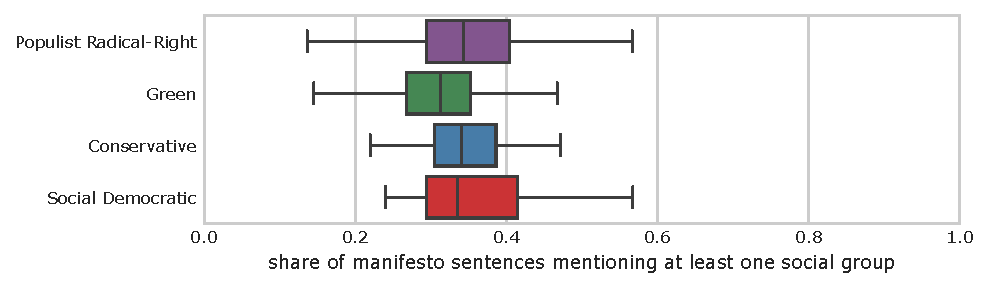
\includegraphics[keepaspectratio]{results/figures/figure01.pdf}
  \caption{\label{figure01}\protectShare of manifesto sentences mentioning at least one social group, by party family based on social group mentions extracted with our fine-tuned RoBERTa model. The boxplots show the distribution across manifestos within each party family, excluding outliers.}
\end{figure}%

Figure~\ref{figure01} summarizes the distributions of manifesto-level group mention prevalence estimates for the four party families covered by our corpus.
For each party manifesto, we compute the prevalence of social group mentions as the share of its sentences that contain at least one social group mention according to our classifier.
The box plots summarize the distribution of these manifesto-level estimates by party family.
This shows that typically between 30 and 40\% of sentences contain one social group mentions or more in the sample of manifestos we analyze.

\subsubsection{Attribute classification}\label{attribute-classification}

To classify the attributes contained in the social group mentions identified \revised{by our supervised mention detection classifier in the previous step, we applied our taxonomy to collect multi-label annotations for a sample of mentions.}

\paragraph{Annotation}\label{annotation}

Our coding instrument shows one mention at a time in its sentence context.\footnote{See Section~\ref{sec-coding_instrument} for details.}
Its coding logic reflects the structure of our taxonomy (cf.~Table \ref{table01}), which organizes attribute dimensions and categories across levels of abstraction and allows classifying a mention into multiple attribute categories if the group it refers to or describes is characterized by more than one kind of attribute.
Accordingly, we first ask the coder whether the group mention qualifies as a ``universal'' group reference, and, if not, prompt them to select all economic and non-economic attribute categories that are contained in the group mention.
A coder's classification of a mention as ``universal'' rules out classification of the mention's economic and non-economic attributes.
However, any non-universal mention could be labeled with one or more of the available attribute categories.

Two trained research assistants independently annotated the attributes contained in mentions in our sample.
Based on prior work (e.g., Thau 2019; Huber 2021; Dolinsky et al. 2025), we expected some attribute categories to be much less common.
We therefore used several annotation rounds to address label class imbalance and diversify the annotated sample.\footnote{Label class imbalance is common in social science classification and can harm predictive performance.
  Iterative sampling guided by prediction uncertainty can help mitigate this.}
We detail these steps in the Supporting Materials, Section~\ref{sec-apx_attribute_classification}, and summarize the main points here.
The first rounds focused on sampling diverse and difficult cases and balancing attribute prevalence.
Inter-annotator agreement was generally high, except in rounds where we strategically oversampled difficult cases or rare categories (see Table~\ref{tableC01} and Table~\ref{tableC02}).
To further improve annotation quality, the author team arbitrated disagreements, conducted a consolidation round, and reviewed cases where classifier ensembles disagreed with annotations.

In total, we collected, reviewed, and consolidated multi-label attribute annotations for 600 mention-in-context examples.
We demonstrate further below that few-shot learning enabled us to train reliable classifiers with these data.
This is a comparatively small sample for two reasons.
First, developing an adequate coding instrument and guidelines for our novel taxonomy required substantial upfront investment in testing and coder training.
Second, multi-label annotation is resource-intensive: annotating 600 examples amounts to an estimated 6,900 coding decisions per annotator, since each non-universal mention must be evaluated against all 14 attribute categories.\footnote{At an estimated prevalence of universal mentions at 25\%, 150 of 600 examples only require one coding decision (universal or not) whereas the other 450 examples required the universal-or-not decision \emph{plus} one binary decision (Yes/No) for each of our 14 attribute categories (\(=450 \times(1+4+10) = 6,750\)).}
However, we expect that the labeled data and fine-tuned classifiers we contribute will enable future work to scale the human annotation process we propose more efficiently.

The considerable human resource investments required to implement our multi-label classification scheme through manual annotation motivated us to pay particular attention to the quality of the annotations we collected.
In few-shot learning especially, few consistently labeled examples often yield better fine-tuning results than many noisily labeled examples.
The author team therefore arbitrated disagreements, conducted a consolidation round, and reviewed cases where classifier ensembles disagreed with annotations (see Section~\ref{sec-apx_attribute_classification}).

\paragraph{Automation}\label{automation}

\revised{The annotated mention-in-context examples} covered only a small fraction of the \revised{68,341 unique} predicted social group mentions.
We thus needed to automate attribute classification for all mentions.

Current computational text analysis methods offer two main approaches for multi-label classification with few annotated examples: few-shot fine-tuning with encoder-only models (Devlin et al. 2019) or few-shot in-context learning with decoder-only large language models (Brown et al. 2020).
We chose the first for its efficiency and proven effectiveness (cf. Tunstall et al. 2022), leaving the second for future work.

Specifically, we relied on the few-shot sentence transformer fine-tuning (SetFit) approach\footnote{Tunstall et al. (2022) show that the SetFit approach enables effective few-shot learning in text classification applications.
  SetFit is also more compute-efficient at prediction time compared to natural language inference (NLI) used by Horne et al. (2025) (Laurer et al. (2024)), which multiplies the number of inferences needed by the number of label categories.
  Relying on SetFit thus allows faster and more resource-saving automated coding of unlabeled social group mentions.} proposed by Tunstall et al. (2022) to train two separate multi-label classifiers -- one for economic attributes and one for non-economic attributes.
In the SetFit framework, labeled examples in the training set are first used to construct pairs for contrastive embedding model fine-tuning.
\revised{The contrastive embedding finetuning task practically augments our 600 annotated examples to several thousand contrastive pairs, providing ample training material for embedding model fine-tuning that effectively tunes the text representations that go into the next step: training an attribute category multi-label classification model.}
\revised{The classification head is the component that maps a mention's embedding into a multi-label attribute classification.}
\revised{Both components are trained end-to-end for multi-label classification on labeled examples.}

Having thoroughly evaluated several implementation choices, we found that inputting only the group mentions' text without the sentence context and using \href{https://huggingface.co/sentence-transformers/all-mpnet-base-v2}{\texttt{all-mpnet-base-v2}} as the base embedding model (Reimers and Gurevych 2019) performed best in our application.
Details about our implementation can be found in Section~\ref{sec-apx_setfit}.

\begin{table}[!th]
\centering
\caption{Evaluation results of group mention attribute classifiers. Values report the mean precision, recall, and F1-score averaged across five folds for each attribute category, along with the prevalence of each category in the training set.}
\label{table02}
\begin{tabular}{rrrrr}
\toprule
 & F1-Score & Precision & Recall & prevalence \\
\midrule
\textbf{economic attributes} &  &  &  &  \\
micro average & 0.785 & 0.822 & 0.758 &  \\
weighted average & 0.784 & 0.831 & 0.758 &  \\
macro average & 0.800 & 0.842 & 0.788 &  \\
\quad \textit{education} & 0.942 & 0.933 & 0.967 & 0.033 \\
\quad \textit{employment status} & 0.721 & 0.770 & 0.733 & 0.059 \\
\quad \textit{income/wealth/economic status} & 0.751 & 0.857 & 0.675 & 0.093 \\
\quad \textit{occupation/profession} & 0.787 & 0.809 & 0.776 & 0.166 \\
\cmidrule(lr){0-4}
\textbf{non-economic attributes} &  &  &  &  \\
micro average & 0.829 & 0.881 & 0.782 &  \\
weighted average & 0.826 & 0.896 & 0.782 &  \\
macro average & 0.804 & 0.871 & 0.768 &  \\
\quad \textit{age} & 0.872 & 0.918 & 0.841 & 0.106 \\
\quad \textit{crime} & 0.764 & 0.842 & 0.719 & 0.052 \\
\quad \textit{ethnicity} & 0.921 & 1.000 & 0.860 & 0.065 \\
\quad \textit{family} & 0.905 & 0.873 & 0.972 & 0.098 \\
\quad \textit{gender/sexuality} & 0.765 & 0.825 & 0.725 & 0.074 \\
\quad \textit{health} & 0.732 & 0.863 & 0.666 & 0.056 \\
\quad \textit{nationality} & 0.819 & 0.890 & 0.764 & 0.128 \\
\quad \textit{place/location} & 0.750 & 0.837 & 0.702 & 0.033 \\
\quad \textit{religion} & 0.759 & 0.770 & 0.776 & 0.050 \\
\quad \textit{shared values/mentalities} & 0.753 & 0.889 & 0.660 & 0.135 \\
\bottomrule
\end{tabular}
\end{table}%

Table~\ref{table02} summarizes the performance of the resulting attribute category classifiers averaged across five held-out test folds.\footnote{These are the results of models trained on folds' respective training examples using ``optimal'' hyper-parameters identified using hyperparameter grid search and early stopping based on macro-averaged F1 on the fold's validation examples.
}
The economic attribute classifier achieves a macro (micro) average F1 of 0.8 (0.785); the non-economic attribute classifier a macro (micro) average F1 of 0.804 (0.829).
We consider the performance of our classifiers to be strong given the low number of few-shot training examples, strong label class imbalance, and novelty of our taxonomy.
The classifiers prove similarly reliable as trained human annotators (see Table~\ref{tableC02}) in classifying economic attributes and even more reliable in classifying non-economic attributes.
And while classification reliability varies across attribute categories, it is overall very good, with most categories achieving an F1 of 0.75 or higher.
Moreover, the variation in classification reliability across attribute categories is not correlated with attribute categories' prevalence in the training data (see last column of Table~\ref{table02}), which suggests that performance differences are explained by task difficulty rather than mere lack of training material.
Nevertheless, we expect that future work will be able to improve on our results by collecting more (informative) training data, for example by leveraging our pre-trained classifiers or LLMs as (collaborative) annotators.
And measurement error introduced by our classifier in downstream regression analysis of specific attribute categories can be adjusted using error correction frameworks like design-based supervised learning (Egami et al. 2023).

\paragraph{{Validation}}\label{validation}

To assess the validity of our classifiers, we conduct three analyses reported in full in Section~\ref{sec-apx_validity}. First, a ``fighting words'' lexical analysis (Monroe et al. 2008) shows that the most distinctive terms for each attribute category align strongly with substantive expectations.
For instance, \emph{education} is characterized by terms like ``students'', ``pupils'', ``school'', and ``university'', while \emph{shared values/mentalities} features value-laden adjectives and lemmas of ``society''.
However, despite the distinctiveness of these terms, our analysis shows that simple keyword dictionaries cannot reliably replace our classifiers: the recall of the top-10 most distinctive terms is below 50\% for attribute categories such as \emph{religion} (42\%), \emph{nationality} (36\%), \emph{income/wealth/economic status} (33\%), and \emph{occupation/profession} (20\%).
These findings underscore the validity of supervised classification in our application.

Second, comparisons to group reference classifications in existing categorization schemes (Thau 2019; Horne et al. 2025) underscore the added value of our attribute-centered, multi-label, hierarchical taxonomy.
Comparing our attribute-centered group reference classifications to those in Thau (2019) reveals strong convergence where expected (e.g., 91\% of his \emph{Age/generation} mentions are classified as \emph{age} by our classifier, and 87\% of his \emph{Professional group} mentions as \emph{occupation/profession}), but also that his single-label scheme conceals meaningful attribute combinations: mentions in a given Thau category are frequently assigned to multiple attribute categories in our scheme.
Comparing our classifications to those obtained with the multi-label group category scheme of Horne et al. (2025), in turn, shows that both schemes partition the social group mentions in our corpus overall very similarly, as indicated by expected positive associations between occupation-related categories and systematic negative associations between non-economic and occupation/class-based categories.
However, our attribute-centered framework decomposes some of Horne et al.'s broad categories (e.g., \emph{Ethnic And National Communities}) into finer-grained attribute combinations while grouping very specific ones (e.g., their many specific occupational group categories) while also capturing group mentions not covered by any of their pre-defined categories.
Taken together, these analyses provide strong evidence of the content validity of our classifiers and clarify the analytical added value of our attribute-centered, multi-label measurement approach.

\section{\texorpdfstring{\revised{Prevalence of attribute dimensions, categories, and their combinations}}{Prevalence of attribute dimensions, categories, and their combinations}}\label{prevalence-of-attribute-dimensions-categories-and-their-combinations}

We now turn to descriptive statistics of the attribute classifications we have obtained for all social group mentions extracted by our group mention detection model in the sentences of manifestos in our corpus.
Note that we include in this analysis also group mentions in manifestos of centre-left and -right parties in the four countries covered by our case selection.

\begin{figure}[!th]
  \centering
  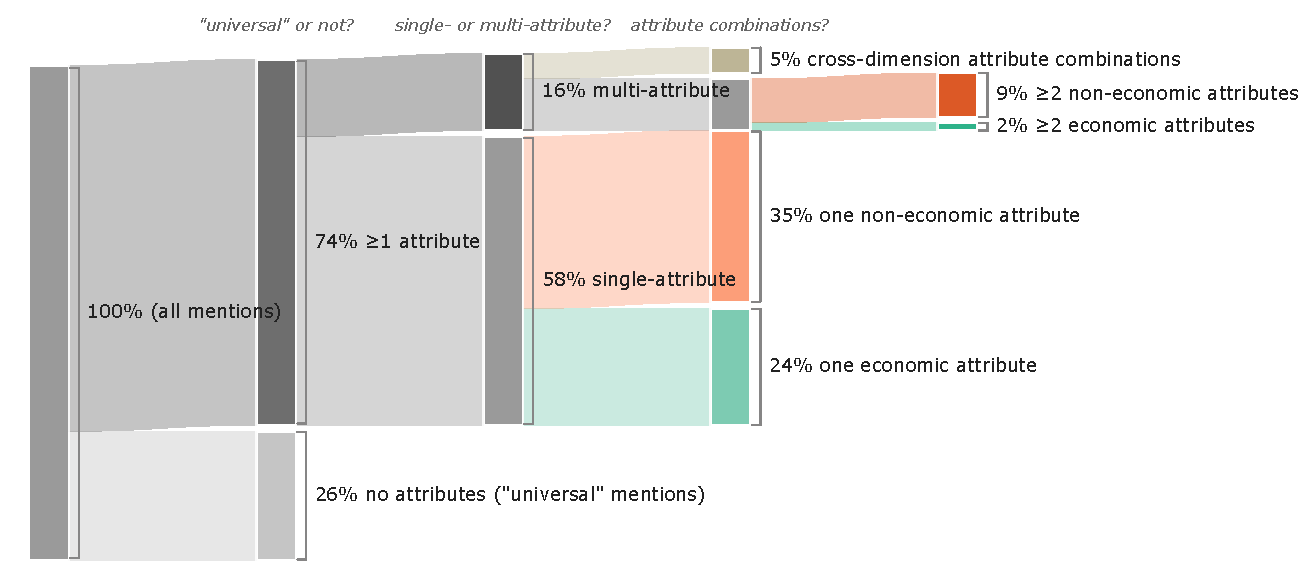
\includegraphics[keepaspectratio,width=\linewidth]{results/figures/figure02.pdf}
  \caption{\label{figure02}\protectSankey diagram showing the breakdown of social group mentions by attribute prevalence and attribute combinations. The leftmost column shows the total number of mentions extracted in our manifesto sentences corpus, which are then split into "universal" mentions (no predicted attributes) and mentions with at least one predicted attribute. The latter are further divided into single-attribute and multi-attribute mentions, with multi-attribute mentions split into those with only within-dimension combinations and those with cross-dimension combinations. The rightmost column shows the breakdown of within-dimension combinations into economic and non-economic attributes.}
\end{figure}%

First, Figure~\ref{figure02} presents a breakdown of the distribution of the number of attribute categories into which our classifiers assigned the social group mentions we have identified in our corpus.\footnote{We use a 0.5 threshold for predicted probabilities of attribute categories.}
This shows that the majority of social group mentions (74\%) we identify in the manifestos in our corpus feature at least one attribute covered by our taxonomy.
The rest are ``universal'' mentions according to our definition, meaning that they do not feature any economic or non-economic attributes in our taxonomy.

Among the 74\% non-universal social group mentions, slightly less than four out of five mentions (79\%) are predicted to feature only a single attribute (58\% of the total population).
About 60\% of these mentions feature a non-economic attribute and 40\% an economic attribute -- a first indication that non-economic attributes are more frequently invoked to refer to social groups than economic attributes.
However, 21\% of social group mentions we classify as non-universal (16\% of all mentions) are predicted to feature more than one social attribute.

We turn next to the overall prevalence of individual attribute categories among non-universal mentions.
The prevalence of an attribute category is the share of social group mentions predicted to feature that category.

\begin{figure}[!th]
  \centering
  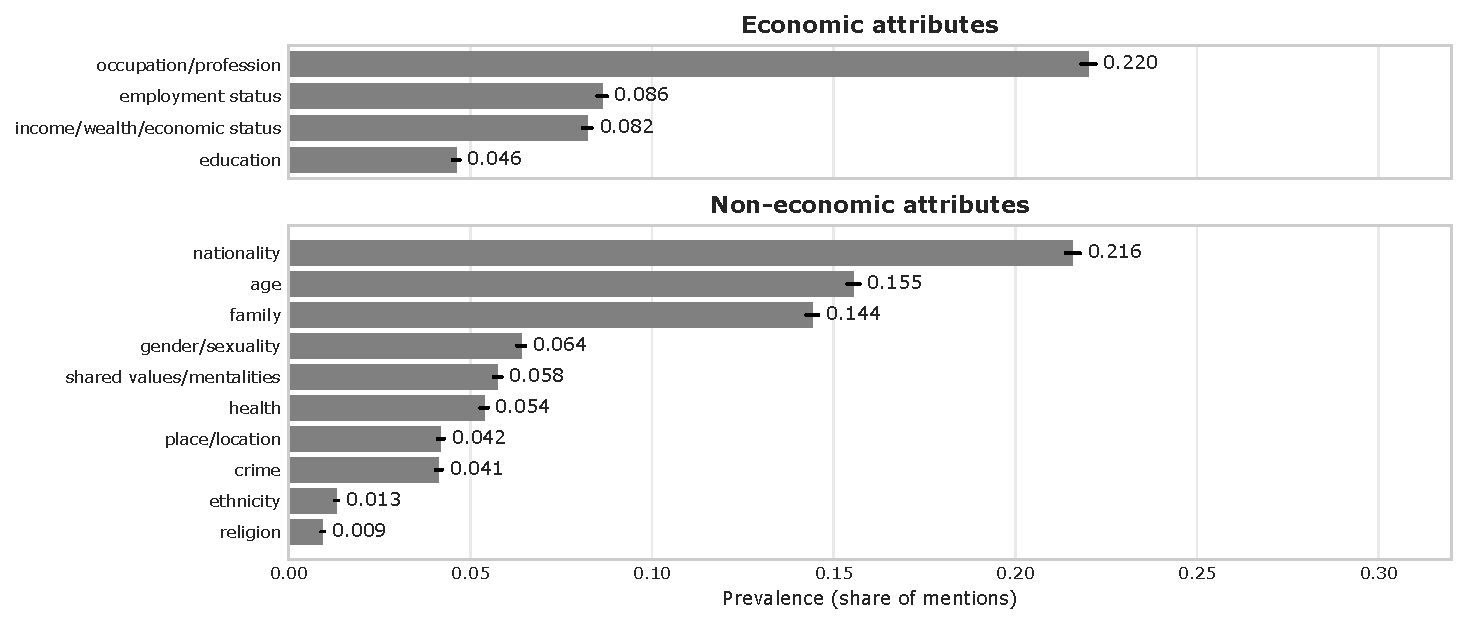
\includegraphics[keepaspectratio,width=\linewidth]{results/figures/figure03.pdf}
  \caption{\label{figure03}\protectPrevalence of attribute categories across all social group mentions (excluding universal mentions with no specific attributes). Bars show the share of mentions featuring each attribute, with 95\% confidence intervals. Top panel: economic attributes; bottom panel: non-economic attributes.}
\end{figure}%

Figure~\ref{figure03} shows that \emph{occupation/profession} is the most prevalent economic category and \emph{nationality} the most prevalent non-economic category.
The second and third most prevalent economic attributes (\emph{employment status} and \emph{income/wealth/economic status}) are relatively far less prevalent than the second and third most prevalent non-economic attributes (\emph{age} and \emph{family}), which show substantially higher prevalence.

Notably, the non-economic \emph{shared values/mentalities} category we introduce is predicted to occur in almost 6\% of non-universal social group mentions, and thus more often than the least prevalent economic attribute category (\emph{education}) as well as more often than five out of the remaining nine non-economic attribute categories.
This underscores the added value of introducing this novel category in our taxonomy.
We discuss attribute category prevalence again when focusing on differences across party families in Section~\ref{sec-structural_expectations}.

\begin{figure}[!th]
  \centering
  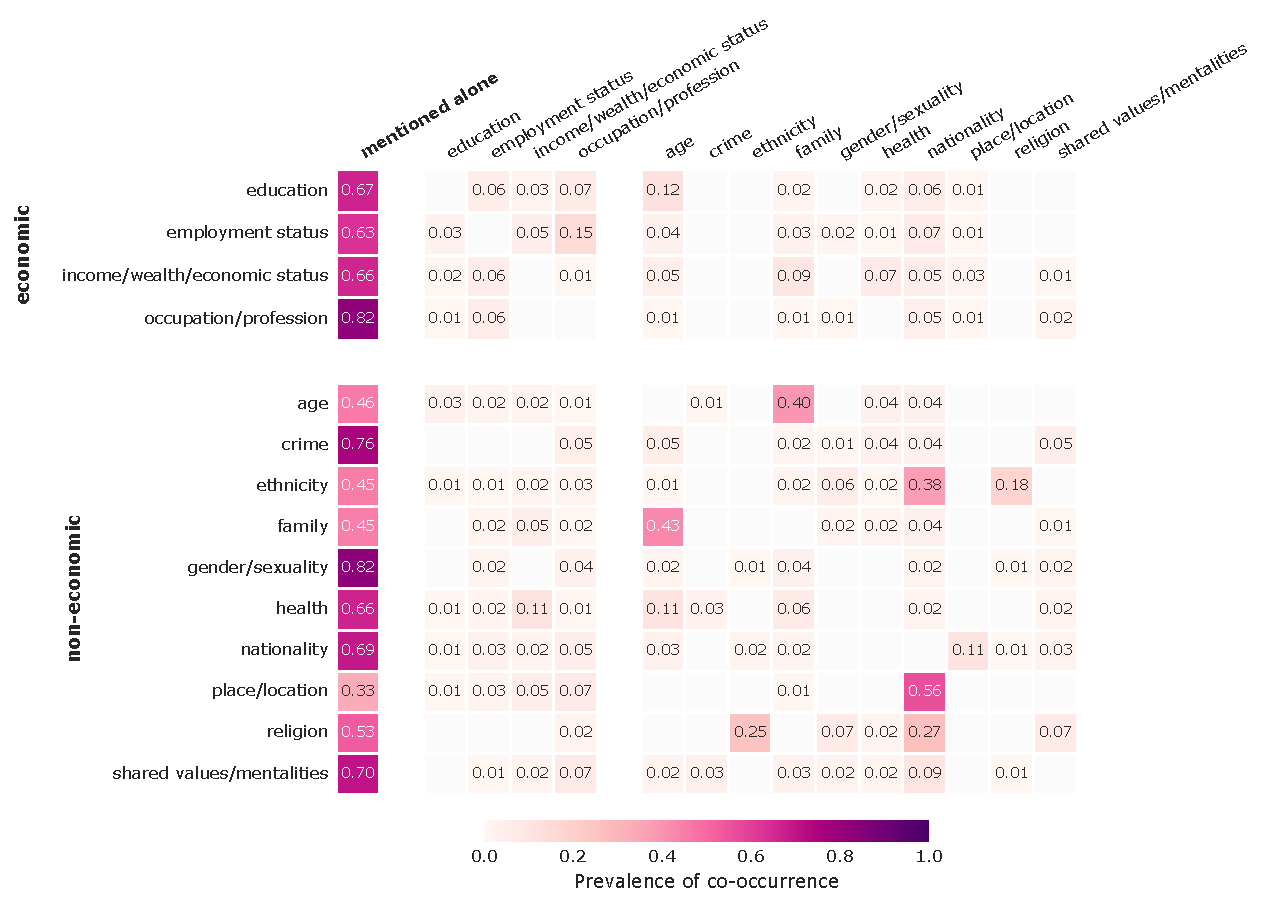
\includegraphics[keepaspectratio,width=\linewidth]{results/figures/figure04.pdf}
  \caption{\label{figure04}\protectCo-occurrence patterns of attribute categories in social group mentions. Heatmap cells show the share of mentions where each focal attribute (rows) co-occurs with other attributes (columns). The first column ('mentioned alone') shows the share of mentions where the focal attribute appears without any other attributes. Top panel: economic attributes; bottom panel: non-economic attributes. Values below 0.01 are not displayed.}
\end{figure}%

\unchanged{To gain a more granular understanding of attribute combination patterns at the group mention level in our data, we next compare attribute categories' co-occurrences.}
Recall that Figure~\ref{figure02} showed that if a party uses attributes to invoke social groups in their manifestos, it combines attributes from different categories about one out of five times.
Among such multi-attribute mentions, about two thirds feature ``within-dimension'' attribute combinations, that is, combinations of attributes from categories of the same attribute dimension (e.g., combinations of \emph{education} and \emph{employment status} as in ``students, who are working longer hours to fund their university study'').
Such within-dimension attribute combinations are about four times more frequent among non-economic attributes, which -- viewed together with the higher prevalence of non-economic attributes -- underscores the importance of non-economic attributes in parties' social group mentions.
In contrast, we estimate that every third multi-attribute social group mention combines economic with non-economic attributes (e.g., \emph{employment status} and \emph{health} as in ``persons with disabilities employed in a sheltered workshop'').

The first plot panel column in Figure~\ref{figure04} reports how likely each attribute category appears alone in a group mention.
This reveals substantial variation across mentions in different attribute categories in their tendencies to be single-attribute.
Among economic attributes, \emph{occupation/profession} is mentioned most frequently as the only kind of attribute in a social group mention (82\%).
This is about 1.3 times more often than the economic attribute that is most frequently combined with attributes from other categories: \emph{employment status}, which occurs alone in only 63\% of mentions that feature attributes of this category.
Among non-economic attributes, \emph{gender/sexuality} is mentioned most frequently alone (82\%) -- almost 2.5 times more often than \emph{place/location} (33\%).

Focusing on the two right-most heatmap columns in Figure~\ref{figure04}, which show attribute categories' co-occurrence tendencies, moreover allows examining specific combination patterns.\footnote{Figure~\ref{figureD04} reports an alternative visual presentation of co-occurrence patterns
  by analyzing co-occurrence patterns using \emph{conditional probabilities} of co-occurrence for all attribute category pairs.
  Table~\ref{tableD01} shows concrete examples sampled from our corpus.}
This view reveals that most of economic within-dimension attribute combination is driven by the combination of \emph{employment status} with other economic attributes.
For non-economic attributes, the stronger tendency of within-dimension attribute combination is driven by the frequent co-occurrence of \emph{age} and \emph{family}, and of \emph{ethnicity}, \emph{place/location}, or \emph{religion} with \emph{nationality}.

Regarding cross-dimension attribute combinations, economic attributes are frequently combined with \emph{age} (especially \emph{education}), \emph{family}, \emph{health}, and \emph{nationality}.
The non-economic attribute \emph{health} is often combined with \emph{income/wealth/economic status}.
And \emph{place/location} and \emph{shared values/mentalities} are often combined with \emph{occupation/profession}.

These patterns are particularly interesting because they add depth to the analysis of parties' group attribute focus.
For example, while social group mentions featuring descriptions of \emph{shared values/mentalities} are comparatively rare, their tendency to co-occur with \emph{occupation/profession} and \emph{nationality} suggests that parties use such attributes to differentiate their group focus strategies and specify which kind of people they mean exactly when referring to groups.

\section{Understanding social group references across analytical levels}\label{understanding-social-group-references-across-analytical-levels}

The taxonomy developed in this paper not only provides a framework for classifying social group references but also clarifies the analytical level at which different theories of party--group relations make their primary claims.
Rather than viewing these perspectives as competing explanations, we argue, in line with Westheuser and Zollinger (2025), that they primarily emphasize different -- yet partly overlapping -- layers in the political formation of social groups.
Distinguishing these layers allows their theoretical expectations to be evaluated separately while avoiding the incorporation of theoretical assumptions directly into the measurement of social groups.

Socio-structural approaches to party competition -- including cleavage theory, dealignment, and more recent accounts of partisan realignment -- are primarily concerned with which social groups become politically salient, expecting parties to mobilize groups that reflect enduring social structures and evolving electoral coalitions (Lipset and Rokkan 1967; Dalton 1984, 2008; Kriesi et al. 2008, 2012; Piketty 2018; Gethin et al. 2021).
Constructivist approaches, in turn, shift attention from the structural existence of social groups to the political processes through which they are constituted and acquire political meaning (Chandra 2012; de Leon 2014; Wolkenstein and Wratil 2021; Zuber et al. 2025).
Because these processes rely on symbolic interpretation, constructivist approaches naturally overlap with theories of political framing and identity formation (Westheuser 2025; Westheuser and Zollinger 2025; Zollinger 2022, 2024).

A related body of work focuses primarily on how already constituted social groups are politically interpreted and evaluated. Research on deservingness and the social construction of target populations examines whether groups are portrayed as deserving or undeserving, threatening or vulnerable, productive or dependent, or as members of a shared political community (Entman 1993; Schneider and Ingram 1993; van Oorschot 2000, 2006). These approaches generally treat the referenced groups as analytically given, focusing on their evaluation rather than on the processes through which they are defined (Theiss 2023; Deiss-Helbig et al. 2026; Esmark and Schoop 2017). Political framing, however, is broader than this final evaluative layer. Parties can frame social conflict by selecting which group-defining attributes to invoke, by combining attributes into particular group constructions, and by attaching evaluative meanings to the resulting groups (cf. Entman (1993)). Our analytical distinction therefore does not imply that framing occurs only at the final stage; rather, we distinguish the evaluation of already constituted groups from the prior selection and combination of attributes through which groups are defined.

By separating group-defining attributes from subsequent framing, our taxonomy provides a common measurement framework within which these perspectives can be examined individually or in combination.
In the following, we illustrate this analytical distinction by deriving expectations from each perspective and comparing them to the patterns observed in party manifestos.

\subsubsection{Socio-structural expectations}\label{sec-structural_expectations}

Socio-structural theories imply that differences in party competition should primarily become visible in the selection of social attributes.
Because parties mobilize electoral coalitions rooted in different social positions and conflict structures, they are expected to differ systematically in the types of groups they invoke (Lipset and Rokkan 1967; Kriesi et al. 2008, 2012; Bornschier 2015; Piketty 2018; Gethin et al. 2021).
The attribute-centered nature of our taxonomy allows these expectations to be examined across multiple levels of abstraction, from broad attribute dimensions to increasingly specific group references.

For example, Green parties are expected to place greater emphasis on social groups associated with the winners of post-industrial transformation, including highly educated professionals, younger cohorts, women, and groups linked to emerging socio-cultural conflicts (Marks et al. 2018; Bornschier 2015; Westheuser and Zollinger 2025).
Populist radical right (PRR) parties, by contrast, should emphasize nationally bounded groups, manual and technical occupations, and groups associated with the economic and cultural consequences of globalization, educational expansion, and immigration (Mudde 2007; Kriesi et al. 2008; Stubager 2009).

These expectations should become increasingly pronounced across the hierarchy of our taxonomy.
At the level of attribute dimensions, both Green and PRR parties should rely more strongly on non-economic attributes than their centre-left and centre-right competitors, reflecting the growing importance of socio-cultural conflicts in contemporary party competition.
At the level of attribute categories, however, clearer differences should emerge.
Green parties are expected to place greater emphasis on gender and sexuality, age, and socio-cultural occupations, whereas PRR parties should focus more strongly on nationality and occupations associated with production, security, and traditional labour markets.
Finally, at the level of specific group references, these differences should translate into distinct repertoires of groups, such as women, LGBTQI+ persons, students, and socio-cultural professionals for Green parties, compared with manual workers, farmers, police, entrepreneurs, or nationally defined communities for PRR parties.

\afterpage{
  \clearpage
  \thispagestyle{empty}
  \begin{figure}[p]
    \centering
    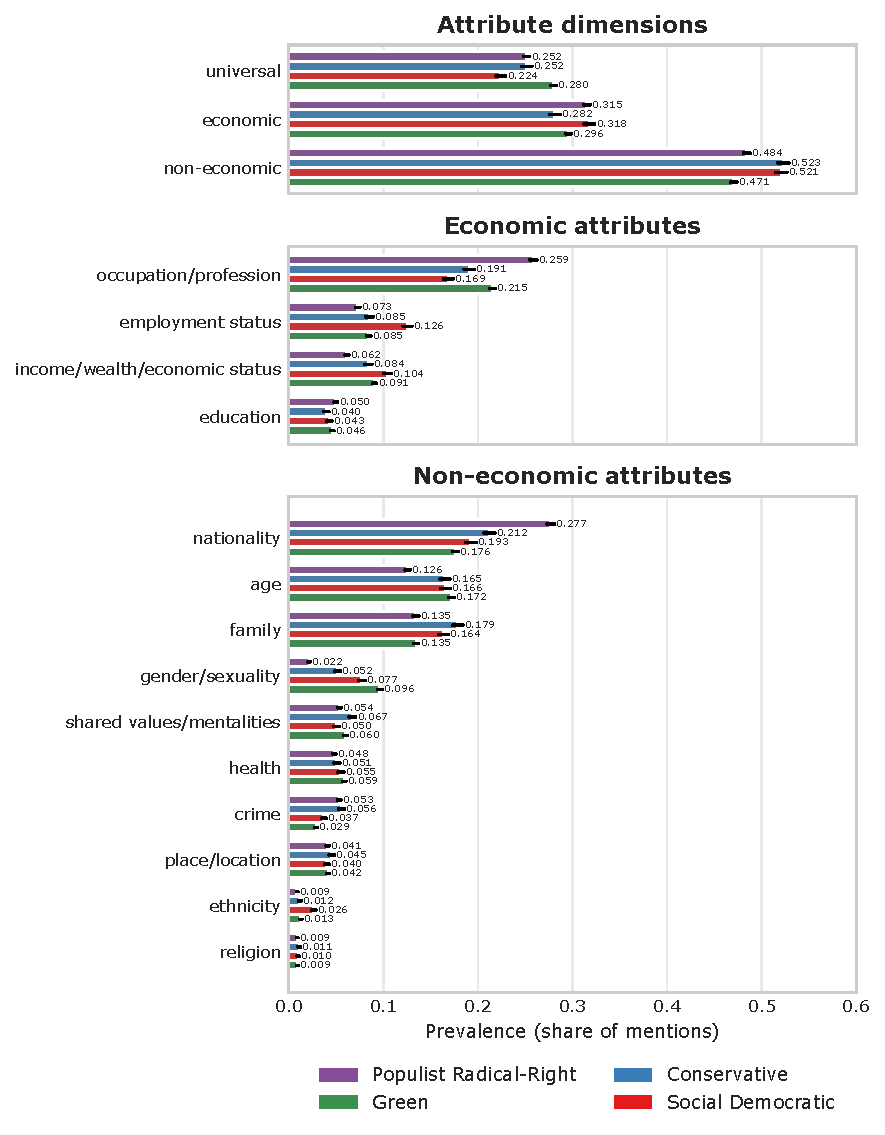
\includegraphics[keepaspectratio,width=\linewidth]{results/figures/figure05.pdf}
    \caption{\label{figure05}\protectPrevalence of attribute dimensions in all mentions and economic and non-economic attributes in non-universal social group mentions in parties' election manifestos by party family. Bars show share of mentions containing each attribute, with 95\% confidence intervals. \emph{Note:} Top panel shows prevalence in all mentions, while middle and bottom panels show prevalence in mentions containing at least one attribute.}
  \end{figure}%
  \clearpage
}

Figure~\ref{figure05} compares the prevalence of attribute dimensions and categories across Green, PRR, centre-left, and centre-right parties.
Contrary to a common interpretation of contemporary party competition, the four party families differ little in the overall balance between economic and non-economic group references.
Across all party families, non-economic attributes occur roughly one and a half to two times more frequently than economic attributes, while references lacking either type of attribute (universal references) occur at comparable rates.
Thus, the prominence of non-economic group references is not distinctive to Green and PRR parties but characterizes centre-left and -right parties as well.

Differences emerge, however, once attention shifts from broad attribute dimensions to specific attribute categories. Within the economic dimension, both Green and PRR parties rely more heavily on occupational attributes than their mainstream competitors, although this tendency is considerably stronger among PRR parties.
By contrast, PRR parties place comparatively little emphasis on employment status and income-related attributes, distinguishing them particularly from social democratic parties.
Within the non-economic dimension, Green parties attach substantially greater importance to gender- and age-related attributes, whereas PRR parties are distinguished by their strong emphasis on nationality.
Interestingly, references to family-related groups are most common among centre-left and -right parties rather than among the challenger parties.

These patterns remain remarkably stable over time (see Figure~\ref{figureD01} and Figure~\ref{figureD02}) and closely resemble those observed in a sample covering a wider range of Conservative and Social Democratic parties (see Figure~\ref{figureD03}), suggesting that they are not an artefact of the party sample used for the main analysis.

Moving to the most specific level of the taxonomy further illustrates how party families differentiate through the concrete groups they invoke.
To examine how parties populate a given attribute category with different social groups, we employ fighting words analysis (Monroe et al. 2008), which identifies the terms that are statistically most characteristic of one party family relative to another within a given subset of group references.
The fighting words analyses in Figure~\ref{figure06} show that Green parties' gender- and sexuality-related group references are characterized by terms relating to homosexuality, non-binary gender identities, and intersections with health and migration.
PRR parties, by contrast, associate gender primarily with fertility, birth, childrearing, and traditional family roles.
Similar differences emerge for occupational references.
PRR parties most distinctively invoke members of the armed forces, entrepreneurs, bureaucrats, and the judiciary (cf. Dolinsky et al. 2025), whereas Green parties emphasize socio-cultural and educational professionals, intellectuals, and lifestyle-related groups.

\begin{figure}[!th]
  \begin{minipage}{\linewidth}
    \centering
    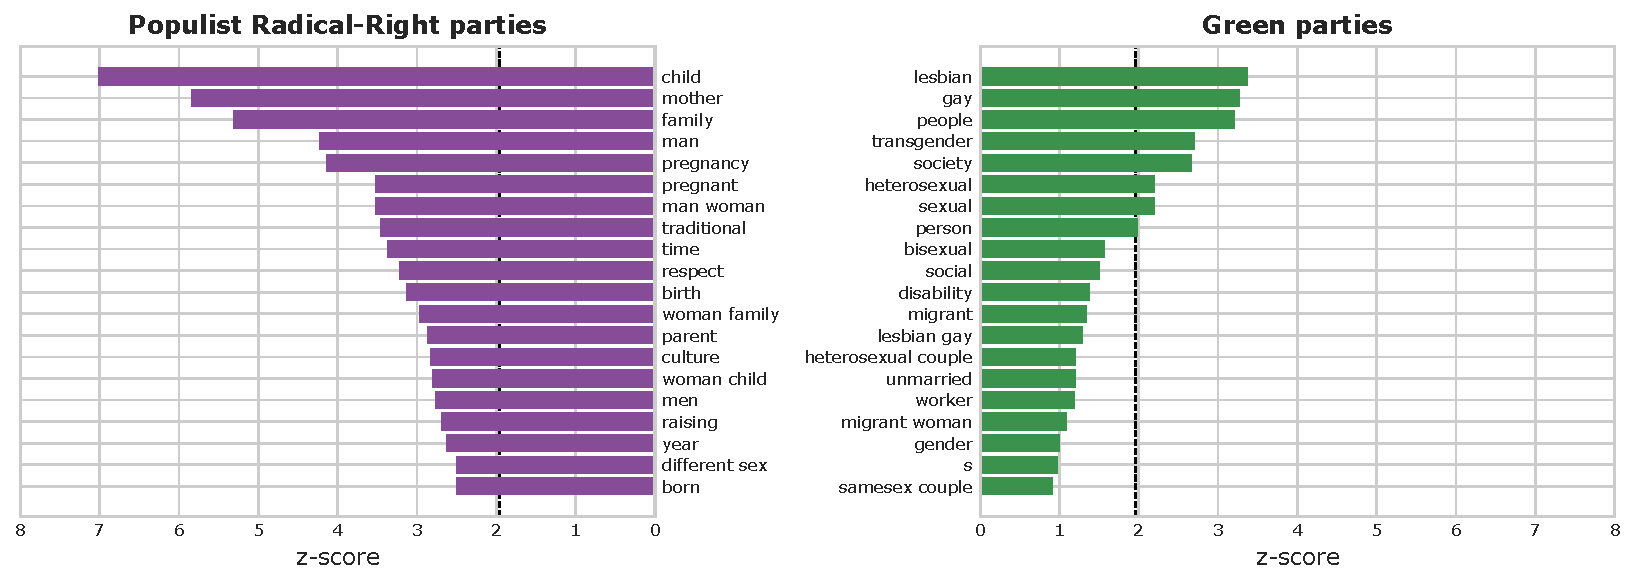
\includegraphics[keepaspectratio,width=\linewidth]{results/figures/figure06a.pdf}
    \subcaption{\label{figure06a}\protectGender/sexuality-related social group mentions}
  \end{minipage}%
  \newline
  \begin{minipage}{\linewidth}
    \centering
    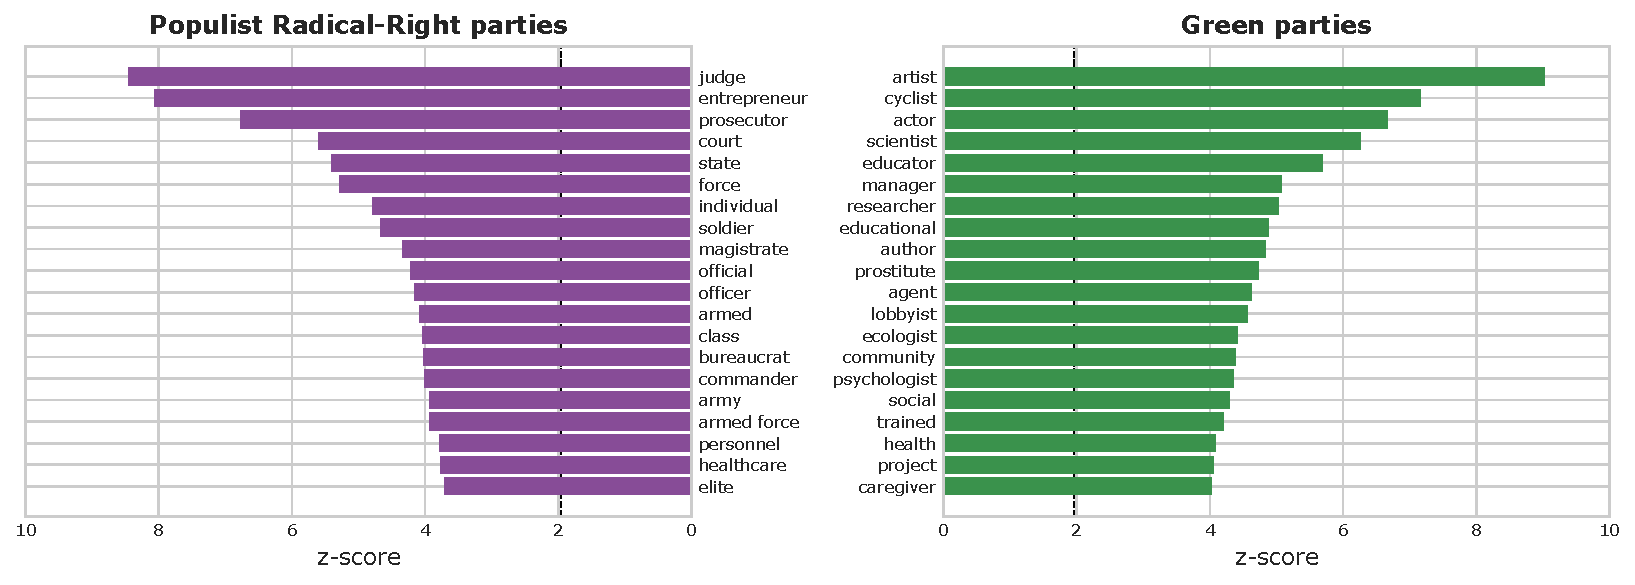
\includegraphics[keepaspectratio,width=\linewidth]{results/figures/figure06b.pdf}
    \subcaption{\label{figure06b}\protectOccupation/profession-related social group mentions}
  \end{minipage}%
  \caption{\label{figure06}\protectMost distinctive words of group mentions in selected attribute categories in Populist Radical-Right and Green parties' election manifestos. Values plotted are $z$-scores from ``fighting words'' analysis. Values above ±1.96 (vertical dashed line) can be considered significantly distinctive.}
\end{figure}%

\subsubsection{Constructivist expectations}\label{constructivist-expectations}

Constructivist approaches imply that differences between parties become particularly visible not in the prevalence of broad attribute categories but in the ways attributes are combined to construct politically meaningful social groups.
Rather than treating social groups as fixed expressions of underlying social structures, this literature emphasizes that political actors actively constitute groups by selecting, combining, and symbolically interpreting social attributes (Chandra 2012; Brubaker 2004; de Leon 2014; Wolkenstein and Wratil 2021; Zuber et al. 2025).

A central mechanism in this process is moral boundary-making.
Political actors distinguish us from them not only through socio-demographic attributes but also through shared values, lifestyles, and moral dispositions (Lamont 1992, 2009; Wimmer 2013; Westheuser 2025; Westheuser and Zollinger 2025).
Importantly, morality can play two analytically distinct roles.
Moral attributes may themselves define a social group -- for example, the ``hard-working'' or ``ordinary'' people -- or they may combine with existing attributes to create narrower groups, such as hard-working immigrants.
By contrast, moral \emph{evaluations} as in ``immigrants are dangerous'' or ``welfare recipients are lazy'' do not redefine group membership but attach evaluative meaning to already constituted groups.
Following the analytical distinction developed in this paper, we therefore treat the former as instances of group construction, whereas the latter belong to the subsequent layer of political framing.

These considerations imply two expectations.
First, constructivist approaches should become visible in attribute compositions, particularly where moral or value-related attributes combine with socio-demographic attributes to define new groups.
Second, they should become visible in groups constituted primarily through shared values, mentalities, or moral dispositions, because these attributes define collectivities independently of conventional socio-demographic characteristics.

Figure~\ref{figure07} examines attribute compositions in Green and PRR manifestos.
Several clear differences emerge.
PRR parties frequently combine nationality with occupational, family, crime, and especially shared-value attributes, thereby constructing nationally bounded social groups differentiated by moral characteristics.
Green parties, by contrast, more often combine age, gender, and economic attributes within individual group references.

Particularly striking is the role of shared values and mentalities.
Although both party families invoke value-based attributes with similar overall frequency (see Figure~\ref{figure05}), PRR parties combine these attributes much more frequently with other defining characteristics, especially nationality and occupation.
Rather than merely mobilizing existing socio-demographic groups, they therefore construct politically meaningful groups through combinations of structural and moral attributes.

\begin{figure}[!th]
  \centering
  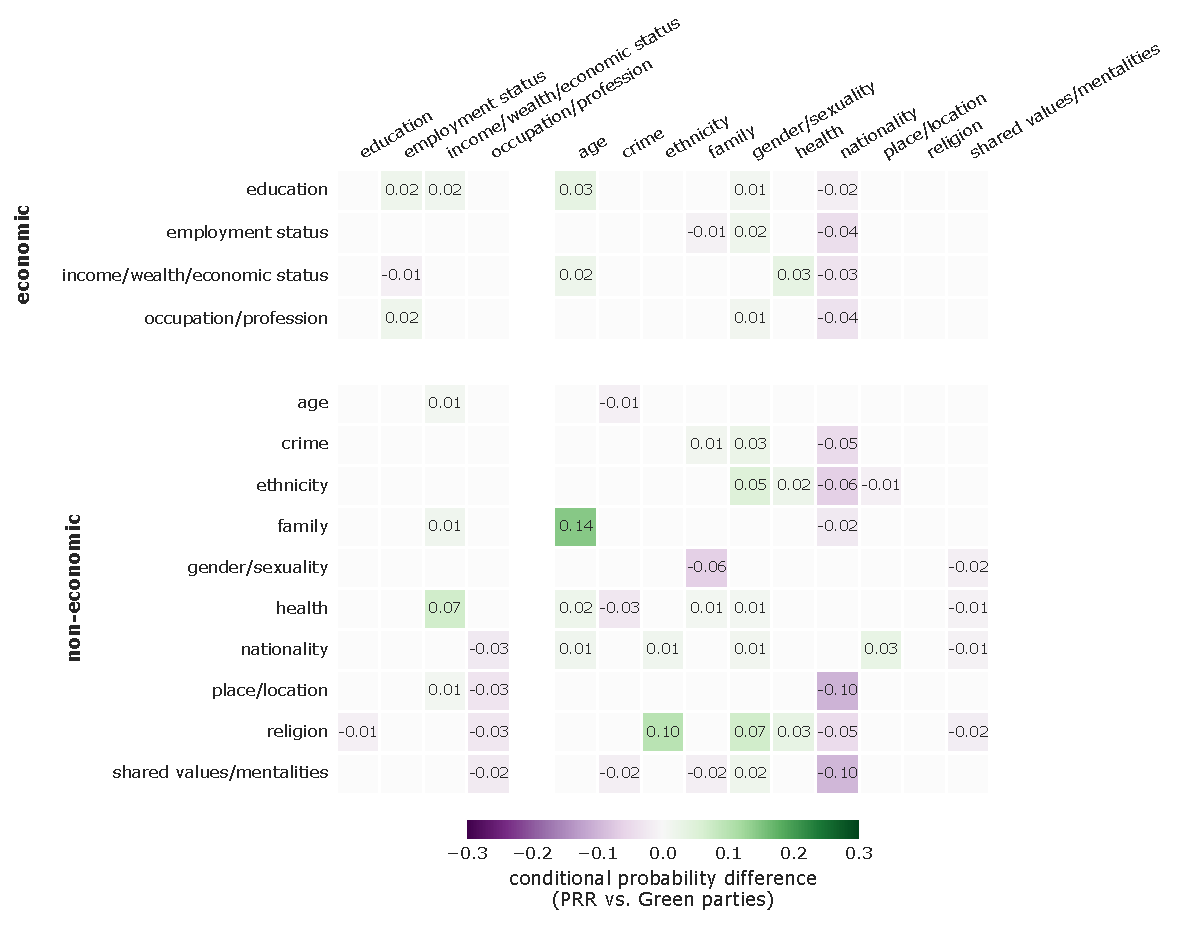
\includegraphics[keepaspectratio,width=\linewidth]{results/figures/figure07.pdf}
  \caption{\label{figure07}\protectDifferences in conditional probabilities of attribute co-occurrence between Green and Populist Radical-Right (PRR) party manifestos. Heatmap cells show the difference in $\Pr(B|A)$ between Green and PRR parties (Green – PRR). Rows indicate ``attribute A'' (the conditioning attribute) and columns indicate ``attribute B'' (the outcome attribute). Positive values (green) indicate that attribute B is more likely to be mentioned given attribute A in Green party manifestos compared to PRR manifestos, while negative values (purple) indicate the opposite. \emph{Note:} Values below 0.01 in absolute value are not displayed.}
\end{figure}%

Constructivist scholarship has argued that the universalist pole of contemporary political conflict is often articulated less explicitly than its particularist counterpart (Westheuser and Zollinger 2025).
Combining our taxonomy with a fighting words analysis allows us to examine this question directly.
Specifically, we focus on group references of Green and PRR parties in our corpus classified as involving shared values or mentalities that also invoke society.\footnote{In particular, we focus on the group mentions in this subset that contain the lemmas of the terms ``society'' and ``societies''.}
This allows us to contrast the constitutive value attributes through which Green and PRR parties define this otherwise universal collectivity.
Figure~\ref{figure08} shows that the two party families rely on markedly different repertoires of constitutive value attributes. Green parties predominantly define society through relational principles such as solidarity, sustainability, inclusion, justice, and openness, whereas PRR parties emphasize prosperity, freedom, health, activity, and national belonging.
Although references defined by shared values account for only around five to seven percent of all group mentions, they occupy a particularly important position within constructivist theories because they reveal the competing moral grammars through which parties define society itself.

\begin{figure}[!th]
  \centering
  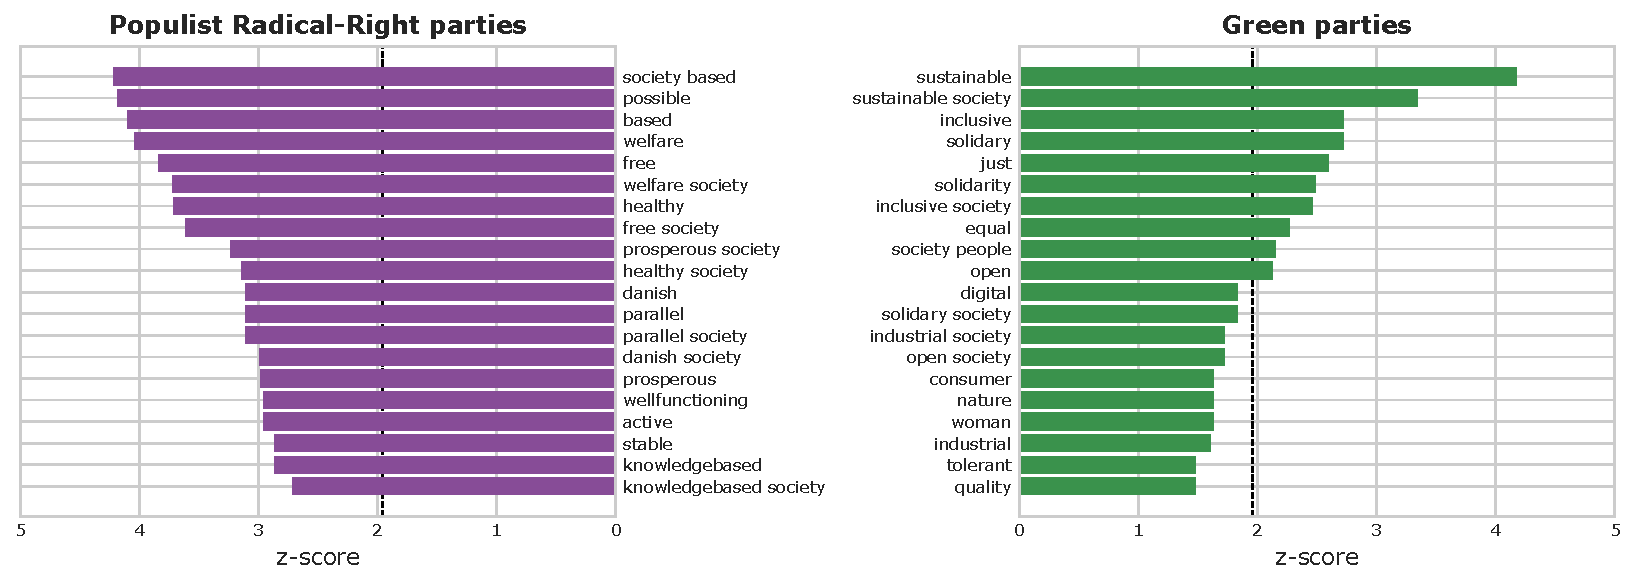
\includegraphics[keepaspectratio,width=\linewidth]{results/figures/figure08.pdf}
  \caption{\label{figure08}\protectMost distinctive words for mentions of \emph{shared values/mentalities}-based references to `society' in Populist Radical-Right and Green parties' election manifestos.  Values plotted are $z$-scores from ``fighting words'' analysis. Values above ±1.96 (vertical dashed line) can be considered significantly distinctive.}
\end{figure}%

\subsubsection{Group evaluation and deservingness}\label{group-evaluation-and-deservingness}

Approaches to deservingness and group evaluation shift attention from the definition and construction of social groups to how already identified groups are portrayed in political communication. Whether migrants are described as contributors or free riders, workers as deserving producers or disadvantaged victims, entrepreneurs as innovators or privileged elites, or LGBTQI+ people as valued members of society or objects of political contestation cannot be inferred from group-defining attributes alone (Entman 1993; Schneider and Ingram 1993; van Oorschot 2000, 2006; Esmark and Schoop 2017).

Our taxonomy establishes the necessary analytical foundation for such analyses by systematically identifying the types of attributes emphasized in the referenced social groups. Evaluating parties' references to groups requires an additional analytical layer that captures the political stance or evaluative frame attached to each reference.



To illustrate this complementarity, we combine our attribute classifications with the stance classifier developed by Horne et al. (2025) \footnote{\href{https://huggingface.co/rwillh11/mdeberta_NLI_stance_NoContext}{\texttt{rwillh11/mdeberta\_NLI\_stance\_NoContext}} (accessed on July 8, 2026).} and examine how Green and PRR parties evaluate group references featuring gender and sexuality attributes.
Figure~\ref{figure09} first compares overall party stances towards these group references and subsequently distinguishes between the specific groups identified by Horne et al.'s taxonomy (men, women, and LGBTQI+ people).

\begin{figure}[!th]
  \centering
  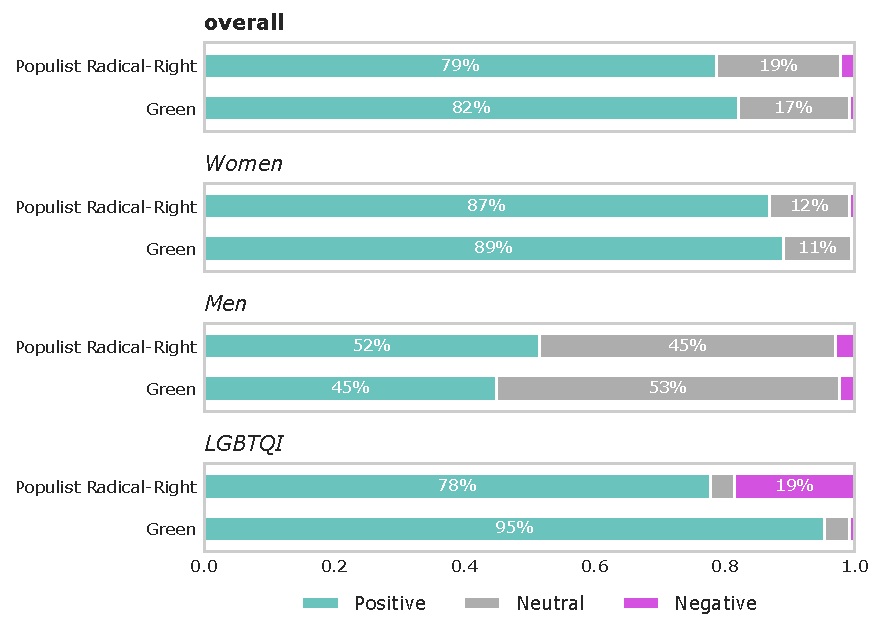
\includegraphics[keepaspectratio,width=\linewidth]{results/figures/figure09.pdf}
  \caption{\label{figure09}\protectStance distribution towards \emph{gender/sexuality}-related groups by party family. Top panel shows overall distribution across all gender/sexuality groups. Subsequent panels show distributions for specific group categories (LGBTQI, Men, Women), with bars comparing stance distributions between Populist Radical-Right and Green parties.}
\end{figure}%

At the aggregate level, Green and PRR parties differ surprisingly little.
References to gender- and sexuality-related groups are overwhelmingly positive in both party families, while explicitly negative references remain extremely rare.
This finding echoes a broader pattern in the literature on party group appeals, which has repeatedly shown that parties typically invoke social groups in supportive or representative terms rather than to criticize them (e.g., Thau 2019; Huber 2021; Riethmüller and Franzmann 2025; Horne et al. 2025).
This underscores that the prevalence of group references is an important dimension of group-based party competition -- much like issue salience in studies of issue competition.

However, once attention shifts to specific groups, pronounced differences emerge.
PRR parties express substantially more positive evaluations of men than Green parties, whereas Green parties overwhelmingly portray LGBTQI+ people positively.
By contrast, roughly one in five PRR references to LGBTQI+ people is negative.

Together, these findings illustrate why our taxonomy's separation of group identification from political evaluation is analytically productive: it allows socio-structural, constructivist, and deservingness perspectives to be examined within a common measurement framework.

\section{Conclusion}\label{conclusion}

This paper introduces an attribute-centered taxonomy for analyzing political parties' references to social groups together with a scalable measurement framework for identifying these references in political text.
By taking attributes rather than predefined social groups as the fundamental unit of classification, the taxonomy provides a common analytical language for studying how parties define social groups while remaining agnostic with respect to competing theories of party competition, representation, and group formation.

Beyond providing a new measurement framework, the taxonomy also clarifies the analytical layers at which different theories of party--group relations make their primary claims.
Socio-structural approaches primarily explain which social attributes become politically salient.
Constructivist approaches explain how parties combine and reinterpret these attributes to constitute politically meaningful groups.
Approaches to deservingness and group evaluation focus on how these groups are subsequently portrayed and evaluated.
Framing can occur across all three layers: through the selective invocation of attributes, their combination into particular group constructions, and the evaluative meanings attached to the resulting groups.

Our empirical application illustrates the analytical value of this distinction.
Across more than five decades of party manifestos in 36 democracies, the taxonomy reveals that broad attribute dimensions conceal differences that become increasingly pronounced at more specific levels of abstraction.
While Green, populist radical right, centre-left, and centre-right parties rely on remarkably similar overall proportions of economic and non-economic group references, they differ systematically in the specific attributes they prioritize and, even more strongly, in how they combine these attributes to construct politically meaningful groups.
In particular, the analysis of attribute combinations and shared values demonstrates how parties actively organize familiar social attributes into competing conceptions of society that would remain difficult to detect using conventional group classifications.

Finally, the taxonomy establishes a common foundation for analyses that extend beyond the identification of social groups themselves.
Combining attribute classifications with stance or framing analysis makes it possible to distinguish who parties talk about, how they constitute these groups, and how they evaluate them.
More generally, the taxonomy provides a common organizational backbone for extending analyses to lower levels of abstraction.
Deductively, occupational references can be linked to ISCO, educational references to ISCED, or multiple attribute categories combined into broader schemes such as Oesch's class typology.
Inductively, approaches such as fighting words, topic modelling, or embedding-based clustering can uncover variation within attribute categories and identify emerging forms of group construction.

More broadly, our framework also speaks to a longstanding question in the study of party competition.
Both classical cleavage research and recent entrepreneurial accounts increasingly converge on the importance of social groups and political identities for understanding enduring ties between parties and citizens.
Yet, despite this renewed attention to political identities, their formation remains difficult to observe empirically.
As Westheuser and Zollinger (2025) put it, identity formation often resembles ``ships passing in the night'' (Westheuser and Zollinger 2025, 120).
Political identities are unlikely to be directly observable in isolated text units.
Instead, they emerge through the cumulative repetition of communicative practices: the recurring invocation of particular social groups, their constitution through combinations of attributes and symbolic boundaries, and their repeated evaluation through political framing.
By separating these communicative building blocks, our taxonomy provides a common measurement framework for studying how repeated patterns of group construction and political evaluation crystallize into enduring party--group identities -- and equally importantly, when they fail to do so.

% TODO: add for journal submission
\medskip
\input{funding.tex}
\input{coi.tex}

\section{References}\label{references}

\begingroup
%\setlength{\bibsep}{2pt}
\setstretch{1.15}

\phantomsection\label{refs}
\begin{CSLReferences}{1}{0}
\bibitem[\citeproctext]{ref-amarales_group_2025}
Amarales, A. R., L. Bellodi, and Catherine E. De Vries. 2025. {``\href{https://lucabellodi.com/material/group_appeals_mobilization_US.pdf}{Group Appeals and Political Mobilization: Evidence from {US} House Races}.''}

\bibitem[\citeproctext]{ref-bartolini_identity_2007}
Bartolini, Stefano, and Peter Mair. 2007. \emph{Identity, Competition and Electoral Availability: The Stabilisation of European Electorates 1885-1985}. ECPR Press.

\bibitem[\citeproctext]{ref-benoit_challenges_2009}
Benoit, Kenneth, Thomas Bräuninger, and Marc Debus. 2009. {``\href{https://doi.org/10.1080/09644000903055856}{Challenges for Estimating Policy Preferences: Announcing an Open Access Archive of Political Documents}.''} \emph{German Politics} 18 (3): 441--54.

\bibitem[\citeproctext]{ref-bornschier_cleavage_2010}
Bornschier, Simon. 2010. \emph{Cleavage Politics and the Populist Right: The New Cultural Conflict in Western Europe}. Temple University Press.

\bibitem[\citeproctext]{ref-bornschier_new_2015}
---------. 2015. {``The New Cultural Conflict, Polarization, and Representation in the Swiss Party System, 1975--2011.''} \emph{Swiss Political Science Review} 21 (4): 680--701.

\bibitem[\citeproctext]{ref-bornschier_cleavage_2024}
Bornschier, Simon, Lukas Haffert, Silja Häusermann, Marco Steenbergen, and Delia Zollinger. 2024. \emph{Cleavage Formation in the 21st Century: How Social Identities Shape Voting Behavior in Contexts of Electoral Realignment}. Cambridge University Press.

\bibitem[\citeproctext]{ref-brown_language_2020}
Brown, Tom B., Benjamin Mann, Nick Ryder, Melanie Subbiah, Jared Kaplan, Prafulla Dhariwal, Arvind Neelakantan, et al. 2020. {``\href{https://doi.org/10.48550/arXiv.2005.14165}{Language Models Are Few-Shot Learners}.''} {arXiv}.

\bibitem[\citeproctext]{ref-brubaker_ethnicity_2004}
Brubaker, Rogers. 2004. \emph{Ethnicity Without Groups}. Harvard University Press.

\bibitem[\citeproctext]{ref-chandra_constructivist_2012}
Chandra, Kanchan. 2012. \emph{Constructivist Theories of Ethnic Politics}. Oxford University Press.

\bibitem[\citeproctext]{ref-cramer_politics_2016}
Cramer, Katherine J. 2016. \emph{The Politics of Resentment: Rural Consciousness in Wisconsin and the Rise of Scott Walker}. University of Chicago Press.

\bibitem[\citeproctext]{ref-crenshaw_demarginalizing_1989}
Crenshaw, Kimberle. 1989. {``Demarginalizing the Intersection of Race and Sex.''} \emph{University of Chicago Legal Forum} 1989 (1): 139--67.

\bibitem[\citeproctext]{ref-dalton_cognitive_1984}
Dalton, Russell J. 1984. {``\href{https://doi.org/10.2307/2130444}{Cognitive Mobilization and Partisan Dealignment in Advanced Industrial Democracies}.''} \emph{The Journal of Politics} 46 (1): 264--84.

\bibitem[\citeproctext]{ref-dalton_citizen_2008}
---------. 2008. \emph{Citizen Politics: Public Opinion and Political Parties in Advanced Industrial Democracies}. 5th ed. {CQ} Press.

\bibitem[\citeproctext]{ref-damhuis_roads_2020}
Damhuis, Koen. 2020. \emph{Roads to the Radical Right: Understanding Different Forms of Electoral Support for Radical Right-Wing Parties in France and the Netherlands}. Oxford University Press.

\bibitem[\citeproctext]{ref-damhuis_responsive_2017}
Damhuis, Koen, and Johannes Karremans. 2017. {``\href{https://doi.org/10.1080/01402382.2017.1300472}{Responsive to Whom? A Comparison of the Mitterrand and Hollande Presidencies}.''} \emph{West European Politics} 40 (6): 1267--87.

\bibitem[\citeproctext]{ref-dausgaard_elite_2024}
Dausgaard, Christoffer H., and Frederik Hjorth. 2024. {``\href{https://fghjorth.github.io/workingpapers/runningtally.pdf}{Elite Rhetoric and the Running Tally of Party-Group Linkages}.''} Working paper. Working paper.

\bibitem[\citeproctext]{ref-de_mulder_who_2025}
De Mulder, August, Ine Gevers, and Željko Poljak. 2025. {``\href{https://doi.org/10.1177/00323217251325548}{Who Deserves Representation, and When? Unpacking the Temporal Dynamics of Politicians' Claims of Representation on Social Media}.''} \emph{Political Studies}, March, 00323217251325548.

\bibitem[\citeproctext]{ref-deiss-helbig_who_2026}
Deiss-Helbig, Elisa, Isabelle Guinaudeau, and Theres Matthieß. 2026. {``Who Deserves? Ideological Gaps in Citizens' Deservingness Perceptions.''} \emph{European Political Science Review}, 1--22.

\bibitem[\citeproctext]{ref-devlin_bert_2019}
Devlin, Jacob, Ming-Wei Chang, Kenton Lee, and Kristina Toutanova. 2019. {``\href{https://doi.org/10.48550/arXiv.1810.04805}{{BERT}: Pre-Training of Deep Bidirectional Transformers for Language Understanding}.''} {arXiv}.

\bibitem[\citeproctext]{ref-dobson_green_2012}
Dobson, Andrew. 2012. \emph{\href{https://doi.org/10.4324/9780203131671}{Green Political Thought}}. 0th ed. Routledge.

\bibitem[\citeproctext]{ref-dolinsky_parties_2023}
Dolinsky, Alona O., and Lena M. Huber. 2023. {``\href{https://doi.org/10.31219/osf.io/a9sf6_v1}{Parties' Group Appeals as Representative Claims: A New Perspective on Parties' Efforts to Connect with Voters}.''} {OSF}.

\bibitem[\citeproctext]{ref-dolinsky_manifestovault_2024}
Dolinsky, Alona O., Lena Maria Huber, and Will Horne. 2024. {``\href{https://doi.org/10.34894/VKQSPO}{{ManifestoVault V1.0: Annotated full-text general election manifestos at the natural-sentence level of three European countries 1970-2025}}.''} DataverseNL.

\bibitem[\citeproctext]{ref-dolinsky_who_2025}
Dolinsky, Alona O., Lena M. Huber, and Will Horne. 2025. {``\href{https://doi.org/10.31219/osf.io/64jwa_v1}{Who Do Parties Speak to? Introducing the {PSoGA}: A New Comprehensive Database of Parties' Social Group Appeals}.''} {OSF}.

\bibitem[\citeproctext]{ref-downs_economic_1957}
Downs, Anthony. 1957. \emph{An Economic Theory of Democracy}. Harper.

\bibitem[\citeproctext]{ref-egami_dsl_2023}
Egami, Naoki, Musashi Hinck, Brandon M. Stewart, and Hanying Wei. 2023. {``Using Imperfect Surrogates for Downstream Inference: Design-Based Supervised Learning for Social Science Applications of Large Language Models.''} In \emph{Proceedings of the 37th International Conference on Neural Information Processing Systems}. NIPS '23. Red Hook, NY, USA: Curran Associates Inc.

\bibitem[\citeproctext]{ref-eley_forging_2002}
Eley, Geoff. 2002. \emph{Forging Democracy: The History of the Left in Europe, 1850--2000}. Oxford University Press.

\bibitem[\citeproctext]{ref-entman_framing_1993}
Entman, Robert M. 1993. {``\href{https://doi.org/10.1111/j.1460-2466.1993.tb01304.x}{Framing: Toward Clarification of a Fractured Paradigm}.''} \emph{Journal of Communication} 43 (4): 51--58.

\bibitem[\citeproctext]{ref-esmark_deserving_2017}
Esmark, Anders, and Sarah R Schoop. 2017. {``Deserving Social Benefits? Political Framing and Media Framing of {`Deservingness'} in Two Welfare Reforms in Denmark.''} \emph{Journal of European Social Policy} 27 (5): 417--32.

\bibitem[\citeproctext]{ref-evans_new_2017}
Evans, Geoffrey, and James Tilley. 2017. \emph{The New Politics of Class: The Political Exclusion of the British Working Class}. Oxford University Press.

\bibitem[\citeproctext]{ref-fan_beyond_2020}
Fan, Angela, Shruti Bhosale, Holger Schwenk, Zhiyi Ma, Ahmed El-Kishky, Siddharth Goyal, Mandeep Baines, et al. 2020. {``\href{https://doi.org/10.48550/arXiv.2010.11125}{Beyond English-Centric Multilingual Machine Translation}.''} {arXiv}.

\bibitem[\citeproctext]{ref-ford_changing_2020}
Ford, Robert, and Will Jennings. 2020. {``The Changing Cleavage Politics of Western Europe.''} \emph{Annual Review of Political Science} 23 (1): 295--314.

\bibitem[\citeproctext]{ref-fraser_fortunes_2013}
Fraser, Nancy. 2013. \emph{Fortunes of Feminism: From State-Managed Capitalism to Neoliberal Crisis}. Brooklyn, {NY}: Verso Books.

\bibitem[\citeproctext]{ref-gethin_political_2021}
Gethin, Amory, Clara Martínez-Toledano, and Thomas Piketty. 2021. \emph{Political Cleavages and Social Inequalities: A Study of Fifty Democracies, 1948-2020}. Cambridge, Massachusetts: Harvard University Press.

\bibitem[\citeproctext]{ref-hooghe_cleavage_2018}
Hooghe, Liesbet, and Gary Marks. 2018. {``Cleavage Theory Meets Europe's Crises: Lipset, Rokkan, and the Transnational Cleavage.''} \emph{Journal of European Public Policy} 25 (1): 109--35.

\bibitem[\citeproctext]{ref-horn_political_2021}
Horn, Alexander, Anthony Kevins, Carsten Jensen, and Kees Van Kersbergen. 2021. {``\href{https://doi.org/10.1177/1354068820907998}{Political Parties and Social Groups: New Perspectives and Data on Group and Policy Appeals}.''} \emph{Party Politics} 27 (5): 983--95.

\bibitem[\citeproctext]{ref-horne_using_2025}
Horne, Will, Alona O. Dolinsky, and Lena M. Huber. 2025. {``\href{https://doi.org/10.31219/osf.io/fp2h3_v2}{Using {LLMs} to Detect Group Appeals in Parties' Election Manifestos}.''} {OSF}.

\bibitem[\citeproctext]{ref-howe_nationalism_2022}
Howe, Philip J., Edina Szöcsik, and Christina I. Zuber. 2022. {``\href{https://doi.org/10.1177/00104140211036033}{Nationalism, Class, and Status: How Nationalists Use Policy Offers and Group Appeals to Attract a New Electorate}.''} \emph{Comparative Political Studies} 55 (5): 832--68.

\bibitem[\citeproctext]{ref-huber_beyond_2021}
Huber, Lena Maria. 2021. {``\href{https://doi.org/10.1080/10584609.2021.1998264}{Beyond Policy: The Use of Social Group Appeals in Party Communication}.''} \emph{Political Communication} 39 (3): 293--310.

\bibitem[\citeproctext]{ref-huber_social_2024}
Huber, Lena Maria, Thomas M. Meyer, and Markus Wagner. 2024. {``\href{https://doi.org/10.1086/729946}{Social Group Appeals in Party Rhetoric: Effects on Policy Support and Polarization}.''} \emph{The Journal of Politics} 86 (4): 1304--18.

\bibitem[\citeproctext]{ref-ivanusch_manifesto_2024}
Ivanusch, Christoph, and Sven Regel. 2024. {``Manifesto Corpus Translation.''} Berlin: Wissenschaftszentrum Berlin f{ü}r Sozialforschung (WZB)/G{ö}ttingen~\ldots.

\bibitem[\citeproctext]{ref-kaufman_selecting_2024}
Kaufman, Aaron R. 2024. {``\href{https://www.cambridge.org/core/journals/political-analysis/article/selecting-more-informative-training-sets-with-fewer-observations/FCC76C9F7A5B27D00B0C9BE023BF84E7}{Selecting More Informative Training Sets with Fewer Observations}.''} \emph{Political Analysis} 32 (1): 133--39.

\bibitem[\citeproctext]{ref-kriesi_political_2012}
Kriesi, Hanspeter, Edgar Grande, Martin Dolezal, Marc Helbling, Dominic Höglinger, Swen Hutter, and Bruno W\{\textbackslash textbackslash\}üest. 2012. \emph{Political Conflict in Western Europe}. Cambridge University Press.

\bibitem[\citeproctext]{ref-kriesi_west_2008}
Kriesi, Hanspeter, Edgar Grande, Romain Lachat, Martin Dolezal, Simon Bornschier, and Timotheos Frey. 2008. \emph{West European Politics in the Age of Globalization}. Cambridge University Press.

\bibitem[\citeproctext]{ref-laclau_populist_2005}
Laclau, Ernesto. 2005. \emph{On Populist Reason}. Verso.

\bibitem[\citeproctext]{ref-lamont_money_1992}
Lamont, Michèle. 1992. \emph{Money, Morals, and Manners: The Culture of the French and the American Upper-Middle Class}. University of Chicago Press.

\bibitem[\citeproctext]{ref-lamont_dignity_2000}
---------. 2009. \emph{The Dignity of Working Men: Morality and the Boundaries of Race, Class, and Immigration}. Harvard University Press.

\bibitem[\citeproctext]{ref-lamont_study_2002}
Lamont, Michèle, and Virág Molnár. 2002. {``\href{https://doi.org/10.1146/annurev.soc.28.110601.141107}{The Study of Boundaries in the Social Sciences}.''} \emph{Annual Review of Sociology} 28 (1): 167--95.

\bibitem[\citeproctext]{ref-laurer_less_2024}
Laurer, Moritz, Wouter van Atteveldt, Andreu Casas, and Kasper Welbers. 2024. {``\href{https://doi.org/10.1017/pan.2023.20}{Less Annotating, More Classifying: Addressing the Data Scarcity Issue of Supervised Machine Learning with Deep Transfer Learning and {BERT}-{NLI}}.''} \emph{Political Analysis} 32 (1): 84--100.

\bibitem[\citeproctext]{ref-lehmann_manifesto_2023}
Lehmann, Pola, Simon Franzmann, Tobias Burst, Theres Matthieß, Sven Regel, Felicia Riethmüller, Andrea Volkens, et al. 2023. {``\href{https://doi.org/10.25522/MANIFESTO.MPDS.2023A}{Manifesto Project Dataset}.''} Manifesto Project.

\bibitem[\citeproctext]{ref-de_leon_party_2014}
de Leon, Cedric. 2014. \emph{Party \& Society: Reconstructing a Sociology of Democratic Party Politics}. Political Sociology Series. Cambridge, {UK} Malden, {MA}: Polity.

\bibitem[\citeproctext]{ref-licht_measuring_2025}
Licht, Hauke, Tarik Abou-Chadi, Pablo Barberá, and Whitney Hua. 2025. {``\href{https://doi.org/10.1086/730711}{Measuring and Understanding Parties' Anti-Elite Strategies}.''} \emph{The Journal of Politics}, January.

\bibitem[\citeproctext]{ref-licht_going_2023}
Licht, Hauke, and Fabienne Lind. 2023. {``\href{https://doi.org/10.5117/CCR2023.2.2.LICH}{Going Cross-Lingual: A Guide to Multilingual Text Analysis}.''} \emph{Computational Communication Research} 5 (2).

\bibitem[\citeproctext]{ref-licht_detecting_2025}
Licht, Hauke, and Ronja Sczepanski. 2025. {``\href{https://doi.org/10.1017/S0007123424000954}{Detecting Group Mentions in Political Rhetoric: A Supervised Learning Approach}.''} \emph{British Journal of Political Science} 55 (January): e119.

\bibitem[\citeproctext]{ref-licht_validating_2026}
Licht, Hauke, Ronja Sczepanski, Moritz Laurer, and Ayjeren Bekmuratovna. 2026. {``\href{https://doi.org/10.31219/osf.io/9trjs}{Validating Open-Source Machine Translation for Quantitative Text Analysis}.''} {OSF} Preprints.

\bibitem[\citeproctext]{ref-lipset_cleavage_1967}
Lipset, Seymour Martin, and Stein Rokkan. 1967. {``Cleavage Structures, Party Systems, and Voter Alignments.''} Edited by Seymour Martin Lipset and Stein Rokkan. \emph{Party Systems and Voter Alignments}, 1--64.

\bibitem[\citeproctext]{ref-hooghe_marks_2018}
Marks, Gary, David Attewell, Jan Rovny, and Liesbet Hooghe. 2018. {``The Social Bases of the Transnational Cleavage.''} \emph{Unpublished Manuscript}.

\bibitem[\citeproctext]{ref-mccall_complexity_2005}
McCall, Leslie. 2005. {``\href{https://doi.org/10.1086/426800}{The Complexity of Intersectionality}.''} \emph{Signs} 30 (3): 1771--1800.

\bibitem[\citeproctext]{ref-miller_active_2020}
Miller, Blake, Fridolin Linder, and Walter R. Mebane. 2020. {``\href{https://doi.org/10.1017/pan.2020.4}{Active Learning Approaches for Labeling Text: Review and Assessment of the Performance of Active Learning Approaches}.''} \emph{Political Analysis} 28 (4): 532--51.

\bibitem[\citeproctext]{ref-monroe_fightin_2008}
Monroe, Burt L., Michael P. Colaresi, and Kevin M. Quinn. 2008. {``\href{https://doi.org/10.1093/pan/mpn018}{Fightin' Words: Lexical Feature Selection and Evaluation for Identifying the Content of Political Conflict}.''} \emph{Political Analysis} 16 (4): 372--403.

\bibitem[\citeproctext]{ref-mudde_populist_2007}
Mudde, Cas. 2007. \emph{Populist Radical Right Parties in Europe}. Cambridge University Press.

\bibitem[\citeproctext]{ref-mudde_populism_2017}
Mudde, Cas, and Cristobal Rovira Kaltwasser. 2017. \emph{Populism: A Very Short Introduction}. Oxford University Press.

\bibitem[\citeproctext]{ref-oesch_redrawing_2006}
Oesch, Daniel. 2006. \emph{Redrawing the Class Map: Stratification and Institutions in Britain, Germany, Sweden and Switzerland}. Springer.

\bibitem[\citeproctext]{ref-van_oorschot_who_2000}
Oorschot, Wim van. 2000. {``Who Should Get What, and Why? On Deservingness Criteria and the Conditionality of Solidarity Among the Public.''} \emph{Policy \& Politics} 28 (1): 33--48.

\bibitem[\citeproctext]{ref-van_oorschot_making_2006}
---------. 2006. {``Making the Difference in Social Europe: Deservingness Perceptions Among Citizens of European Welfare States.''} \emph{Journal of European Social Policy} 16 (1): 23--42.

\bibitem[\citeproctext]{ref-piketty_brahmin_2018}
Piketty, Thomas. 2018. {``\href{https://ideas.repec.org//p/hal/psewpa/hal-02878211.html}{Brahmin Left Vs Merchant Right: Rising Inequality \& the Changing Structure of Political Conflict}.''} \emph{{PSE} Working Papers}.

\bibitem[\citeproctext]{ref-pitkin_concept_1967}
Pitkin, Hanna Fenichel. 1967. \emph{The Concept of Representation}. University of California Press.

\bibitem[\citeproctext]{ref-polanyi_great_1944}
Polanyi, Karl. 1944. \emph{The Great Transformation: The Political and Economic Origins of Our Time}. Boston: Beacon Press.

\bibitem[\citeproctext]{ref-przeworski_paper_1986}
Przeworski, Adam, and John Sprague. 1986. \emph{Paper Stones: A History of Electoral Socialism}. University of Chicago Press.

\bibitem[\citeproctext]{ref-reimers_sentence-bert_2019}
Reimers, Nils, and Iryna Gurevych. 2019. {``\href{https://doi.org/10.48550/arXiv.1908.10084}{Sentence-{BERT}: Sentence Embeddings Using Siamese {BERT}-Networks}.''} {arXiv}.

\bibitem[\citeproctext]{ref-riethmuller_supply-side_2025}
Riethmüller, Felicia, and Simon T Franzmann. 2025. {``\href{https://doi.org/10.1177/13540688251339624}{Supply-Side Dynamics of Parties' Group Appeals: How Dominance Affects the Choice Between Symbolic and Policy-Based Appeals}.''} \emph{Party Politics}, May, 13540688251339624.

\bibitem[\citeproctext]{ref-riker_theory_1962}
Riker, William H. 1962. \emph{The Theory of Political Coalitions}. Yale University Press.

\bibitem[\citeproctext]{ref-roth_greens_2021}
Röth, Leonce, and Hanna Schwander. 2021. {``\href{https://doi.org/10.1080/01402382.2019.1702792}{Greens in Government: The Distributive Policies of a Culturally Progressive Force}.''} \emph{West European Politics} 44 (3): 661--89.

\bibitem[\citeproctext]{ref-schneider_social_1993}
Schneider, Anne, and Helen Ingram. 1993. {``\href{https://doi.org/10.2307/2939044}{Social Construction of Target Populations: Implications for Politics and Policy}.''} \emph{The American Political Science Review} 87 (2): 334--47.

\bibitem[\citeproctext]{ref-sczepanski_who_2023}
Sczepanski, Ronja. 2023. {``\href{https://doi.org/10.1177/00104140231194054}{Who Are the Cosmopolitans? How Perceived Social Sorting and Social Identities Relate to European and National Identities}.''} \emph{Comparative Political Studies}, August, 00104140231194054.

\bibitem[\citeproctext]{ref-stewart_crisis_2000}
Stewart, Frances. 2000. {``Crisis Prevention: Tackling Horizontal Inequalities.''} \emph{Oxford Development Studies} 28 (3): 245--62.

\bibitem[\citeproctext]{ref-stewart_horizontal_2016}
---------. 2016. \emph{Horizontal Inequalities and Conflict: Understanding Group Violence in Multiethnic Societies}. Springer.

\bibitem[\citeproctext]{ref-stubager_2009}
Stubager, Rune. 2009. {``Education-Based Group Identity and Consciousness in the Authoritarian-Libertarian Value Conflict.''} \emph{European Journal of Political Research} 48 (2): 204--33.

\bibitem[\citeproctext]{ref-stuckelberger_group_2024}
Stuckelberger, Simon, and Anke Tresch. 2024. {``\href{https://doi.org/10.1177/00323217221123147}{Group Appeals of Parties in Times of Economic and Identity Conflicts and Realignment}.''} \emph{Political Studies} 72 (2): 463--85.

\bibitem[\citeproctext]{ref-taylor_identity_2023}
Taylor, Sean J., Lev Muchnik, Madhav Kumar, and Sinan Aral. 2023. {``\href{https://doi.org/10.1038/s41562-022-01459-8}{Identity Effects in Social Media}.''} \emph{Nature Human Behaviour} 7 (1): 27--37.

\bibitem[\citeproctext]{ref-thau_how_2019}
Thau, Mads. 2019. {``\href{https://doi.org/10.1177/0032321717744495}{How Political Parties Use Group-Based Appeals: Evidence from Britain 1964--2015}.''} \emph{Political Studies} 67 (1): 63--82.

\bibitem[\citeproctext]{ref-thau_social_2021}
---------. 2021. {``\href{https://doi.org/10.1086/710018}{The Social Divisions of Politics: How Parties' Group-Based Appeals Influence Social Group Differences in Vote Choice}.''} \emph{The Journal of Politics} 83 (2): 675--88.

\bibitem[\citeproctext]{ref-theiss_how_2023}
Theiss, Maria. 2023. {``How Does the Content of Deservingness Criteria Differ for More and Less Deserving Target Groups? An Analysis of Polish Online Debates on Refugees and Families with Children.''} \emph{Journal of Social Policy} 52 (4): 962--80.

\bibitem[\citeproctext]{ref-tunstall_efficient_2022}
Tunstall, Lewis, Nils Reimers, Unso Eun Seo Jo, Luke Bates, Daniel Korat, Moshe Wasserblat, and Oren Pereg. 2022. {``\href{https://doi.org/10.48550/arXiv.2209.11055}{Efficient Few-Shot Learning Without Prompts}.''} {arXiv}.

\bibitem[\citeproctext]{ref-westheuser_moral_2025}
Westheuser, Linus. 2025. {``Boundaries and Cleavages: Elements of a Cultural Sociology of Political Divides.''} \emph{European Journal of Cultural and Political Sociology} 12 (3): 289--313.

\bibitem[\citeproctext]{ref-westheuser_cleavage_2025}
Westheuser, Linus, and Delia Zollinger. 2025. {``\href{https://doi.org/10.1017/S1755773924000249}{Cleavage Theory Meets Bourdieu: Studying the Role of Group Identities in Cleavage Formation}.''} \emph{European Political Science Review} 17 (1): 110--27.

\bibitem[\citeproctext]{ref-lamont_missing_2014}
Wimmer, Andreas. 2013. \emph{Ethnic Boundary Making: Institutions, Power, Networks}. Oxford University Press.

\bibitem[\citeproctext]{ref-wolkenstein_multidimensional_2021}
Wolkenstein, Fabio, and Christopher Wratil. 2021. {``\href{https://doi.org/10.1111/ajps.12563}{Multidimensional Representation}.''} \emph{American Journal of Political Science} 65 (4): 862--76.

\bibitem[\citeproctext]{ref-zollinger_cleavage_2022}
Zollinger, Delia. 2022. {``\href{https://doi.org/10.1111/ajps.12743}{Cleavage Identities in Voters' Own Words: Harnessing Open-Ended Survey Responses}.''} \emph{American Journal of Political Science} 0 (0).

\bibitem[\citeproctext]{ref-zollinger_place-based_2024}
---------. 2024. {``Place-Based Identities and Cleavage Formation in the Knowledge Society.''} \emph{Electoral Studies} 88: 102768.

\bibitem[\citeproctext]{ref-zuber_group_2025}
Zuber, Christina I., Philip J. Howe, and Edina Szöcsik. 2025. {``Group Identities and Party Competition.''} Working Paper. Working Paper.

\end{CSLReferences}

\endgroup

\clearpage
\appendix
\setcounter{page}{1}
\begin{center}
\Huge \scshape Supplemental Materials \par
\LARGE \bfseries Attributes, Abstractions, and Combinations \par
\end{center}
\vfill
\renewcommand{\contentsname}{Contents}
\startcontents[appendix]
\printcontents[appendix]{}{1}{\setcounter{tocdepth}{2}}
\vfill
\clearpage

\counterwithin{figure}{section}
\counterwithin{table}{section}
\renewcommand\thefigure{\thesection\arabic{figure}}
\renewcommand\thetable{\thesection\arabic{table}}

\section{Dataset}\label{sec-apx_dataset}

We focus our application on social group references in the party manifestos of populist radical-right (PRR) and Green parties.
To this end, we compiled a corpus of party manifestos from 36 Western countries covering the period 1966--2021.
To enable comparisons with mainstream parties, we additionally include the manifestos of centre-left/social democratic and centre-right/conservative parties in four selected countries: Germany, Sweden, United Kingdom, and the United States.
Figure~\ref{figureA03} provides an overview of all covered cases.

Manifesto texts were obtained from secondary data sources, \emph{Manifesto Project Dataset} (Lehmann et al. 2023) and PoliDoc (Benoit et al. 2009).
Remaining gaps were filled through original data collection where possible.

In order to classify parties as being PRRPs, we follow the definition of Mudde (2007) and see nationalism as their core ideological feature.
For Green parties we follow Röth and Schwander (2021) or Dobson (2012) who define Green parties by a strong emphasis of ecologism and environmentalism and typically, but not always, incorporate the term ``Green'' in their party names.

In total, we processed 494 party manifestos (202 Green, 182 PRR, 56 Social Democratic, and 54 Conservative) into a corpus comprising 436,941 sentences.
Figure~\ref{figureA01} and Figure~\ref{figureA02} shows an overview of the number of manifestos and sentences by party family included in our corpus.

\begin{figure}[!th]
  \centering
  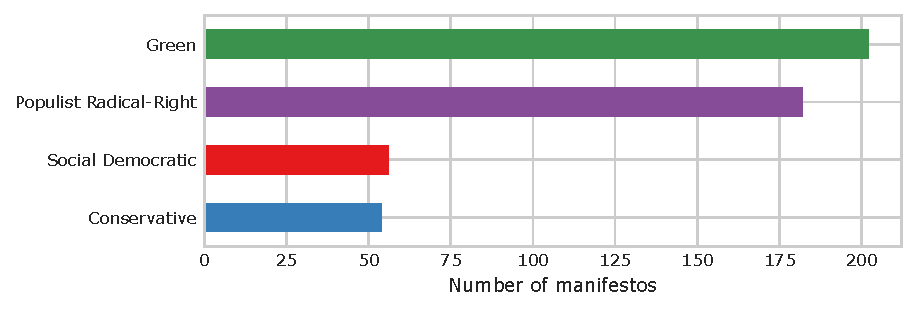
\includegraphics[keepaspectratio]{results/figures/figureA01.pdf}
  \caption{\label{figureA01}\protectNumber of manifestos by party family (all years).}
\end{figure}%

\begin{figure}[!th]
  \centering
  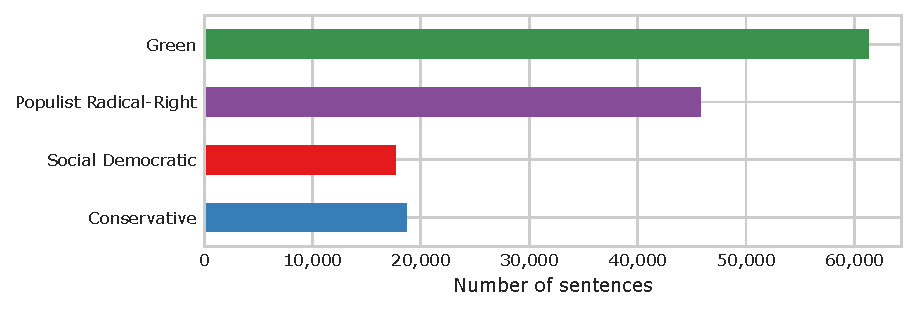
\includegraphics[keepaspectratio]{results/figures/figureA02.pdf}
  \caption{\label{figureA02}\protectNumber of sentences by party family (all years).}
\end{figure}%

\begin{figure}[!th]
  \centering
  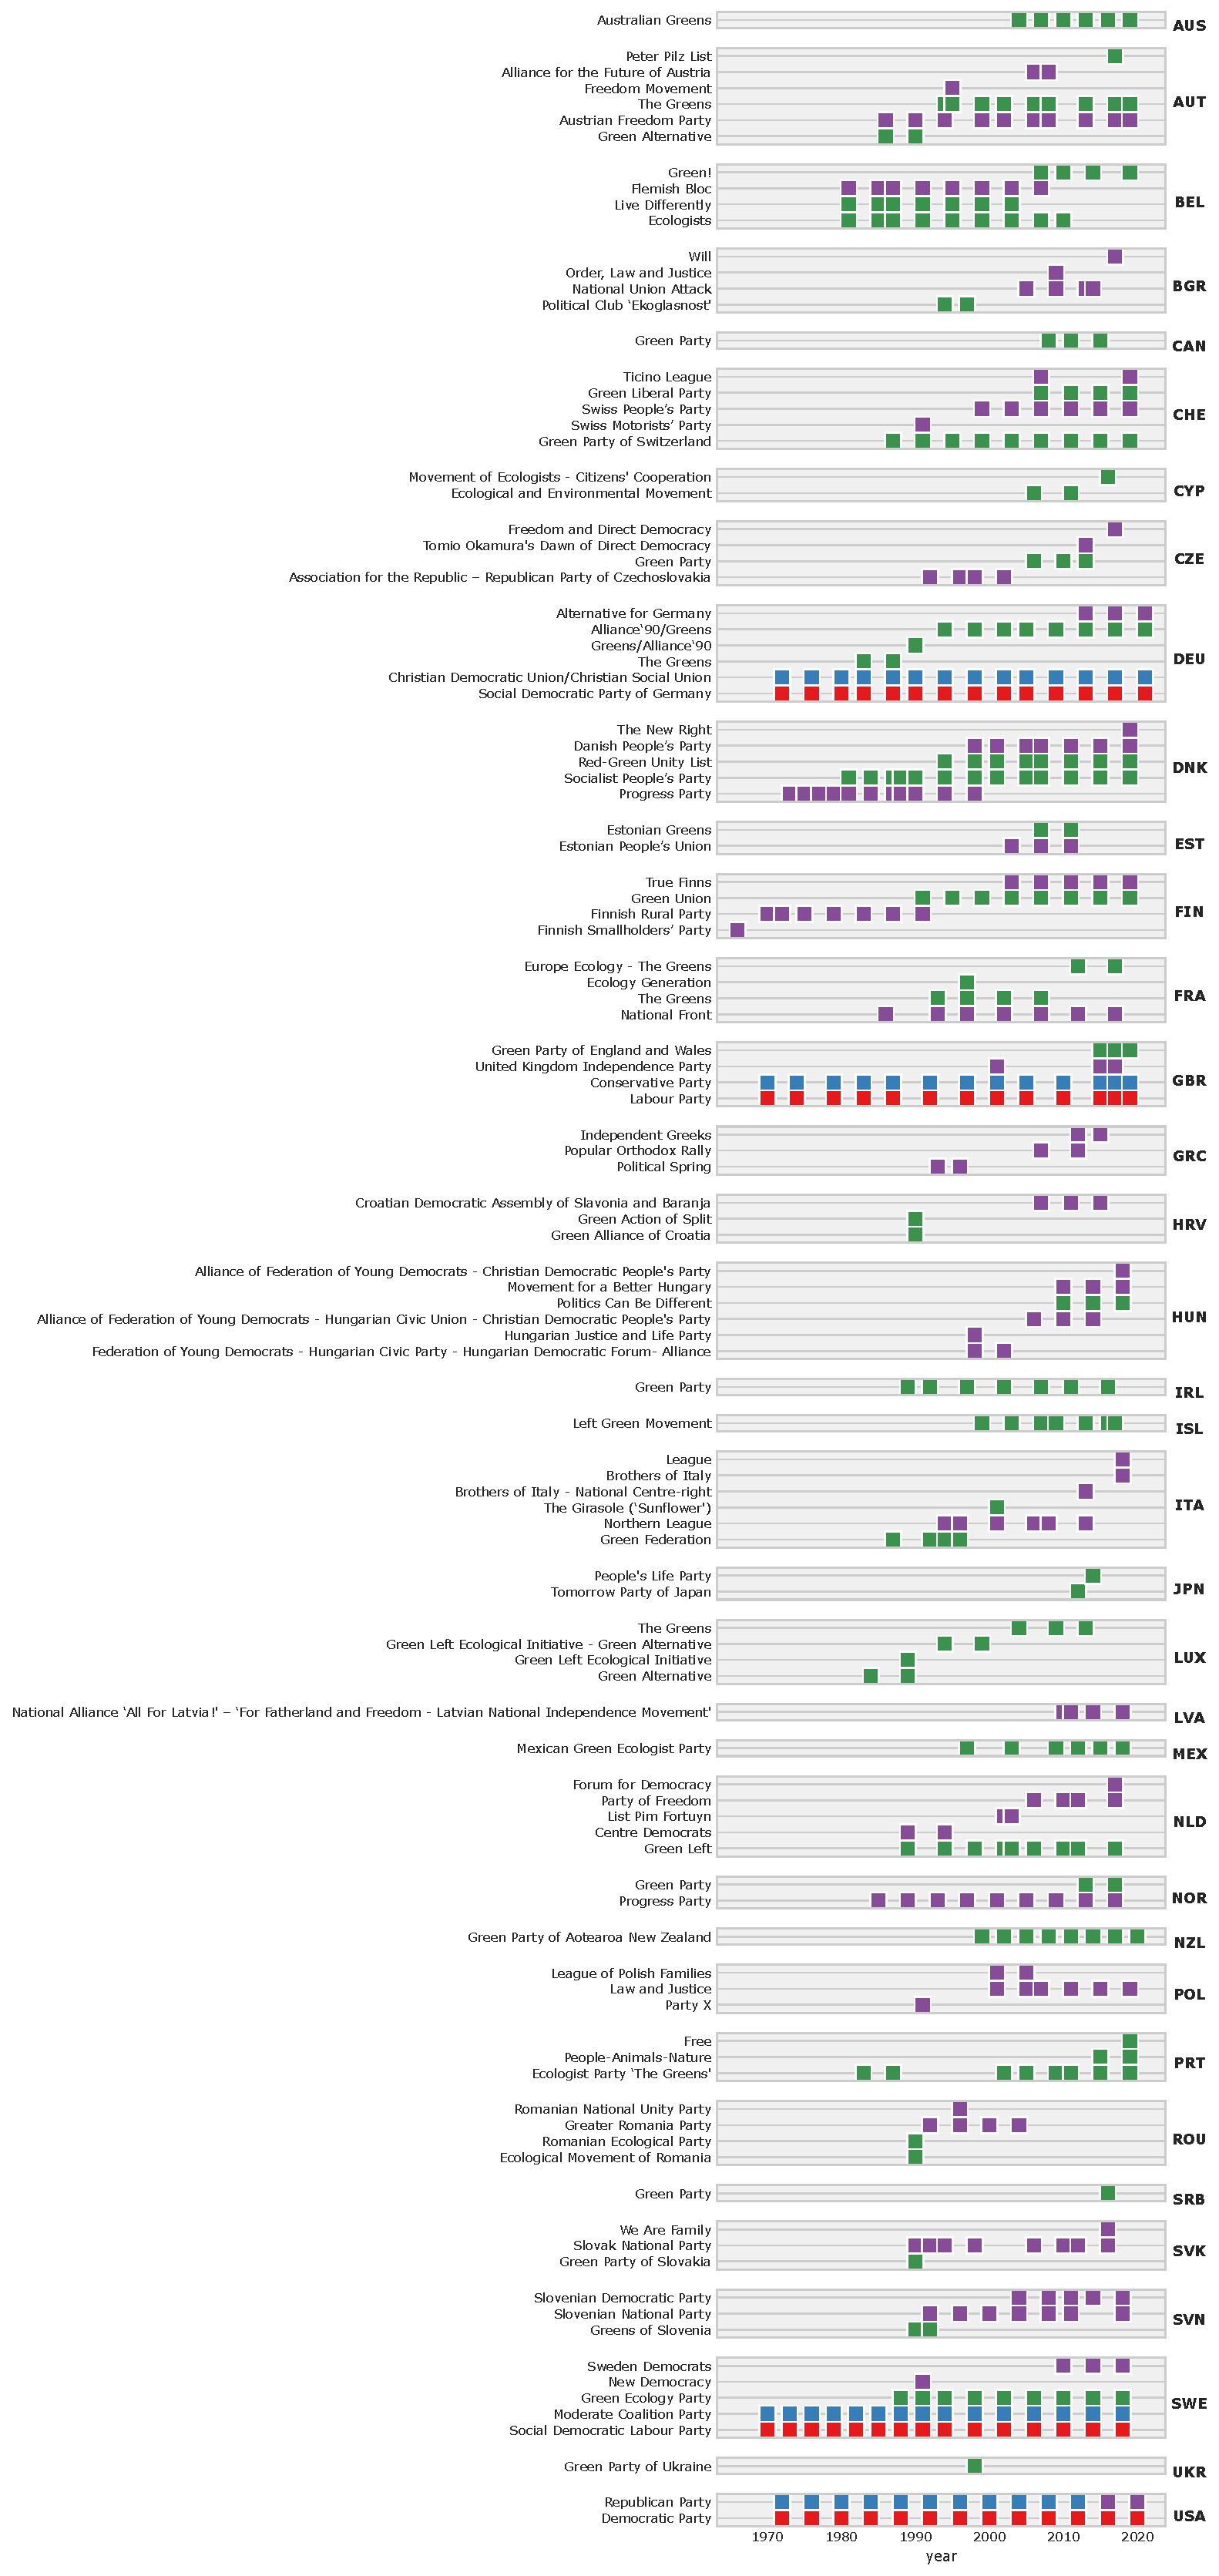
\includegraphics[keepaspectratio]{results/figures/figureA03.pdf}
  \caption{\label{figureA03}\protectOverview of cases included in our corpus. Each square represents a party in a given year, colored by its party family.}
\end{figure}%

\afterpage{
  \clearpage
  \thispagestyle{empty}
  \begin{figure}[p]
    \centering
    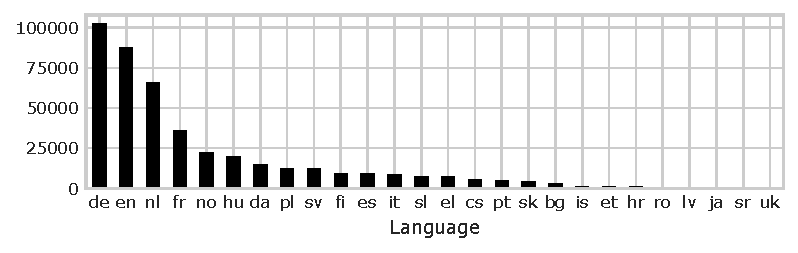
\includegraphics[keepaspectratio,width=\linewidth]{results/figures/figureA04.pdf}
    \caption{\label{figureA04}\protectLanguage coverage of the corpus of manifesto sentences. The corpus includes manifestos in 26 different languages. Languages denoted with their ISO 639-1 code. German (de), English (en), and Swedish (sv) are more strongly represented because our corpus also includes extensive time-series for social democratic and conservative parties in Germany, Sweden, the United Kingdom, and the United States. Other factors that contribute to languages' varying prevalence in our corpus are party system fragmentation and manifesto length, which, for example, explains the high number of Dutch (nl) sentences (many parties imply many manifestos).}
  \end{figure}%
  \clearpage
}

\clearpage

\section{Mention detection}\label{sec-apx_mention_detection}

Mention detection is the task of identifying which words or phrases in a sentence refer to social groups (Licht and Sczepanski 2025; Horne et al. 2025).
It is a prerequisite for classifying the attributes contained in social group mentions.

We produced the labeled data necessary for our application following the approach proposed by Licht and Sczepanski (2025), which combines sequence annotation (i.e., marking relevant phrases in sentences) and supervised token classification to extract any verbatim words or phrases used in a sentence to refer to social groups.

We proceeded in three annotation rounds, building on an active learning-like logic (cf. Miller et al. 2020) with the goal of maximizing the reliability and generalization of supervised classifiers trained on the collected annotations.
In the first round, we applied a informativeness-based sampling (Kaufman 2024) to maximally diversify the selection of examples distributed for annotation, selecting 4315 sentences for annotation (stratifying by manifesto, i.e., party and election).
To manually annotate social group mentions in this sample, we recruited a research assistant (RA) that already had experience with this annotation task from prior projects and proved very reliable.\footnote{In addition to being qualified for the task through prior experience, they received detailed coding instructions explaining the concept of social group mentions with definitions and examples and we performed two rounds of training with the RA using 231 and 238 sentences, respectively, sampled from our target corpus.
  This allowed us to assert the coder's ability to identify social group mentions in the target data and provide them with feedback.
}.

To prepare the second annotation round, we used the RA's annotations from round one to train a preliminary token classifier, applied it to the remaining sentences in our corpus, and computed classification uncertainty for each sentence based on the predicted probabilities of the preliminary classifier.
We then sampled 2473 sentences (again, stratifying by manifesto) with high prediction uncertainty for annotation for the second round.
Importantly, this sampling strategy allowed us to progressively focus the human annotation effort on difficult cases.

We repeated this process one more time -- annotation, classifier training, uncertainty-based sampling -- to sample another 988 sentences for annotation in a third round.

\begin{figure}[!th]
  \centering
  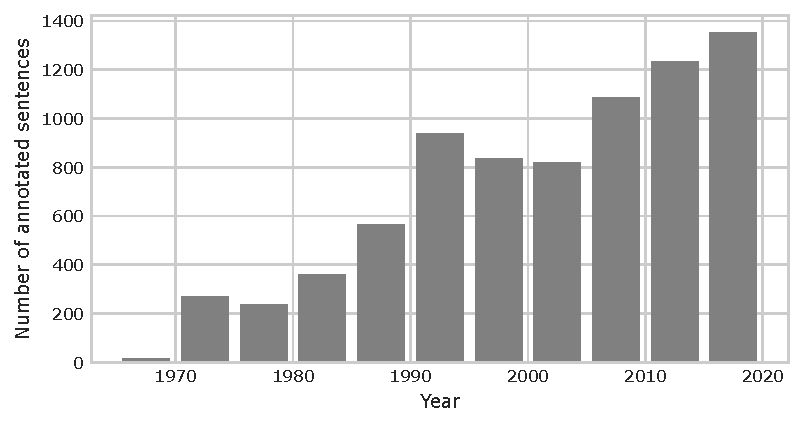
\includegraphics[keepaspectratio]{results/figures/figureB01.pdf}
  \caption{\label{figureB01}\protectDistribution of sentences annotated for group mention detection over time.}
\end{figure}%

Figure~\ref{figureB01} and Figure~\ref{figureB02} report the distribution of sentenes we annotated for group mentions across years and countries, respectively.
Both distribution reflects the coverage and composition of our manifesto corpus (see Figure~\ref{fig-cases_overview}) and the fact that we stratified by manifesto, not country or time, when sampling in our three annotation rounds.
This means that more fragmentized countries (e.g., Denmark) and/or counties with more elections are more strongly represented.
The alternative strategy of sampling equally across countries would, in contrast, have led to an underrepresentation of annotated examples from countries with many manifestos in our corpus.

Regarding the temporal distribution of our labeled sentences, it is notable that our data contains more sentences from manifestos from more recent decades.
This is because (a) Green and PRR parties only emerged gradually across the studied countries and (b) the missingness of manifesto raw texts tends to be comparatively higher in the 1970s and 1980s than in later decades.

Regarding the country distribution of annotated sentenecs, high-prevalence countries are those in which we have also covered a long time series of social democratic and conservative parties.
Moreover, Green and/or PRR parties were existing for longer periods in some countries, so that they feature more manifestos in our corpus, and hence have higher overall sampling rates throughout our annotation rounds.

\begin{figure}[!th]
  \centering
  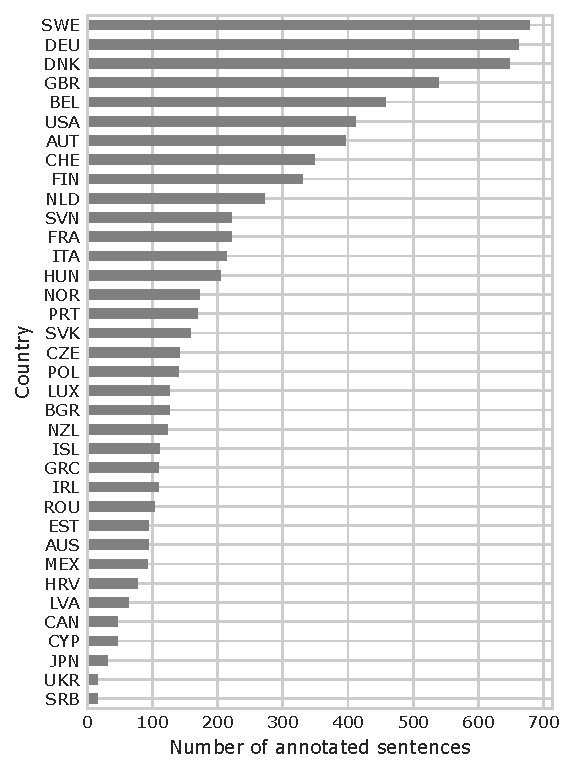
\includegraphics[keepaspectratio]{results/figures/figureB02.pdf}
  \caption{\label{figureB02}\protectDistribution of sentences annotated for group mention detection across countries.}
\end{figure}%


\clearpage

\section{Attribute classification}\label{sec-apx_attribute_classification}

\subsection{Coding instrument}\label{sec-coding_instrument}

Our coding instructions introduce the vertical/horizontal distinction, each of the attribute categories, as well as our ``universal'' group mention category, explain the available coding choices, and give examples.
Our coding instrument, implemented as a Qualtrix survey, presents annotators independently with one social group mention at a time (i.e., per page) in their respective sentence context, marking the mention in bold.

Below the display of the sentence, the annotator is first asked to indicate whether the highlighted mention is an ``universal'' mention per our definition.
If the annotator chose ``Yes'' for this coding dimension, our coding instructions asked them to proceed with the next instance on the next page.

If not, the annotator proceeds with coding the attribute categories for the vertical and horizontal attribute dimensions in turn.
For each of the dimensions, we tasked the annotator to indicate which of the respective attribute categories was contained in the highlighted social group mention, displaying the attribute categories below each other\footnote{We kept the categories' order fixed across examples to ease the cognitive load at annotation time.} in a multiple-choice grid with the answer options ``Yes'' or ``Unsure'' horizontally aligned.\footnote{We omitted options for ``No'' because not choosing ``Yes'' or ``Unsure'' for a given attribute category implied this coding choice.}
This procedure results in 17 annotations\footnote{1\(\times\) universal + 5\(\times\) vertical attributes + 11\(\times\) horizontal attributes} per mention-in-sentence-context instance and annotator.

\subsection{Annotation}\label{annotation-1}

In a first round of annotations, we have sampled 300 mentions-in-sentence-context examples from all sentences with at least one predicted social group mention, again using an informativeness-based sampling strategy.
Table~\ref{tableC01} reports the micro inter-annotator agreement (ICA) by attribute dimension from this round and indicated that our coders produced overall reliable annotations.
To resolve examples with disagreeing annotations, the authors team reviewed any mention-in-sentence-context example with at least one disagreeing annotation to determine their final labels.

However, as expected, the prevalence of attribute categories in the labels collected in this first round turned out to be very imbalanced and we observed variation in ICA estimates across categories that could only partially be explained by low prevalence (see Table~\ref{tableC02}).
We therefore dedicated a second annotation round to collecting more annotations for difficult examples.
To this end, we fine-tuned a multilabel classifier to predict mentions-in-sentence-context examples' binary labels on the universal, vertical, horizontal indicators based on the consolidated annotations collected in the first round.
We applied this classifier to the mention-in-sentence-context instances not yet distributed for attribute annotation to obtain predicted probabilities.
We then computed classification uncertainty at the example level and selected the 150 most uncertain examples into a second annotation batch.

Table~\ref{tableC01} and Table~\ref{tableC02} show that, due to our focus on difficult examples, ICA was generally lower than in the first round.
We therefore used zero-shot in-context learning (Brown et al. 2020) to generate large language model (LLM) annotations for the examples in the second-round batch.
We then presented our annotators the instances where the LLM disagreed with their judgment and tasked them to (independently) judge which annotation they viewed as more valid while blinding them towards the source of the respective annotations.
The author team arbitrated the cases in which our annotators' independent judgments disagreed.
All instances from this second round were then consolidated into final labels and added to those of the first round.

\begin{table}[!th]
\centering
\caption{Inter-coder agreement estimates for attribute classifications computed at the level of attribute dimensions: universal, economic, and non-economic. Estimates are based on Krippendorff's $\alpha$ and the prevalence of `yes' annotations (prevalence) across all annotated examples in each annotation round.}
\label{tableC01}
\begin{tabular}{rrrrrrr}
\toprule
 & \multicolumn{3}{c}{Krippendorff's $\alpha$} & \multicolumn{3}{c}{prevalence} \\
annotation round & 1 & 2 & 3 & 1 & 2 & 3 \\
\midrule
universal & 0.697 & 0.259 & 0.000 & 0.275 & 0.144 & 0.006 \\
economic & 0.791 & 0.731 & 0.806 & 0.410 & 0.687 & 0.318 \\
non-economic & 0.754 & 0.474 & 0.752 & 0.563 & 0.727 & 0.844 \\
\bottomrule
\end{tabular}
\end{table}
%

\begin{table}[!th]
\centering
\caption{Inter-coder agreement estimates for attribute classifications computed at the level of economic and non-economic attribute categories. Estimates are based on Krippendorff's $\alpha$ and values in parentheses indicate the prevalence of `yes' annotations (prevalence) across all annotated examples in each annotation round.}
\label{tableC02}
\resizebox{\textwidth}{!}{%
\begin{tabular}{rrrrr}
\toprule
 & annotation round & 1 & 2 & 3 \\
dimension & category &  &  &  \\
\midrule
\multirow[t]{4}{*}{economic} & education & +0.799 (1.0\%) & +0.847 (8.0\%) & +0.888 (8.9\%) \\
 & employment status & +0.527 (8.8\%) & +0.607 (12.8\%) & +0.650 (6.7\%) \\
 & income/wealth/economic status & +0.694 (6.9\%) & +0.903 (13.0\%) & +0.745 (2.8\%) \\
 & occupation/profession & +0.804 (18.7\%) & +0.694 (28.8\%) & +0.241 (12.9\%) \\
\cmidrule(lr){1-5}
\multirow[t]{10}{*}{non-economic} & age & +0.832 (17.5\%) & +0.704 (12.8\%) & +0.442 (10.7\%) \\
 & crime & +0.659 (3.4\%) & +0.847 (8.0\%) & +0.842 (11.2\%) \\
 & ethnicity & +0.664 (1.3\%) & +0.658 (4.0\%) & +0.822 (25.1\%) \\
 & family & +0.765 (8.4\%) & +0.650 (6.7\%) & +0.753 (10.7\%) \\
 & gender/sexuality & +0.830 (2.4\%) & -0.021 (4.7\%) & +0.842 (25.8\%) \\
 & health & +0.906 (4.0\%) & +0.359 (10.7\%) & +0.607 (15.3\%) \\
 & nationality & +0.804 (12.9\%) & +0.581 (16.0\%) & +0.443 (20.8\%) \\
 & place/location & +0.662 (2.0\%) & +0.854 (2.7\%) & +0.496 (1.7\%) \\
 & religion & +0.666 (0.7\%) & +0.322 (3.3\%) & +0.959 (16.8\%) \\
 & shared values/mentalities &  & +0.567 (23.4\%) & +0.484 (5.0\%) \\
\bottomrule
\end{tabular}
}%
\end{table}
%

In a third round of annotation, we then addressed the problem of label class imbalance that clearly showed in the pooled set of multi-labeled mention-in-sentence-context instances from rounds one and two.
In particular, we focused on over-sampling likely examples of so far under-represented attribute categories in the vertical and horizontal attribute dimensions.
To identify likely examples for the given label categories, we used the attribute category definitions to define queries and used a pre-trained sentence embedding model to rank so far unannotated mention-in-sentence-context instances based on their cosine similarities to each of these queries.
To oversample likely examples of so far underrepresented categories, we defined quotas for each attribute category in inverse proportion to the categories prevalence in the labeled instances from round one and two, using a annotation budget of 200 examples for round 3.
We then chose as many of the so far unanottated mention-in-sentence-context instances as the quote prescribed in descending order of their embeddings' similarities to the embedding of the respective attribute category definition query.
In total, this resulted in a samole of 180 mention-in-sentence-context examples for annotation in round 3.\footnote{Deviations from the annotation budget of 200 cases are explained by rounding in the computation of quotas and some mention-in-sentence-context instances that were ranked high for multiple attribute queries.}

Table~\ref{tableC01} shows that the attribute annotations of examples in this third round were overall highly reliable, which is likely explained by focusing on identifying \emph{likely} examples of each attribute category in this final round (in contrast to difficult instances in round 2).
Further, the consolidated labels from round 3 showed that our over-sampling strategy was effective as it helped to reduce the label class imbalance across the set of vertical and horizontal attribute categories.

A last round of annotation focused on conceptual consolidation and was performed by the authors.
Specifically, we manually reviewed any annotated examples that were labeled as combining certain attribute categories to determine whether the combination of these categories was conceptually valid and consistent with our attribute definitions.

\subsection{SetFit fine-tuning}\label{sec-apx_setfit}

Tunstall et al. (2022) propose a sentence transformer fine-tuning (SetFit) approach for few-shot learning in text classification applications.
In this framework, labeled examples in the training set are first used to construct pairs for contrastive embedding model fine-tuning.
This specializes a general-purpose sentence embedding model for representing social group mentions.
The contrastive finetuning task in the embedding finetuning step practically augments our 600 annotated examples to several thousand contrastive pairs, thus providing ample training material for embedding model finetuning.
This already effectively tunes the text representations that go into the attribute category multilabel classification head to our target concept.

Second, the fine-tuned embeddings are input to a classification head.
The classification head is the component that maps a mentions embedding into a multilabel attribute classification.
Both components are trained end-to-end for multilabel classification on labeled examples.

\subsubsection{Data splitting}\label{data-splitting}

We have first carefully split the 600 annotated examples into five training, validation and test folds to minimize leakage between the training and evaluation sets.
This is generally a crucial step in any supervised machine learning application, but it is particularly important in our application for several reasons.
First, simple random sampling does not account for the facts that
(a) mentions are embedded in sentences so that the same mention can appear in multiple sentences and
(b) some mentions are near duplicates of each other and having these in different splits can lead to overestimation of predictive performance.
Second, in the context of few-shot learning, it is particularly important to minimize leakage between the training and evaluation sets because the small number of training examples makes it more likely that a given example in the evaluation set is very similar to one in the training set, which can lead to overestimation of predictive performance.

\subsubsection{Evaluating implementation choices}\label{evaluating-implementation-choices}

We have thoroughly evaluated several implementation choices such as the base embedding model,\footnote{We evaluated models of varying size and architecture, including
  \href{https://huggingface.co/sentence-transformers/all-MiniLM-L6-v2}{\texttt{all-MiniLM-L6-v2}},
  \href{https://huggingface.co/sentence-transformers/all-mpnet-base-v2}{\texttt{all-mpnet-base-v2}},
  \href{https://huggingface.co/Alibaba-NLP/gte-modernbert-base}{\texttt{gte-modernbert-base}},
  \href{https://huggingface.co/nomic-ai/modernbert-embed-base}{\texttt{modernbert-embed-base}},
  \href{https://huggingface.co/ibm-granite/granite-embedding-english-r2}{\texttt{granite-embedding-english-r2}},
  \href{https://huggingface.co/google/embeddinggemma-300m}{\texttt{embeddinggemma-300m}},
  and
  \href{https://huggingface.co/Qwen/Qwen3-Embedding-0.6B}{\texttt{Qwen3-Embedding-0.6B}}} input formatting strategy,\footnote{We evaluated inputting only the groupmention text, concatenating the mention text with its sentence context (pre- vs.~suffixing), and a custom span embedding strategy that pools the token embeddings of the mention text from the last layer of the embedding model.} and hyperparameter choices.

We have then used the training and validation split to examine the average performance of different base embedding models\footnote{We evaluated models of varying size and architecture, including
  \href{https://huggingface.co/sentence-transformers/all-MiniLM-L6-v2}{\texttt{all-MiniLM-L6-v2}},
  \href{https://huggingface.co/sentence-transformers/all-mpnet-base-v2}{\texttt{all-mpnet-base-v2}},
  \href{https://huggingface.co/Alibaba-NLP/gte-modernbert-base}{\texttt{gte-modernbert-base}},
  \href{https://huggingface.co/nomic-ai/modernbert-embed-base}{\texttt{modernbert-embed-base}},
  \href{https://huggingface.co/ibm-granite/granite-embedding-english-r2}{\texttt{granite-embedding-english-r2}},
  \href{https://huggingface.co/google/embeddinggemma-300m}{\texttt{embeddinggemma-300m}},
  and
  \href{https://huggingface.co/Qwen/Qwen3-Embedding-0.6B}{\texttt{Qwen3-Embedding-0.6B}}} and input formatting strategies\footnote{We evaluated inputting only the mention text, concatenating the mention text with its sentence context (pre- vs.~suffixing), and a custom span embedding strategy that pools the token embeddings of the mention text from the last layer of the embedding model.} and select the best-performing model and formatting strategy for each classifier.
Finally, we have trained the two classifiers on the full training set using the selected embedding model and input formatting strategy and evaluated their performance on the held-out test set.

\subsection{Validation}\label{sec-apx_validity}

\subsubsection{Content validity}\label{content-validity}

Besides their reliability, we also need to assess whether our classifier categorizes social group mentions in a substantively meaningful way.
We do so by analyzing the lexical patterns that characterize social group mentions assigned into our different attribute categories.
Specifically, we apply the ``fighting words'' bag-of-words method (Monroe et al. 2008) for identifying distinctive terms to quantify which terms are most strongly associated with our attribute categories.
 If our classifiers capture the attribute categories we conceptualize, their most distinctive terms should align with our substantive priors.

To enable this analysis, we have used our attribute classifiers to annotate all social group mentions extracted by our group mention detection model in our manifesto sentences corpus.
Note that we also include the manifestos of centre-left and -right parties covered by our case selection strategy in this validity assessment.

\paragraph{Universal group mentions}\label{universal-group-mentions}

\begin{figure}[!th]
  \centering
  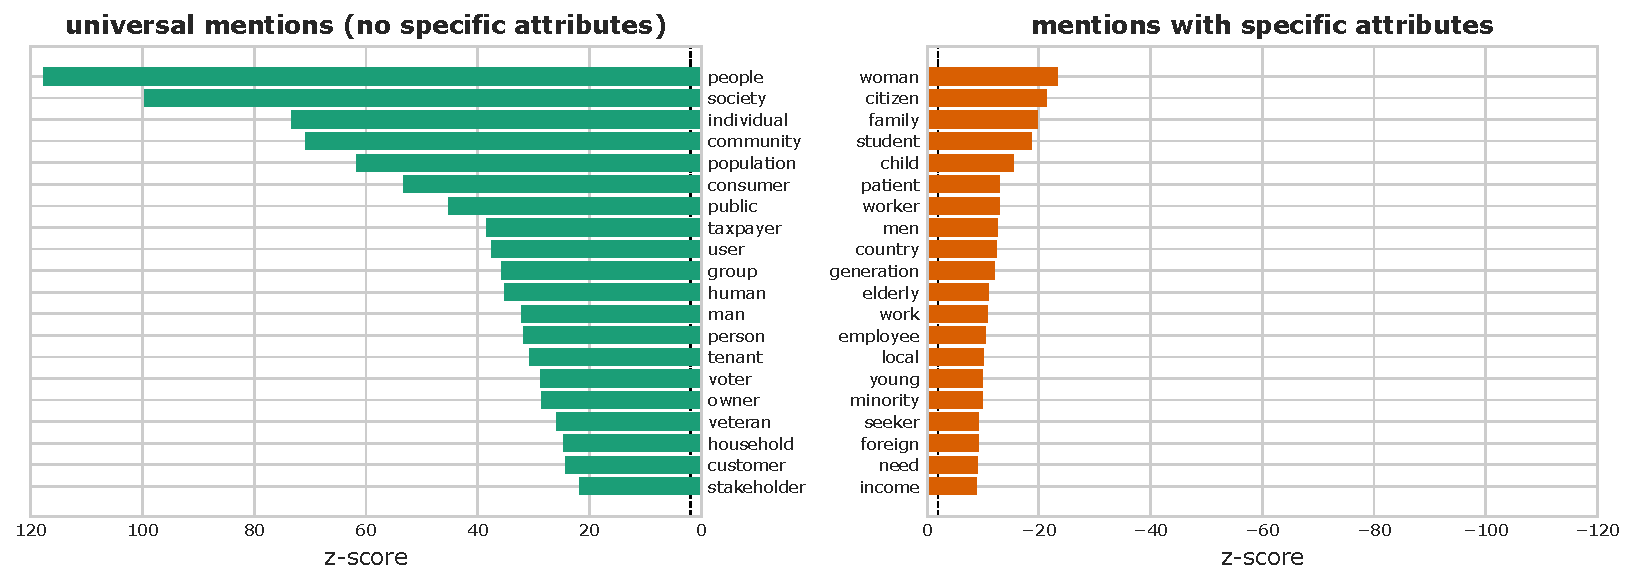
\includegraphics[keepaspectratio,width=\linewidth]{results/figures/figureC01.pdf}
  \caption{\label{figureC01}\protectMost distinctive words for mentions with no specific attributes (\emph{universal} mentions, left) vs. mentions with at least one economic or non-economic attribute (right).  Values plotted are $z$-scores from ``fighting words'' analysis.  Values above ±1.96 (vertical dashed line) can be considered significantly distinctive.}
\end{figure}%

We consider predicted group mentions that are predicted to contain no attributes as ``universal'' group references, that is, references to groups in general without specifying which kind of people they mean exactly.
To validate, that the predicted absence of attributes in these mentions indeed reflects this conceptual category, we examine the most distinctive \(n\)-grams of these mentions by applying the ``fighting words'' method (Monroe et al. 2008) to all group mentions in our corpus, using a binary indicator of whether a mention is predicted to be a ``universal'' group reference as grouping variable.\footnote{We have split mentions into tokens, removed English stop words, lemmatized tokens, computed uni-, bi-, and trigrams, and discarded any tokens that occurred in more than 80\% of mentions or in less than 5 mentions.}

Figure~\ref{figureC01} shows the top 20 most distinctive \(n\)-grams of ``universal'' group references.
The set of most distinctively ``universal'' terms includes tokens like ``people'', ``society'', ``everyone'', and similar terms that are used as generic collectivisms in the English language.
The most distinctively non-``universal'' terms, in turn, include denotational group labels like ``women'', ``students'', ``citizens'', and ``family''.

\paragraph{Attribute categories}\label{attribute-categories-1}

For the fighting words analysis of our attribute categories, we have first subset the dataset of extracted and labeled social group mentions to ``non-universal'' group mentions, that is, mentions that were classified as featuring at least one attribute covered by our taxonomy. For each attribute category, we have then estimated the fighting words \(z\)-scores that measure distinctiveness by contrasting mentions that are predicted to feature the given attribute with those that are predicted to not feature it.

\afterpage{%
  \clearpage%
  \thispagestyle{empty}%
  \begin{landscape}%
  \begin{table}[!th]
\centering
\caption{Most distinctive terms for each attribute category, based on the ten tokens with the highest fighting words $z$-scores. The $z$-scores, reported in parentheses, indicate how strongly a term is associated with mentions in that attribute category compared to social group mentions that do feature attributes from this category. \emph{Note:} See \ref{figureC02} and \ref{figureC03} for visual presentations of the data.}
\label{tableC03}
\begin{tabular}{lp{0.2\textwidth}p{0.9\textwidth}}
\toprule
 &  & top-10 most distinctiveterms \\
\midrule
\multirow[t]{4}{*}{economic} & education & student~(71.9), school~(47.4), education~(42.6), senior~(31.2), training~(25.0), pupil~(24.7), higher~(23.4), university~(23.1), study~(21.0), higher education~(19.8) \\
 & employment status & worker~(97.9), employee~(71.1), work~(49.7), working~(49.1), job~(35.0), workforce~(32.4), pensioner~(30.9), staff~(30.2), unemployed~(27.7), employed~(25.4) \\
 & income/wealth/economic status & need~(42.5), income~(35.8), group~(33.6), vulnerable~(32.4), low~(30.0), household~(29.6), class~(28.7), poor~(28.2), disadvantaged~(25.7), middle~(25.3) \\
 & occupation/profession & member~(39.1), public~(33.8), professional~(32.7), official~(26.5), representative~(26.0), personnel~(25.2), police~(23.8), politician~(23.2), health~(22.0), leader~(21.9) \\
\cmidrule(lr){1-3}
\multirow[t]{10}{*}{noneconomic} & age & child~(131.2), people~(59.0), young~(55.7), elderly~(36.7), future~(35.5), youth~(35.0), age~(34.6), generation~(34.5), year~(27.0), adult~(25.8) \\
 & crime & victim~(51.8), criminal~(47.6), violence~(30.0), drug~(28.2), prisoner~(28.1), crime~(27.5), prison~(23.6), sexual~(20.8), abuse~(20.7), terrorist~(20.5) \\
 & ethnicity & minority~(67.0), ethnic~(28.7), group~(26.3), black~(24.7), islander~(22.4), diverse~(20.3), national minority~(19.4), religious~(19.2), torres~(19.1), torres strait~(19.1) \\
 & family & child~(124.3), family~(71.4), parent~(31.6), single~(26.8), relative~(25.3), spouse~(24.5), caregiver~(20.9), couple~(18.1), mother~(17.7), family member~(16.4) \\
 & gender/sexuality & woman~(113.9), men~(72.5), couple~(27.6), girl~(27.2), sexual~(18.8), boy~(18.8), sex~(18.2), young woman~(15.5), mother~(15.1), position~(14.2) \\
 & health & person~(45.2), patient~(41.2), need~(39.2), people~(38.4), care~(34.6), vulnerable~(33.5), disabled~(30.7), affected~(27.2), sick~(25.7), special~(25.2) \\
 & nationality & citizen~(69.5), country~(42.8), american~(36.9), seeker~(30.5), nation~(26.6), national~(26.5), resident~(23.1), european~(22.9), foreign~(22.0), asylum~(21.4) \\
 & place/location & community~(58.7), local~(55.6), country~(49.9), resident~(44.8), rural~(35.4), living~(35.1), population~(29.4), germany~(28.0), area~(27.3), inhabitant~(26.5) \\
 & religion & community~(26.4), religious~(26.3), ethnic~(25.5), minority~(22.9), christian~(19.9), muslim~(19.2), faith~(18.8), multicultural~(17.6), different~(17.0), islamic~(16.9) \\
 & shared values/mentalities & society~(98.1), want~(38.3), free~(27.4), right~(27.2), life~(23.8), civil~(22.0), human~(20.9), democratic~(20.8), value~(19.5), green~(19.0) \\
\bottomrule
\end{tabular}
\end{table}
%
  \end{landscape}%
  %\clearpage%
}%

Table~\ref{tableC03} reports the top-10 tokens for each attribute category in our taxonomy resulting from this analysis.
Overall, the most distinctive terms strongly align with our expectations of the valid content of these categories.
For example, the most distinctive tokens for the economic attribute category \emph{education} are a semantically highly coherent cluster of terms related to groups (``students'' and ``pupils'') and contexts related to education (``school'', ``university'', and ``training'').
And for our novel \emph{shared values/mentalities} category, the most distinctive tokens feature many value-based adjectives and the lemmas of ``society'', which stands out because value-based group references tend to center on parties' visions of a society with certain shared values.
We view these results as strong evidence of the content validity of our classifiers.

\begin{figure}[!th]
  \centering
  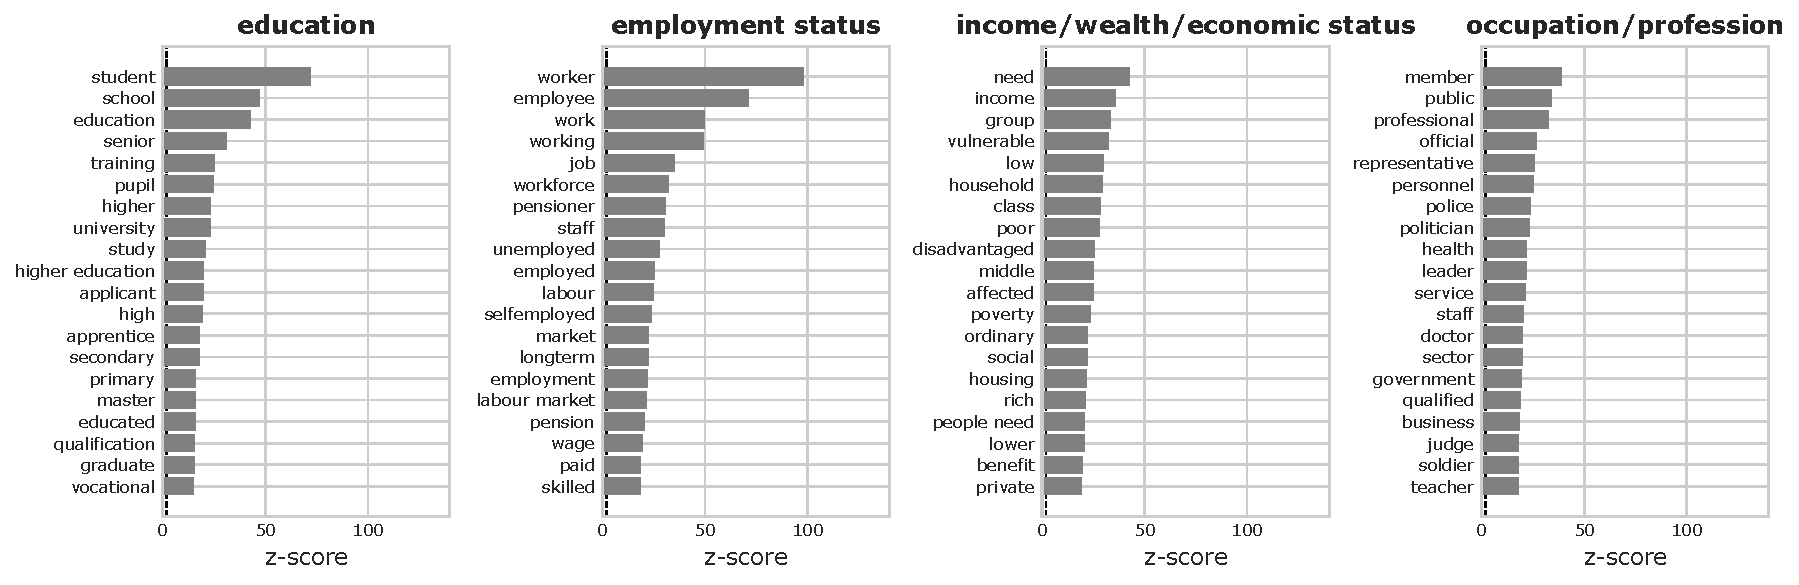
\includegraphics[keepaspectratio,width=\linewidth]{results/figures/figureC02.pdf}
  \caption{\label{figureC02}\protectMost distinctive words of social group mentions categorized as featuring a specific economic attribute. Values plotted are $z$-scores from ``fighting words'' analysis computed for mentions in focal category vs. all other non-universal mentions. Values above ±1.96 (vertical dashed line) can be considered significantly distinctive.}
\end{figure}%

\begin{figure}[!th]
  \centering
  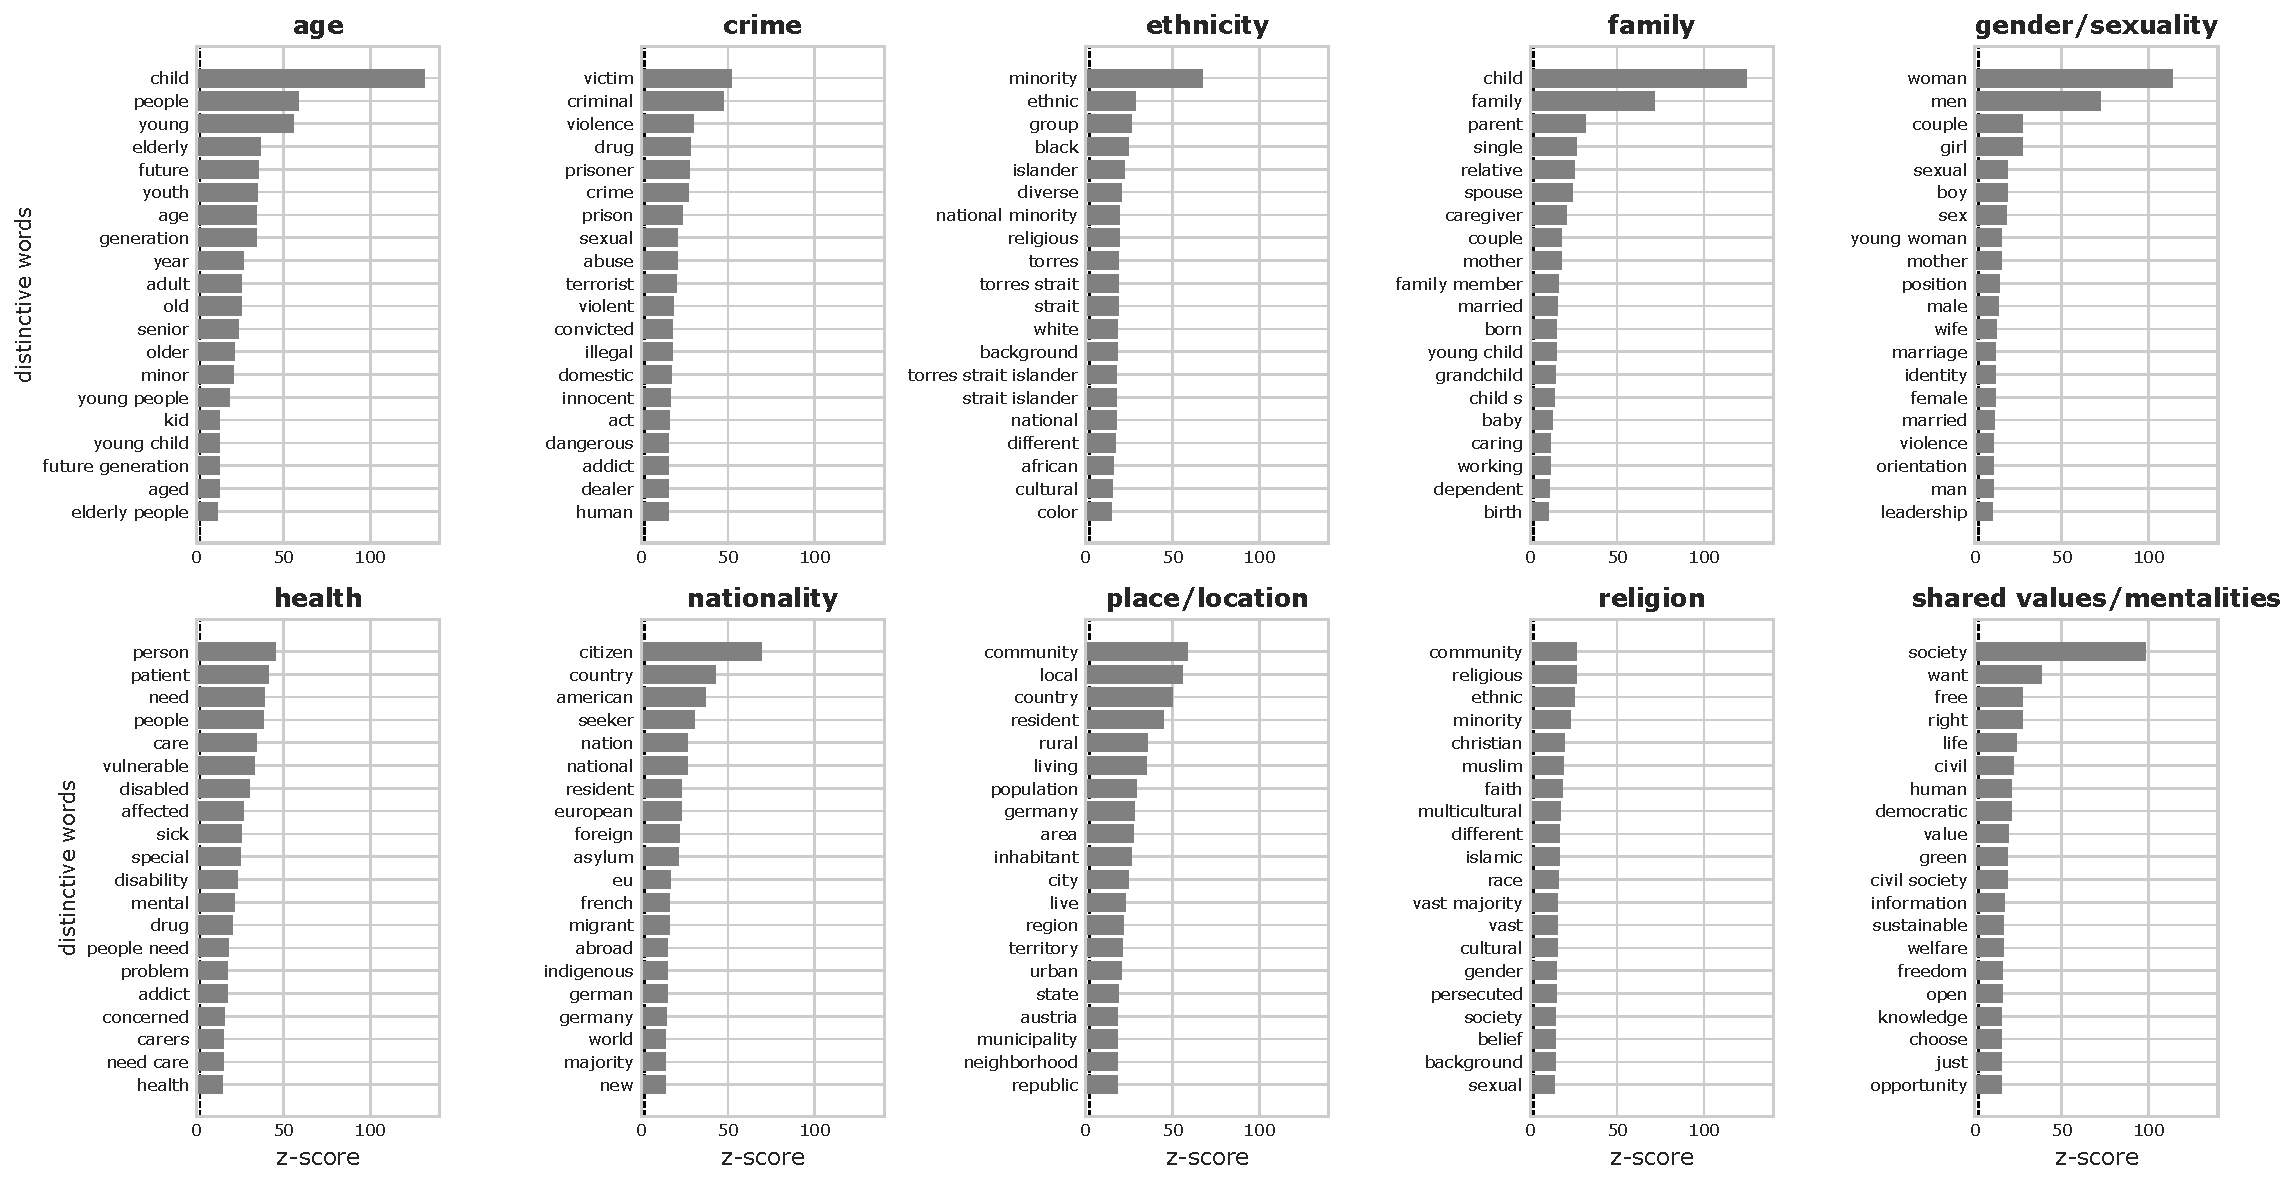
\includegraphics[keepaspectratio,width=\linewidth]{results/figures/figureC03.pdf}
  \caption{\label{figureC03}\protectMost distinctive words for social group mentions categorized as featuring a specific non-economic attribute. Values plotted are $z$-scores from ``fighting words'' analysis computed for mentions in focal category vs. all other non-universal mentions. Values above ±1.96 (vertical dashed line) can be considered significantly distinctive.}
\end{figure}%

The clarity of the top terms raises the question of whether the mention-level attribute classification could as well be achieved with a set of rather simple dictionaries.
Additional analysis reported in Table~\ref{tableC04} speak against this simple alternative for most attribute categories.
While in the case of attribute categories like \emph{family}, \emph{age}, \emph{employment status} or \emph{education}, between 88\% and 70\% of mentions classified as featuring an attribute of the respective category also contain one of the top-10 terms of this category shown in Table~\ref{tableC03}, this estimate of recall of the top-10 terms is much lower for categories like \emph{religion} (42\%), \emph{nationality} (36\%), \emph{income/wealth/economic status} (33\%) or \emph{occupation/profession} (20\%).\footnote{Increasing the number of top terms to 40 or 50 only mitigates this partially with diminishing returns.} The latter group of categories thus seem to be centered on clear semantic clusters; our classifiers are able to capture them relatively reliably but the small sets of most-distinctive lexical features are not.
This conjuncture is supported by the qualitative insights we gained during annotations as well as the overall lower magnitude of the \(z\)-scores for these categories.
In sum, while indicating the high content validity of our classifiers, the most distinctive terms alone do not fully capture the essence of mentions in the respective attribute categories.

\begin{table}[!th]
\centering
\caption{Performance of the top $k$ terms for each attribute category in predicting the presence of that attribute in mentions. The table reports the proportion of mentions in each attribute category that contain at least one of the top $k$ terms for that category. The top $k$ terms are determined based on the ten tokens with the highest fighting words $z$-scores.}
\label{tableC04}
\begin{tabular}{rrrrrrr}
\toprule
 &  & \multicolumn{5}{c}{top $k$ terms} \\
 &  & 10 & 20 & 30 & 40 & 50 \\
\midrule
\multirow[t]{4}{*}{economic} & employment status & 0.793 & 0.830 & 0.852 & 0.878 & 0.889 \\
 & education & 0.701 & 0.780 & 0.817 & 0.837 & 0.849 \\
 & income/wealth/economic status & 0.329 & 0.446 & 0.527 & 0.585 & 0.613 \\
 & occupation/profession & 0.200 & 0.362 & 0.412 & 0.464 & 0.534 \\
\cmidrule(lr){1-7}
\multirow[t]{10}{*}{noneconomic} & family & 0.883 & 0.894 & 0.910 & 0.916 & 0.918 \\
 & age & 0.843 & 0.888 & 0.895 & 0.905 & 0.910 \\
 & gender/sexuality & 0.809 & 0.837 & 0.850 & 0.871 & 0.872 \\
 & health & 0.742 & 0.848 & 0.877 & 0.895 & 0.903 \\
 & ethnicity & 0.609 & 0.690 & 0.768 & 0.803 & 0.810 \\
 & place/location & 0.538 & 0.622 & 0.666 & 0.678 & 0.684 \\
 & shared values/mentalities & 0.486 & 0.512 & 0.555 & 0.592 & 0.620 \\
 & crime & 0.476 & 0.539 & 0.683 & 0.713 & 0.733 \\
 & religion & 0.420 & 0.501 & 0.533 & 0.538 & 0.542 \\
 & nationality & 0.367 & 0.411 & 0.421 & 0.507 & 0.513 \\
\bottomrule
\end{tabular}
\end{table}
%

\clearpage

\subsubsection{Comparison to other categorization schemes}\label{sec-convergence}

To further validate our attribute-centered social group mention classification approach, we compare the classifications produced with our scheme and classifiers with those produced by two existing \emph{group} categorization schemes developed by Thau (2019) and Horne et al. (2025), respectively.
This analysis shows both alignment and key differences between the schemes, highlighting the added analytical value of our attribute-centered approach, that takes attribute combinations and varying levels of abstraction into account.

\paragraph{Comparison to Thau's social group category classifications}\label{sec-thau_crossvalidation}

Thau (2019) has the analytical goal in common with our study.
He focuses on identifying \emph{and} classifying group mentions in the party manifestos of the British \emph{Labour} and \emph{Conservative} parties {[}1964-2015; cf. Thau (2021){]} -- cases also covered by our corpus and samples of human-annotated texts.
He has developed a group categorization scheme that differentiates between five group types, including the types \emph{Social group} and \emph{Professional group}.
Within \emph{Social group} mentions, he further distinguishes between nine group categories.

However, a critical distinction between Thau's and our approach is that he assigns each group mention that his annotators identified to one and only one social group category.
In contrast, our taxonomy and classifiers account for the logic of attribute combination by allowing each mention to be assigned to multiple attribute categories.
This overlap in case coverage and analytical goal but difference in measurement strategy allows us to directly clarify the added value of multi-label attribute classification of our approach.

To compare our approach to Thau's group category annotations, we have applied our classifiers to the 4,018 human-labeled social and professional group mentions examples in his annotated data.\footnote{Our corpus and samples of human-annotated texts also include \emph{Labour} and \emph{Conservative} party manifestos, making this an in-sample analysis.} This allows us not only to analyze both how our attribute-centered classification aligns with his group categories.
It also enables us to analyze how often our different attribute categories have been assigned to group mentions grouped into one group category in Thau's scheme, thus offering insights into what might have been lost in annotation by forcing single-class assignments.

\begin{figure}[!th]
  \centering
  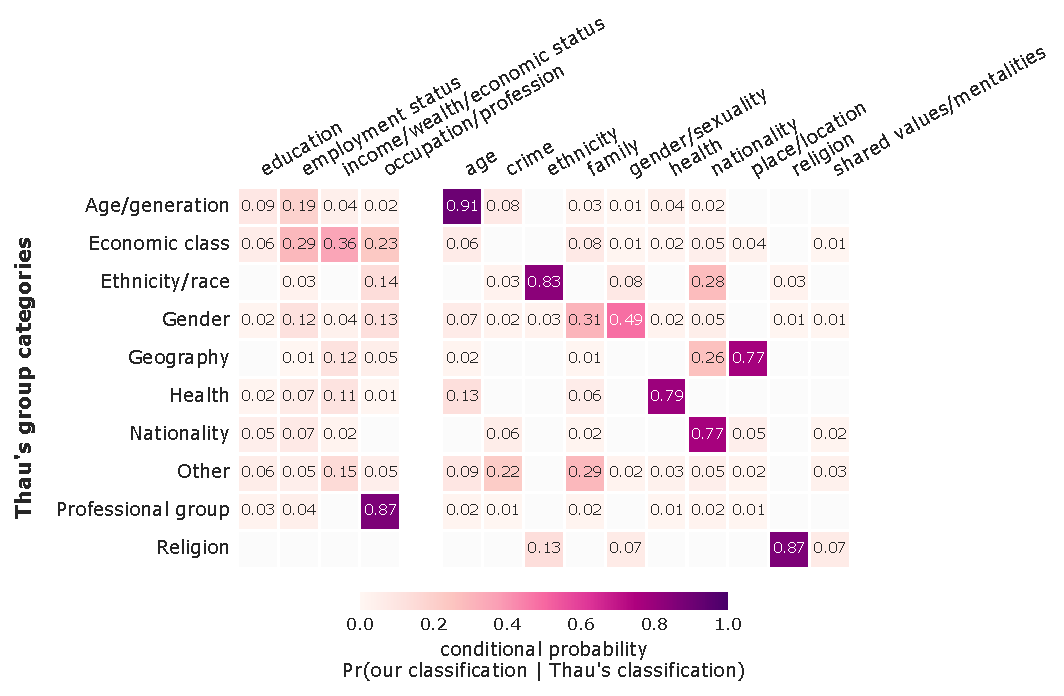
\includegraphics[keepaspectratio]{results/figures/figureC04.pdf}
  \caption{\label{figureC04}\protectCorrespondence of Thau's social group categorizations with our group attribute classifications. Numbers report the probability that a mention assigned by Thau's coders to one of his social group categories (shown on y-axis) has been labeled as featuring a given social attribute in our classification scheme (shown on x-axis). \emph{Note:} Values below 0.009 not plotted to ease readability.}
\end{figure}%

Figure~\ref{figureC04} shows the results of this analysis  by reporting the probability that our classifiers label a mention with an attribute (x-axis), given the mentions' categorization in Thau's data (y-axis).
On the one hand, this shows strong correspondence between some of Thau's group categories and our attribute categories.
For example, 91\% of Thau's \emph{Age/generation} mentions are labeled as \emph{age} by our classifier, 83\% of mentions in his \emph{Ethnicity/race} category are labeled as \emph{ethnicity} by our classifier, and 87\% of group mentions in his \emph{Professional group} category are also classified as featuring an \emph{occupation/profession}-related attribute by our classifiers.

However, Figure~\ref{figureC04} also shows diversity within the mentions that Thau's annotators have assigned to only one of the group categories in his schemes.
For example, while 91\% of Thau's \emph{Age/generation} mentions are labeled as \emph{age} by our classifier, many of them are (also) classified \emph{employment status} (19\%) and/or \emph{education} (10\%).
Categories like \emph{Economic class} or \emph{Gender} show particularly diverse attribute patterns, with mentions linked to several attributes (e.g., \emph{employment status}, \emph{income/wealth/economic status}, \emph{occupation/profession}).
These cases highlight the strength varying level of abstraction in our taxonomy: it adds analytical value by breaking down broad categories into specific attributes, allowing more detailed analysis of social class and status communication.

\begin{table}[!th]
\centering
\caption{Examples of verbatim group mentions with conflicting group category annotations in data by Thau (2019) for category combinations that were confused more than 10 times. Each row shows (at most) three examples of verbatim group mentions that have been categorized into one of the following categories in different sentence contexts in the corpus and thus have \"conflicting\" labels. $N$ reports the total number of mentions that exhibit the shown category confusion (in all 3,571 mentions).}
\label{tableC05}
\begin{tabular}{p{2.2in} l p{3in}}
\toprule
attribute combination & $N$ & examples \\
\midrule
Age/generation + Economic class & 50 & ``homeless 16 and 17 year olds''; ``young people in full-time higher education''; ``the young unemployed'' \\
Age/generation + Other & 29 & ``young users of hard drugs''; ``secondary age pupils''; ``persistent juvenile offenders'' \\
Economic class + Gender & 23 & ``women at work''; ``men who work in the public services''; ``Women at work'' \\
Economic class + Geography & 43 & ``the richest and poorest areas in our country''; ``rural businesses''; ``small local firms'' \\
Economic class + Nationality & 11 & ``migrant workers''; ``People coming to Britain from the EU for work''; ``skilled foreign workers'' \\
Economic class + Other & 94 & ``low income families''; ``families where all parents are working''; ``pensioner couples'' \\
Geography + Other & 13 & ``the community''; ``pupils in less advantaged areas''; ``community'' \\
\bottomrule
\end{tabular}
\end{table}
%

In particular, our comparison to Thau's human-annotated social group categorization data underscores the added value of taking attribute combination into account in group mention labeling.
The idea of \textbf{attribute combination} is that social group mentions often involve multiple social attributes at the same time and that from a methodological point of view, this requires multi-label classification.
Thau's coding scheme, however, is single-label, meaning that each group mention is assigned to one and only one group category.

Table~\ref{tableC05} illustrates the consequence of this annotation design choice by giving examples from Thau's data where the same verbatim group mentions were categorized into different group categories in his scheme at different times of the annotation process.
For example, the group mention ``homeless 16 and 17 year olds'' has been classified as both \emph{Economic class} and \emph{Age/generation} in this data, and this label confusion occured for 50 group mentions in total.
Many of the examples in Table~\ref{tableC05} arguably clearly feature attribute combination, such as ``homeless 16 and 17 year olds'' (economic status and age), ``the richest and poorest areas in our country'' (economic status and location or nationality), and ``low income families'' (economic status and family).
Overall, about 9.4\% of social group mentions in Thau's data are affected by this problem.

Importantly, this observation does not indicate annotation errors \emph{per se}.
Instead, it illustrates why forcing a single-label classification scheme on a phenomenon that is inherently multi-dimensional can be problematic.
Group mentions that exhibit multiple attributes, like ``the richest and poorest areas in our country'' (economic status and location or nationality) and ``low income families'' (economic status and family), are simply more accurately labeled if assigned to multiple categories \emph{because} they are intersectional.

Next, we zoom in on three of Thau's group categories: \emph{Economic class}, \emph{Age/generation}, and his \emph{Other} group category.
We focus on these three for different reasons.
The category \emph{Economic class} is interesting because it is an abstract, multi-facetted sociological construct that rarely manifests explicitly in social group mentions but is rather communicated through various indicators, such as occupation, income, or employment status.
The category \emph{Age/generation} is interesting because it appears conceptually more clearly delineated but is arguably an attribute-centered category in disguise, making it very prone to intersectionality with other attributes.
The \emph{Other} category is interesting because it is a catch-all category that is often used for mentions that do not fit well into the other categories, and thus is likely to be highly heterogeneous and intersectional.

\subparagraph{Economic class}\label{economic-class}

Having applied our multi-attribute classification approach to social group mentions categorized according to Thau's group category scheme, we estimate that about 32\% of mentions in his \emph{Economic class} category are references that feature more than one social attribute.
Table~\ref{tableC06} shows that among the 68\% of single-attribute mentions in this subset, most are classified as \emph{income/wealth/economic status}, \emph{occupation/profession}, or \emph{employment status} instances in our scheme.

\begin{table}[!th]
\centering
\caption{Social group mentions in Thau's \emph{Economic class} group category that are assigned to a single attribute category according to our scheme and their absolute frequency. \emph{Note:} Table only reports results for the six most prevalent attribute categories.}
\label{tableC06}
\begin{tabular}{p{2.2in} l p{3in}}
\toprule
attribute category & $N$ & examples \\
\midrule
income/wealth/economic status & 281 & ``Thousands i.e. who live in council homes''; ``anyone earning less than £50,000''; ``those in real need''; ``ordinary people''; ``those who pay for it '' \\
occupation/profession & 207 & ``established banks’''; ``management ''; ``major retailers''; ``staff who work with the public''; ``small companies'' \\
employment status & 184 & ``the worker''; ``pensioner households''; ``anyone who is unemployed for more than six months''; ``those who are long-term unemployed for two years''; ``Redundant workers'' \\
education & 39 & ``those who retired before 1956''; ``those who learn''; ``the school leaver''; ``our students''; ``the people often left out of good training opportunities'' \\
nationality & 18 & ``national and multinational capitalist groups''; ``multi-national companies''; ``first-time exporters''; ``multinational oil companies''; ``global companies'' \\
family & 13 & ``every family''; ``the families that need them i.e. homes''; ``families of strikers''; ``family businesses''; ``family '' \\
\bottomrule
\end{tabular}
\end{table}
%

\begin{table}[!th]
\centering
\caption{Social group mentions in Thau's \emph{Economic class} that are assigned to two or more attribute categories according to our scheme and their absolute frequency. \emph{Note:} Table only reports results for the six most prevalent attribute combinations.}
\label{tableC07}
\begin{tabular}{p{2.2in} l p{3in}}
\toprule
attribute combination & $N$ & examples \\
\midrule
employment status + income/wealth/economic status & 54 & ``those who have suffered unemployment''; ``the lower-paid''; ``pensioners who save''; ``people with personal pensions''; ``working class'' \\
employment status + occupation/profession & 40 & ``employees who, through no fault of their own, find that their job has disappeared''; ``employee-companies''; ``the workers by hand and by brain''; ``people engaged in especially hazardous work''; ``welfare-to-work providers'' \\
income/wealth/economic status + family & 38 & ``families without a home or living in intolerable conditions''; ``families with incomes of up to 59000 a year''; ``families that need them ''; ``two thirds of families who own their house''; ``single earner family on average earnings'' \\
employment status + age & 31 & ``highly able young people who cannot afford to work for free''; ``the young worker''; ``250000 young unemployed''; ``people of working age''; ``younger workers'' \\
income/wealth/economic status + place/location & 16 & ``residential leaseholders living in blocks of flats''; ``the richest and poorest areas in our country''; ``our poorest neighbourhoods''; ``new town tenants''; ``the most deprived areas in England'' \\
occupation/profession + nationality & 14 & ``british farmers''; ``Asian staff in key public services''; ``British businesses''; ``UK farmers''; ``British banks'' \\
\bottomrule
\end{tabular}
\end{table}
%

However, other social group mentions in this subset of Thau's data are often labeled as combinations among these economic attributes or with other attributes, often non-economic ones like \emph{family}, \emph{age}, or \emph{place/location}.
Table~\ref{tableC07} shows, for example, that mentions in Thau's \emph{Economic class} group category are often labeled as combining the attributes \emph{income/wealth/economic status} and \emph{family} or \emph{employment status} and \emph{age}, respectively.

\subparagraph{Family}\label{family}

\begin{table}[!th]
\centering
\caption{Social group mentions in Thau's \emph{Gender} group category that are assigned to only one attribute category according to our scheme and their absolute frequency. \emph{Note:} Table only reports the results for the six most prevalent attribute categories.}
\label{tableC08}
\begin{tabular}{p{2.2in} l p{3in}}
\toprule
attribute & $N$ & examples \\
\midrule
gender/sexuality & 30 & ``three quarter million men and women''; ``battered women''; ``Women''; ``the married man''; `` women'' \\
family & 26 & ``father’s''; ``350000 mothers''; ``dads''; ``the wife''; ``daughters'' \\
occupation/profession & 10 & ``trained men''; ``service men''; ``housewife''; ``every housewife''; ``housewives'' \\
nationality & 4 & ``thousands of British men''; ``British men ''; ``some 19,000 British men and women''; ``some 19,000 British men and women'' \\
age & 4 & ``women over 60''; ``widow just under fifty''; ``every boy and girl up to at least 18''; ``every boy and girl up to at least 18'' \\
employment status & 3 & ``widows at work''; ``men and women who earned their wages''; ``men and women who earned their wages'' \\
\bottomrule
\end{tabular}
\end{table}
%

Thau's \emph{Gender} group category is an example where our scheme is slightly broader because it also includes the aspect of sexual orientation.
Mentions in this subset of Thau's data that are assigned to only one attribute in our scheme (55.1\%) are typically categorized as \emph{family} or \emph{gender/sexuality} instances (see Table~\ref{tableC08}).

\begin{table}[!th]
\centering
\caption{Social group mentions in Thau's \emph{Gender} group category that are assigned to two attribute categories according to our scheme and their absolute frequency. \emph{Note:} Table only reports the results for the six most prevalent attribute combinations.}
\label{tableC09}
\begin{tabular}{p{2.2in} l p{3in}}
\toprule
attribute combination & $N$ & examples \\
\midrule
family + gender/sexuality & 15 & ``wives''; ``fiancés''; ``single mothers''; ``wives and children''; ``widowed mothers'' \\
employment status + gender/sexuality & 10 & ``Women at work''; ``working women''; ``Women in Retirement''; ``women at work''; ``women workers'' \\
occupation/profession + gender/sexuality & 5 & ``women in the work-force''; ``all women working in the NHS''; ``service women''; ``women who work in the public services''; ``women of our Armed Forces'' \\
age + family & 4 & ``Our sons''; ``children of servicemen and women killed while on active duty''; ``mothers under 18''; ``children of servicemen and women killed while on active duty'' \\
crime + gender/sexuality & 4 & ``women offenders''; ``women escaping domestic violence''; ``women victims of rape''; ``women and ethnic minority offenders'' \\
ethnicity + gender/sexuality & 2 & ``women of every age, class, and ethnic origin''; ``men of every age, class, and ethnic origin'' \\
\bottomrule
\end{tabular}
\end{table}
%

Yet, although our gender-related category is already broader than Thau's, we still find that about 44.9\% of the group mentions classified into Thau's \emph{Gender} category combine two or more attribute categories according to our classifiers' annotations.
Table~\ref{tableC09} shows that the most common attribute combinations are \emph{family} and \emph{gender/sexuality} and \emph{occupation/profession} + \emph{gender/sexuality}, respectively.
This is in part driven by how we treat gendered references to familial roles, like ``father'', ``mother'', ``husband'', ``wive'', etc., which we consider combinations of family and gender.
Other instances where we find attribute combinations are not explained by this difference in coding approaches, however, such as mentions that feature gender/sexuality alongside occupation/profession (``service women''), employment status (``women part-time workers''), or nationality (``British women married to foreign husbands'').

\subparagraph{``Other''}\label{other}

Another interesting point of comparison to Thau's group category classifications are mentions in his \emph{Other} category.
Overall, about 22.5\% of social group mentions have been classified into this category by his annotators.

Our multilabel attribute classification approach assings 80.7\% of mentions in Thau's \emph{Other} category to at least one attribute in our scheme, while the remaining 19.3\% of mentions in this category are not labeled as featuring any of our attributes and thus considered ``universal'' group references.
As shown in Table~\ref{tableC10}, our approach thus makes 4 out of 5 mentions in Thau's general \emph{Other} group analytically accessible by labeling them as featuring one (71.1\%) or more (28.9\%) attributes in our scheme.

\begin{table}[!th]
\centering
\caption{Social group mentions in Thau's \emph{Gender} group category that are assigned to two attribute categories according to our scheme and their absolute frequency. \emph{Note:} Table only reports the results for the six most prevalent attribute combinations.}
\label{tableC10}
\begin{tabular}{p{2.2in} l p{3in}}
\toprule
attribute(s) & $N$ & examples \\
\midrule
crime & 141 & ``crime barons''; ``criminals who don’t go to prison''; ``rape victims''; ``the criminal who causes personal injury or damages property''; ``survivors of sexual violence'' \\
family & 126 & ``Half a million families''; ``the parents''; ``parents of newborn children''; ``broken families''; ``busy families'' \\
income/wealth/economic status & 53 & ``a few''; ``those householders living on small fixed incomes''; ``ordinary savers''; ``people living in flats''; ``the privileged few'' \\
income/wealth/economic status + family & 35 & ``low-income families with children''; ``two thirds of families who own their house''; ``families without a home or living in intolerable conditions receive priority''; ``better-off families''; ``disadvantaged families'' \\
education & 31 & ``excluded pupils ''; ``pupils''; ``top Maths and Science graduates''; ``secondary school pupils''; ``individual pupils'' \\
age + family & 23 & ``grandparents ''; ``those with children aged three''; ``grandparents''; ``each vulnerable child''; ``older relatives'' \\
\bottomrule
\end{tabular}
\end{table}
%

\paragraph{Comparison to Horne et al.'s group category annotations}\label{sec-horne_crossvalidation}

We next compare our attribute-centered scheme to Horne et al. (2025)'s group classification.
Their scheme includes 44 categories and, like ours, allows for assigning mentions to multiple categories.
However, unlike our taxonomy, Horne et al.'s scheme focuses on group categories rather than group mentions' attributes, it has more categories, and it has no variation in abstraction.
Some categories, like \emph{Ethnic And National Communities}, are broad and combine attributes we separate, while others, like \emph{Health Professionals}, are more specific.
This results in a taxonomy with uneven levels of abstraction and occasional nesting, such as \emph{Health Professionals} within \emph{White Collar Workers}.

To examine how these differences affect the overlap of group mentions' classifications between our approach and Horne et al.'s, we have first subset the social group mentions in our machine-labeled corpus to languages in which Horne et al.'s classifier\footnote{\href{https://huggingface.co/rwillh11/mdeberta_groups_2.0}{\texttt{rwillh11/mdeberta\_groups\_2.0}} (accessed on Jan 23, 2026).} has been evaluated.\footnote{German and English (used for classifier training) as well as Danish, Dutch, French, Italian, Spanish, and Swedish. These languages are also covered by our economic and non-economic attribute classifiers, so subsetting ensures a fair in-sample comparison of both measurement instruments. While we could have subsetted our mention-in-sentence-context data to countries (and languages) also covered by Horne et al.'s group category classifier, their classifier was only \emph{trained} on German (AUT and DEU) and English (GBR and IRL) sentences.}.
We have then sampled 10\% of the social group mentions in this subset and applied Horne et al.'s classifier to them.
Note that we include in this analysis also group mentions in manifestos of centre-left and -right parties in the four countries covered by our case selection.

To compare the two multi-label classification schemes, we compute normalized \emph{pointwise mutual information} (nPMI) from the co-occurrence patterns of our attribute categories and Horne et al.'s group categories to estimate their strength of association.
The theoretical range of the nPMI ranges from -1 to +1.
An nPMI of +1 would arise if in the analyzed data, all mentions classified into a given category in our scheme (e.g., \emph{age}) were also classified into a corresponding category in Horne et al.' scheme (e.g., \emph{Adults}).
An nPMI of -1 would arise if none of the mentions classified into a given category in our scheme (e.g., \emph{age}) were assigned into a given category in Horne et al.'s scheme (e.g., \emph{Taxpayers}). An nPMI of 0 arises if the two categories occur as would be expected by chance (i.e., under independence).

\begin{figure}[!th]
  \centering
  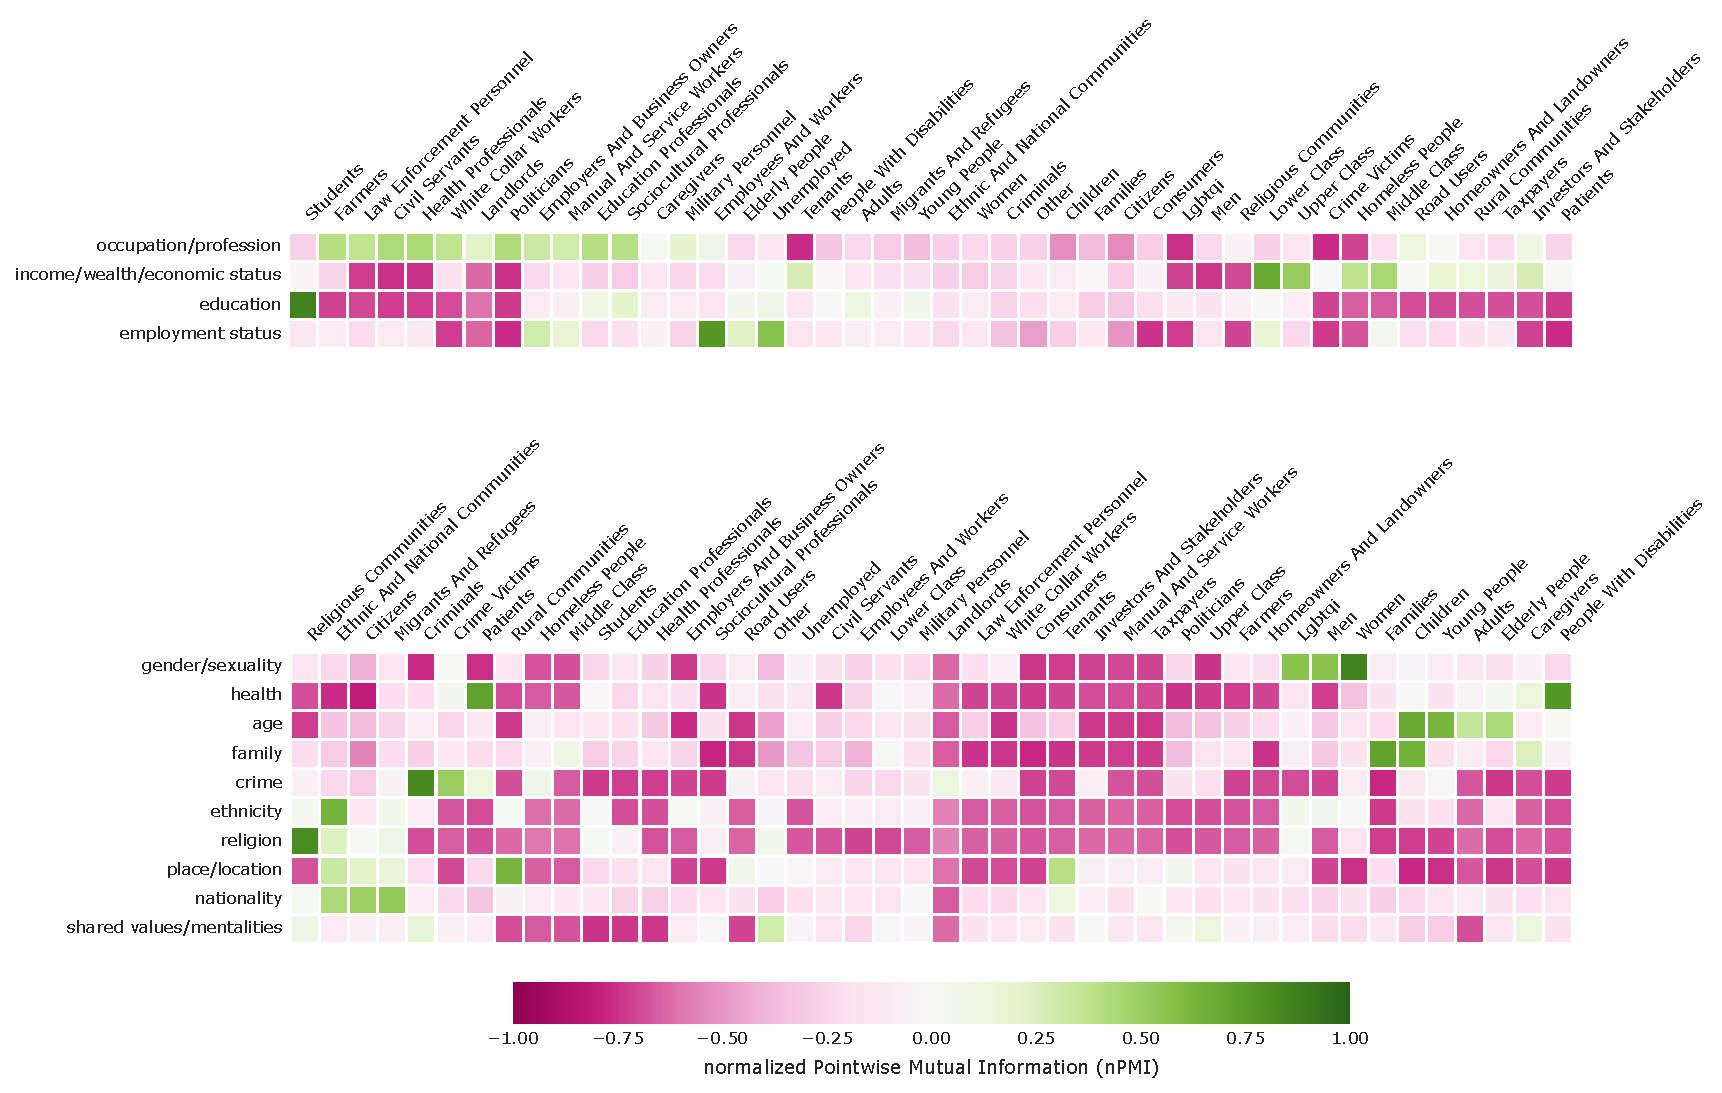
\includegraphics[keepaspectratio,width=\linewidth]{results/figures/figureC05.pdf}
  \caption{\label{figureC05}\protectPatterns of convergence between group mention classifications of our attribute-centered classifier and Horne et al.'s group category classifier. The figure reports normalized \emph{Pointwise Mutual Information} (nPMI) values that measure the strength of association of label classes on a scale ranging from -1 (systematic disassociation) through 0 (independence) to +1 (perfect co-occurrence).  y-axis labels indicate the attribute category in our scheme; x-axis labels the group categories in Horne et al.'s scheme. Plot panels separated by economic and non-economic attributes. \emph{Note:} heatmap columns sorted (for each attribute dimension) using hierarchical clustering to better reveal conceptual overlap.}
\end{figure}%

Figure~\ref{figureC05} presents the results of this analysis, reporting our attribute categories on the vertical axis and Horne et al.'s group categories along the horizontal axis (sorted to emphasize co-occurrence patterns).
Squares shaded green in Figure~\ref{figureC05} reveal expected convergence patterns, such as the strong co-occurrence tendency of our \emph{occupation/profession} attribute and Horne et al.'s occupation-related categories (e.g., \emph{Civil Servants}, \emph{Farmers}, \emph{Health Professionals}, etc.).
Squares shaded magenta, on the other hand, highlight the attribute categories that are systematically \emph{not} co-occurring with certain group categories in Horne et al.'s scheme.
For example, non-economic attributes like \emph{religion}, \emph{ethnicity}, and \emph{family} show consistent negative associations with occupation- and class-based group categories, because the group mentions sampled from our corpus are typically categorized as either occupation/class-based or non-economic but rarely both at the same time.
Taken together, these positive and negative association patterns reveal systematic similarities in how the two classification schemes partition the social group mention space: attributes that Horne et al.'s classifier treats as separate categories (e.g., occupation versus family status) show mutual exclusivity in their co-occurrence patterns.\footnote{A \(chi^2\)-test computed on the label category co-occurrence count matrix indicates a highly significant overall association between the two classification schemes (\(chi^2\) = 83,259.38, p \textless{} 0.001, Cramér's V = 0.633).}

However, Figure~\ref{figureC05} also shows that our attribute-centered approach groups some of Horne et al.'s more granular categories together (e.g., all occupation-related categories).
Other categories in Horne et al.'s scheme, like \emph{Ethnic And National Communities}, are represented as a mixture of \emph{ethnicity}, \emph{nationality}, \emph{religion}, and/or \emph{place/location} attributes in our scheme.
 
To shed more light on the convergence and divergences between our attribute classification and the group categorization scheme by Horne et al. (2025), we analyze the set of social group mentions labeled as featuring the \emph{occupation/profession} attribute and mentions labeled as featuring the \emph{gender/sexuality} attribute, respectively, in the subset of social group mentions in our machine-labeled corpus originally written in languages in which Horne et al.'s classifier has been evaluated.

This analysis of samples of social group mentions labeled as featuring \emph{occupation/profession}-related \emph{gender/sexuality}-related attributes, respectively, allows us to assess convergent validity by examining whether the sampled social group mentions are similarly categorized by Horne et al.'s group category classifier.
The dual classification creates overlapping annotations that reveal both areas of agreement (where both schemes identify similar patterns) and divergence (where our attribute-based approach captures distinctions not present in their categorical scheme).
This comparison helps assessing to what extent our attribute-centered framework aligns with established categorization but also adds analytical value.
Importantly, we examine these examples not to suggest that our classifiers have a higher accuracy but to illustrate how our attribute-centered approach seems to be better suited to accommodate attribute combinations because it puts all attribute categories on the same analytical level.

\subparagraph{\texorpdfstring{\emph{Occupation/profession}-related social group references}{Occupation/profession-related social group references}}\label{occupationprofession-related-social-group-references}

First, we focus on categories in Horne et al.'s classification scheme that capture references to specific occupational or professional groups.
In total, we identified 14 such categories in their scheme, ranging from \emph{Caregivers} to \emph{White Collar Workers}.\footnote{\emph{Caregivers}, \emph{Civil Servants}, \emph{Education Professionals}, \emph{Employees And Workers}, \emph{Employers And Business Owners}, \emph{Farmers}, \emph{Health Professionals}, \emph{Investors And Stakeholders}, \emph{Law Enforcement Personnel}, \emph{Manual And Service Workers}, \emph{Military Personnel}, \emph{Politicians}, \emph{Sociocultural Professionals}, \emph{White Collar Workers}}

Regarding convergence between their and our annotation scheme, we expect that our focus on occupation/profession-related attributes will lead to a high degree of overlap with mentions categorized into one or several of these categories by Horne et al.' classifiers.
This is confirmed by our analysis, which finds that the share of mentions labeled as expressing an \emph{occupation/profession} attribute by our classifier that are classified into an occupation group category by Horne et al.'s classifier is 84\% -- a high degree of correspondence.

\begin{figure}[!th]

  \centering
  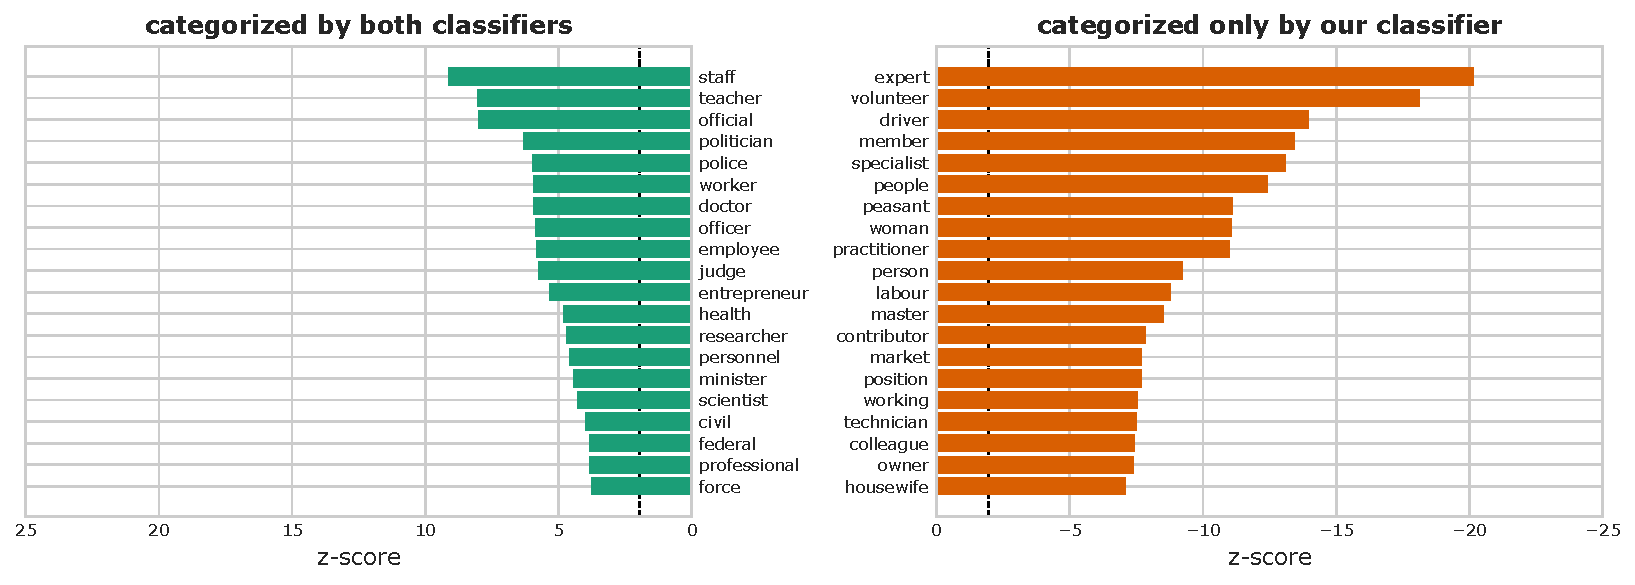
\includegraphics[keepaspectratio,width=\linewidth]{results/figures/figureC06.pdf}
  \caption{\label{figureC06}\protectMost distinctive words for mentions labeled as featuring occupation/profession as an attribute by our classifier depending on whether Horne et al.'s classifier has classified them into (at least) one of their occupation/profession-related categories (left) or not (right). Values plotted are $z$-scores from ``fighting words'' analysis of occupation/profession mentions. Values above ±1.96 (vertical dashed line) can be considered significantly distinctive.}

\end{figure}%

\begin{table}[!th]
\centering
\caption{Examples of social group mentions labeled as featuring occupation/profession as an attribute by our classifier that were not assigned to any of Horne et al.'s occupation-related group categories by their classifier. Values computed by summing ``fighting words'' scores as weights of mentions' tokens, normalized by number of tokens.}
\label{tableC11}
\begin{tabular}{p{3in} l l}
\toprule
Mention & $z$-score & Horne et al. classification \\
\midrule
International experts & -20.157 &  \\
The volunteers & -18.135 & Other \\
the people smuggler & -12.406 & Criminals \\
-competent people & -12.406 &  \\
environmental experts across Britain & -11.563 & Other \\
experts of interest organisations & -11.526 &  \\
low-skilled women & -11.089 & Women \\
returning volunteers & -9.098 & Other \\
unskilled tax experts who believe to know & -8.603 &  \\
a car and motorcycle driver & -7.419 & Road Users \\
a committee of specialists & -6.954 &  \\
drivers who continue their training in economical and environmentally friendly driving & -6.177 &  \\
human rights representatives in all German embassies & -5.366 & Other \\
legal practitioners & -5.351 &  \\
rail users & -4.652 & Road Users \\
Anyone who collects data and works with it & -4.476 &  \\
concrete and direct owners of what has been & -3.485 & Homeowners And Landowners \\
the respective stakeholder representatives & -3.192 & Other \\
union stakeholders & -2.521 & Other \\
those most directly involved in some of the economic organisations we already have & -2.324 &  \\
\bottomrule
\end{tabular}
\end{table}
%

However, we also expect that due to being more encompassing and abstract than some of Horne et al.'s categories, such as \emph{Civil servants}, \emph{Farmers}, \emph{Health professionals}, etc., our \emph{occupation/profession} attribute will capture a broader set of mentions.
We again assess this question through a ``fighting words'' analysis to identify \(n\)-gram patterns that distinguish the 18\% of social group mentions labeled as featuring the attribute of \emph{occupation/profession} by our classifier that are not classified into any of Horne et al.'s occupation-related categories.
Figure~\ref{figureC06} and Table~\ref{tableC11} show that our \emph{occupation/profession} classifications capture occupational and professional groups not covered by Horne et al.'s schemes, including broad categories like ``experts'' and ``practitioners'' as well as specific categories like ``drivers''.

\subparagraph{\texorpdfstring{\emph{Gender/sexuality}-related social group references}{Gender/sexuality-related social group references}}\label{gendersexuality-related-social-group-references}

Turning to mentions that feature attributes related to gender and/or sexuality, we perform a similar cross-validation exercise by comparing their overlap with classifications into Horne et al.'s group categories \emph{LGBTQI}, \emph{Men}, and \emph{Women}.
Again, we find a high overlap between classifications.
91.9\% of mentions labeled as expressing a \emph{gender/sexuality} attribute by our classifier are classified into (at least) one of Horne et al.'s \emph{LGBTQI}, \emph{Men}, or \emph{Women} group categories by their classifier.

\begin{figure}[!th]

  \centering
  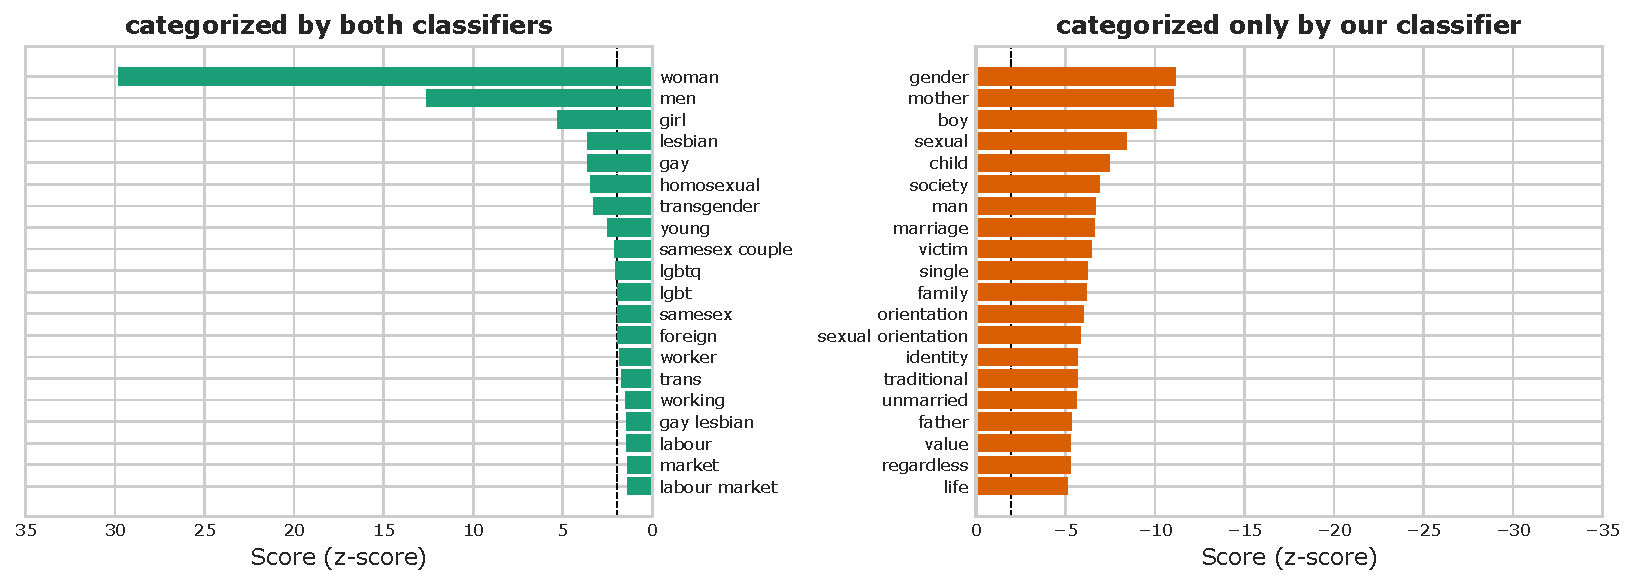
\includegraphics[keepaspectratio]{results/figures/figureC07.pdf}
  \caption{\label{figureC07}\protectTop 20 most distinctive words for gender/sexuality mentions classified by Horne et al. (right) vs. not classified (left).}

\end{figure}%

\begin{table}[!th]
\centering
\caption{Examples of social group mentions labeled as featuring gender/sexuality as an attribute by our classifier that were not assigned to any of Horne et al.'s Men, Women, or LGBTQI categories by their classifier. Values computed by summing ``fighting words'' scores as weights of mentions' tokens, normalized by number of tokens.}
\label{tableC12}
\begin{tabular}{p{3in} l l}
\toprule
Mention & $z$-score & Horne et al. classification \\
\midrule
all genders & -11.141 &  \\
specialized agents on gender issues & -11.141 & Law Enforcement Personnel \\
Familial mothers & -11.036 & Families \\
mothers of 1 or 2 children & -9.258 & Families \\
mothers who have raised at least three children or raised a disabled child & -9.258 & Families \\
a mother and father who & -8.193 & Families \\
a mother who are married & -8.027 & Families \\
the family of father, mother and children & -7.512 & Families \\
people of each gender & -6.715 & Other \\
those who are practically single & -6.250 & Families \\
A society built on solidarity and where we stand up for gender equality and justice & -5.800 & Other \\
everyone, regardless of economics, gender and social status & -5.662 & Other \\
widowed mothers & -5.641 & Families \\
people of all races, religions, sexual orientations, and gender identities & -5.081 &  \\
two cohabitants (married or not & -5.018 & Families \\
People who are not safe in their country on individual grounds (such as sexual orientation, political beliefs or religion & -4.469 & Other \\
mothers and fathers who want to reduce their daily working hours in order to have time for their children & -4.365 & Families \\
couples, whether in marriage & -4.106 & Families \\
well-educated sisters, who have already experienced equality in everyday life & -3.432 & Families \\
fathers who have given up on work after the birth of their children & -3.037 & Families \\
\bottomrule
\end{tabular}
\end{table}
%

However, looking at the remaining mentions that we label as \emph{gender/sexuality}-related but not Horne et al.'s classifier, we again find interesting patterns.
Most common are mentions including the familial role ``mother'' (see Figure~\ref{figureC07}), some of which combine this attribute with qualifiers (see Table~\ref{tableC12}).

\section{Additional results}\label{additional-results}

\subsection{Attribute category focus by party family}\label{attribute-category-focus-by-party-family}

\begin{figure}[!th]

  \centering
  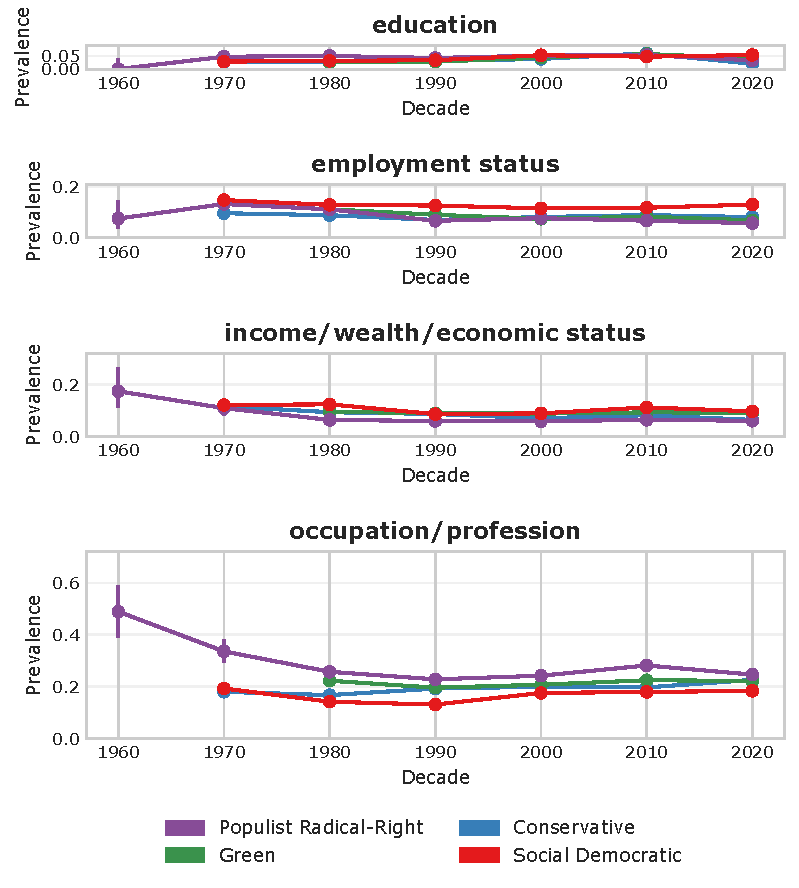
\includegraphics[keepaspectratio]{results/figures/figureD01.pdf}
  \caption{\label{figureD01}\protectTemporal trends in the prevalence of economic attributes in social group mentions by PRR and Green parties across decades. Each panel shows one economic attribute category, with error bars representing 95\% confidence intervals. Lines show the share of mentions containing each attribute over time.}

\end{figure}%

Figure~\ref{figureD01} and Figure~\ref{figureD02} show that the differences between PRR and Green parties' group attribute focus shown in Figure~\ref{figure05} exhibit interesting temporal patterns.
Figure~\ref{figureD01} shows that while their relative emphasis differences are overall very stable across decades, PRR parties' overall stronger focus on the \emph{occupation/profession} attribute is more pronounced in the 1970s than in later decades.
Regarding non-economic attribute prevalence, Figure~\ref{figureD02} shows that Green parties' \emph{age} focus stands out especially in the 2000s and 2010s, whereas their \emph{gender/sexuality} focus has been relatively more pronounced before the 2000s.
PRR parties' group focus, in turn, shows a sharp increase in the prevalence of \emph{family} from 2010s to 2020s.

\begin{figure}[!th]
  \centering
  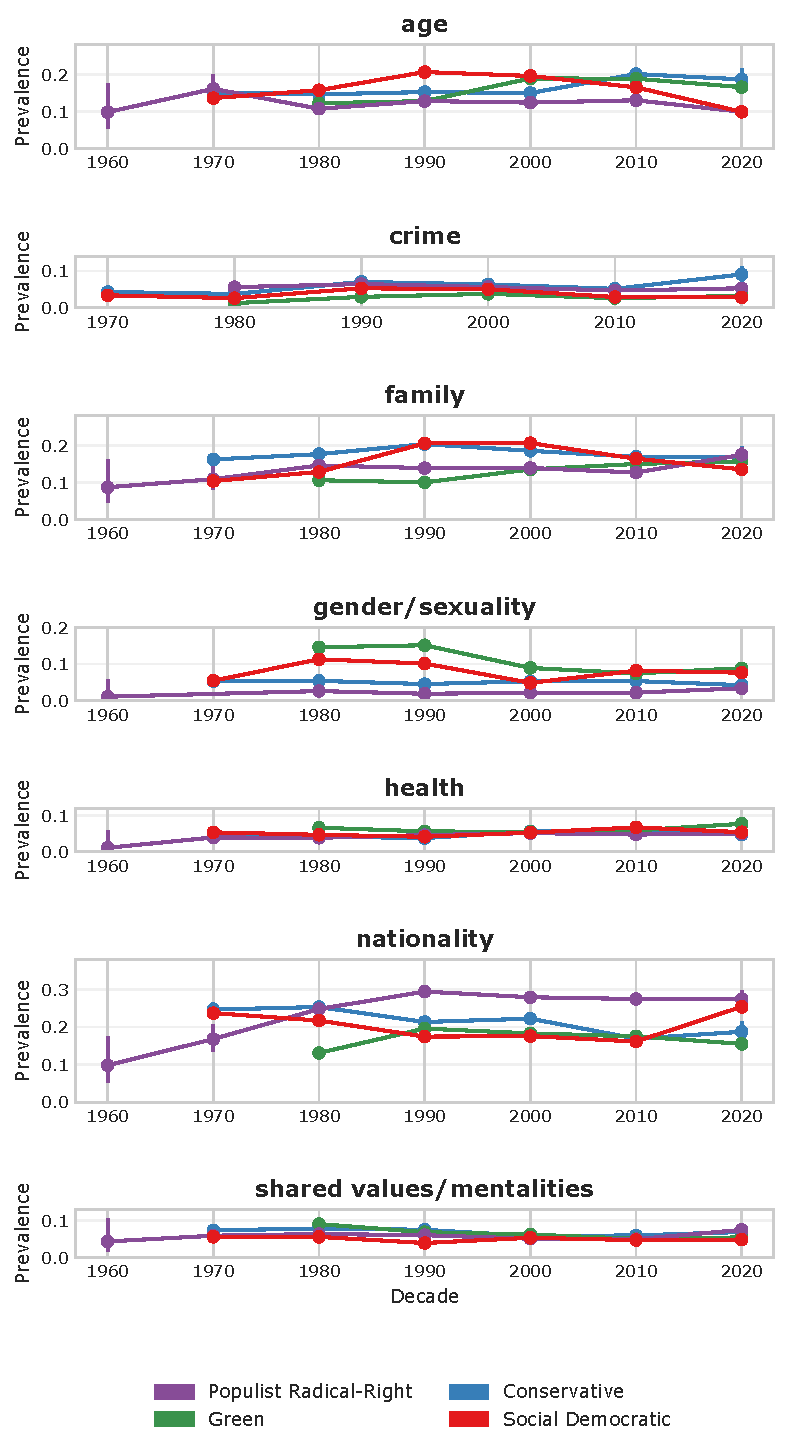
\includegraphics[keepaspectratio]{results/figures/figureD02.pdf}
  \caption{\label{figureD02}\protectTemporal trends in the prevalence of economic attributes in social group mentions by PRR and Green parties across decades. Each panel shows one economic attribute category, with error bars representing 95\% confidence intervals. Lines show the share of mentions containing each attribute over time.}
\end{figure}%

\subsubsection{Representativeness of our mainstream party selection}\label{sec-apx_case_selection_robustness}

Our case selection strategy aims to cover Green and PRR parties as comprehensively as possible while covering Social Democratic and Conservative parties in four selected countries.
Below, we replicate our analysis of the prevalence of attribute dimensions and categories to assess the representativeness of the cases in the four countries in which we also cover Social Democratic and Conservative parties.

This analysis relies on the \emph{Manifesto Corpus Translations} corpus (Ivanusch and Regel 2024) that records full-text translations for a subset of the manifestos in the Manifesto Corpus.
This data allows us to apply our group mention detection and attribute classifiers also to (quasi-)sentences in cases we have not originally covered in our case selection.

The caveat of this corpus -- and the reason we have not based our raw data collection solely on it -- is that the translations are only available for manifestos for which the Manifesto Corpus records quasi-sentence level annotations.
This is largely only the case for manifestos from elections in the 1990s and later decades -- a much shorter period than we are able to cover through complementary data collection.

As a consequence, only 72 of the 110 mainstream party manifestos covered in our corpus are also covered in the \emph{Manifesto Corpus Translations} corpus (37 from Social Democratic and 35 from Conservative and Christ-Democratic parties).
Yet, the upside of using the \emph{Manifesto Corpus Translations} corpus is that we can cover an additional 492 manifestos (291 Conservative/Christ-Democratic and 201 Social Democratic) in the countries in our case selection.

\afterpage{
  \clearpage
  \thispagestyle{empty}
  \begin{figure}[p]
    \centering
    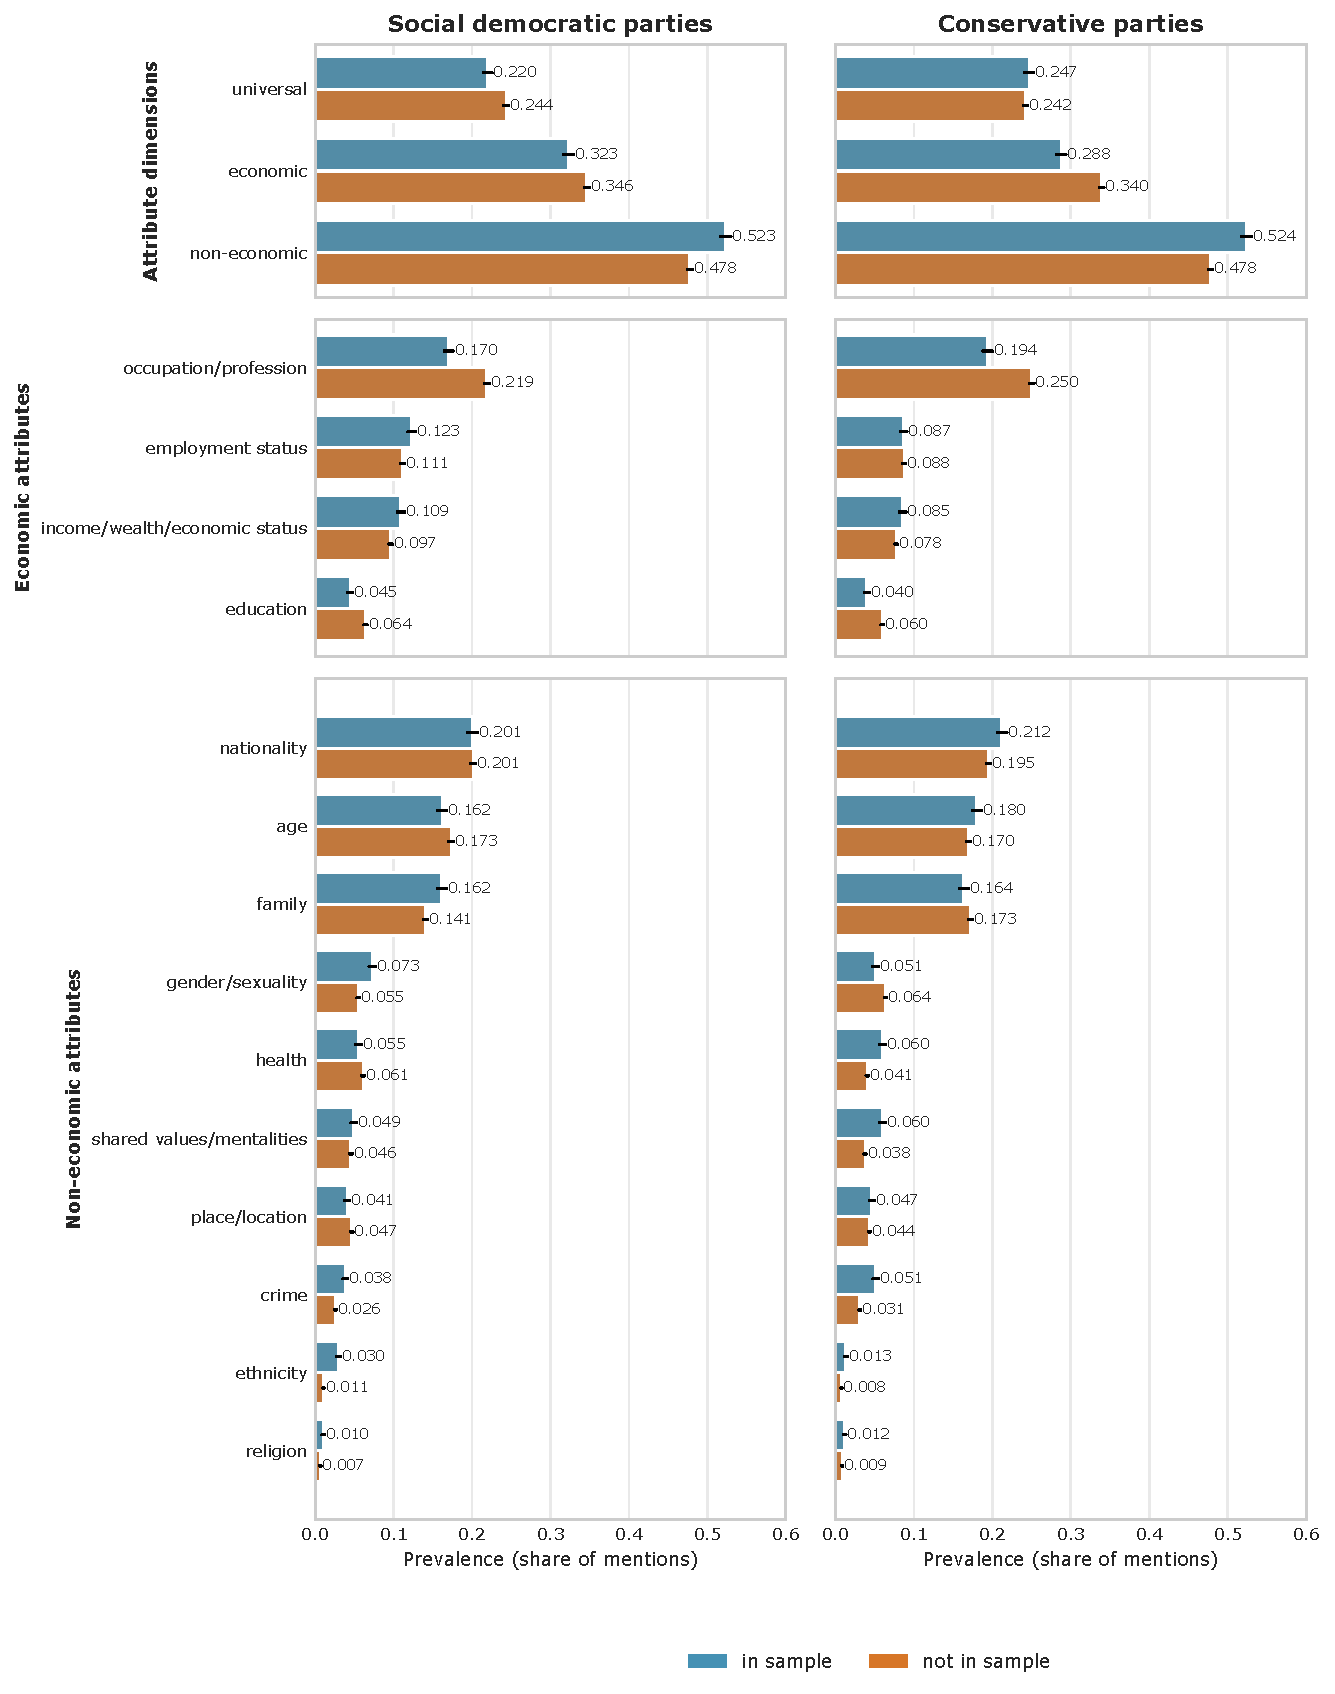
\includegraphics[keepaspectratio,width=\linewidth]{results/figures/figureD03.pdf}
    \caption{\label{figureD03}\protectPrevalence of attribute dimensions in all mentions and economic and non-economic attributes in non-universal social group mentions in parties' election manifestos by party family. Bars show share of mentions containing each attribute, with 95\% confidence intervals. \emph{Note:} Top panel shows prevalence in all mentions, while middle and bottom panels show prevalence in mentions containing at least one attribute.}
  \end{figure}%
  \clearpage
}

Figure~\ref{figureD03} shows that for most attribute dimensions and categories, the prevalence estimates for parties included and excluded in our case selection are very similar.
However, we observe the following (slight) deviations (compare also to Figure~\ref{figure05}):

\begin{itemize}
\tightlist
\item
  economic dimension: We underestimate Conservative parties' focus on economic attributes. Adjusting for this makes their emphasis of economic attributes about as high as that of Social Democratic and PRR parties
\item
  non-economic dimension: We slightly overestimate Social Democratic and Conservative parties' focus on non-economic attributes. Adjusting for this makes their emphasis of non-economic attributes about as high as that of Green and PRR parties.
\item
  \emph{occupation/profession}-related attributes: We slightly underestimate Social Democratic and Conservative parties' focus on occupation/profession. In pure comparison to Green and PRR parties, this makes these parties (but especially PRR parties) seem slightly more outstanding in this regard than they are in this sample with broader coverage
\end{itemize}

It is worth noting, however, that the differences in prevalence can also be due to differences in the temporal coverage of our case selection and that allowed by relying on the Manifesto Corpus Translation corpus.

\subsection{Conditional probabilities of attribute category co-occurrences}\label{conditional-probabilities-of-attribute-category-co-occurrences}

An alternative approach to quantatively describing attribute co-occurrence patterns is to compute the conditional probabilities of co-occurrence.
We can compute \(\Pr(\text{attribute B} \mid \text{attribute A})\) for attribut category pairs and compare these values.
Conditional probabilities have the advantage that they are very interpretable, allowing statements like ``When a party uses \emph{economic status} to describe a group, the probability that it also uses \emph{gender/sexuality} in the group mention is 0.12.''
Conditional probabilities thus directly answers substantive questions about co-occurrence patterns.
Further, they do not suffer from base rate sensitivity issues.

The downside is that the measure is asymmetric, requiring careful interpretation.
Further, it does not account for statistical significance of observed differences.
We therefore use it solely for \emph{descriptive} comparison of party families' attribute combination strategies.

\afterpage{
  \clearpage
  \thispagestyle{empty}
  \begin{figure}[p]
    \centering
    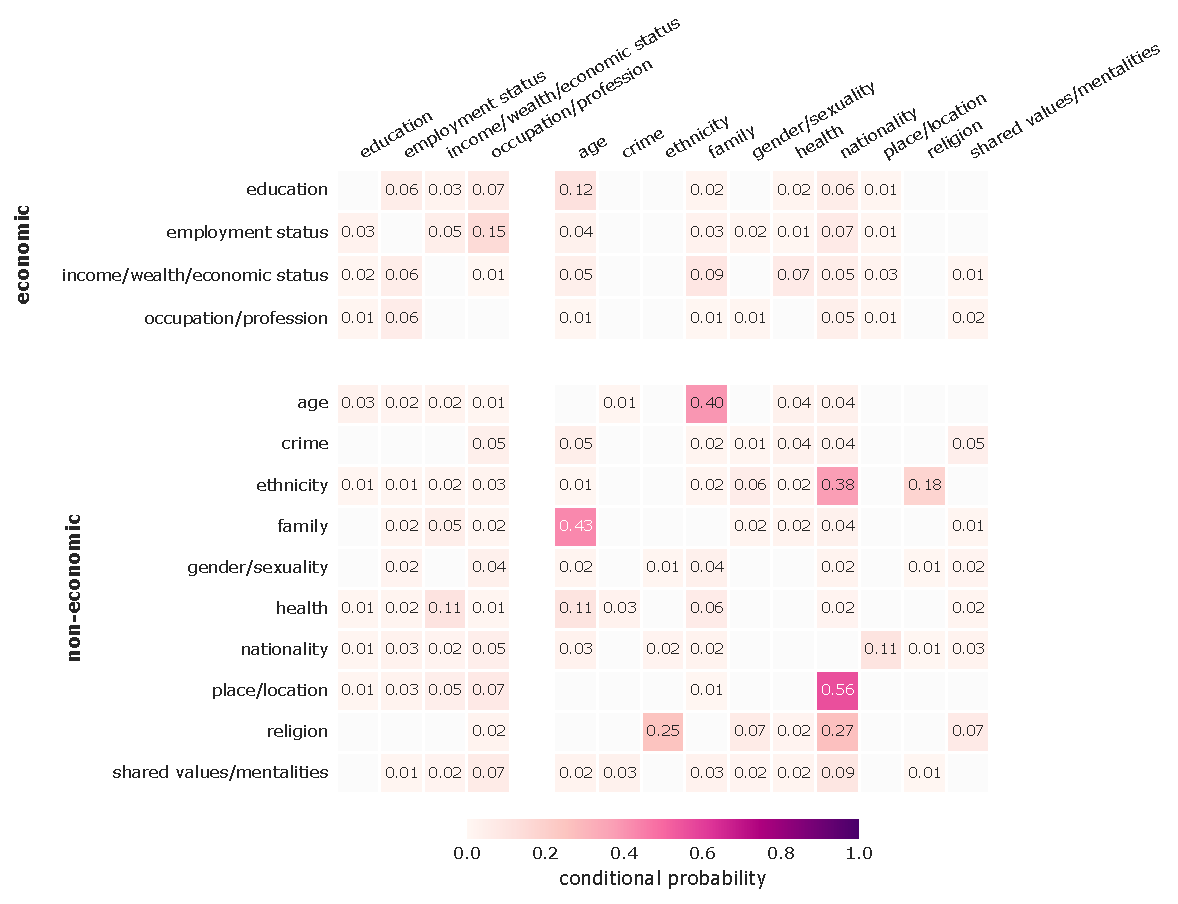
\includegraphics[keepaspectratio,width=\linewidth]{results/figures/figureD04.pdf}
    \caption{\label{figureD04}\protectConditional probabilities of attribute co-occurrence in social group mentions. Heatmap cells show P(B|A), the probability of mentioning attribute B given that attribute A is mentioned. Rows indicate "attribute A" (the conditioning attribute) and columns indicate "attribute B" (the outcome attribute). \emph{Note:} Values below 0.01 are not displayed.}
  \end{figure}%
  \clearpage
}


\afterpage{%
  \clearpage%
  \thispagestyle{empty}%
  \begin{landscape}%
  \begin{table}[!th]
\centering
\label{tableD01}
\begin{tabular}{p{3cm} p{3cm} r p{2.5cm} p{2.5cm} p{2.5cm} p{2.5cm} p{2.5cm}}
\toprule
attribute a & attribute b & Pr(b | a) & example 1 & example 2 & example 3 & example 4 & example 5 \\
\midrule
place/location & nationality & 0.562 & the population of Africa, including all Arab countries & people in the global South & Foreigners living in Germany & Foreigners residing in Flanders & Nordic citizens who have had a permanent residence in the country for 3 years \\
family & age & 0.429 & children & children & children & children & children \\
religion & nationality & 0.269 & Muslims in France & persecuted minorities in authoritarian states & the second largest religious group in Germany & Islamic faith communities in Germany & most of us \\
religion & ethnicity & 0.255 & a multi-ethnic society & its diverse society & Black and Latino communities & ethnic and cultural minorities & those who attack or derogate any race or creed \\
health & income/wealth/economic status & 0.113 & , who cannot afford the necessary "extras" in medical care from their own pockets & those affected & vulnerable residents & persons with reduced mobility & the affected \\
health & age & 0.107 & healthy and confident young people who have quality medical care & preschool children with special needs & young people with special support needs & the elderly and disabled & elderly people in need of care \\
\bottomrule
\end{tabular}
\end{table}
%
  \end{landscape}%
  %\clearpage%
}%


\end{document}
